\documentclass[12pt,twoside]{article}

% La extensión total de la memoria deberá ser de un máximo de 50 páginas (excluidos resumen, índice y posibles anexos).

% Según las recomendaciones de estilo, el formato de la memoria se ajustará a lo siguiente:
% ? Formato del papel: DIN A4.
% ? Impresión a dos caras.
% ? Márgenes: superior e inferior, 2.5 cm. Márgenes laterales: páginas impares, izquierdo 4 cm y derecho 2 cm; páginas % pares, izquierdo 2 cm y derecho 4 cm.
% ? Tipo de letra: Times New Roman de 12 puntos.
% ? Interlineado: 1.5 líneas.
% ? Alineación: justificación completa.
% ? Sangrado de párrafo: 0.5 cm la primera línea de cada párrafo. No se
%pondrá espacio entre párrafos.
% ? Las páginas deberán ir numeradas en números arábigos.

% Teniendo en cuenta las indicaciones previas, definimos el estilo en LaTeX:

% Indicaciones para el idioma:
\usepackage[T1]{fontenc}
\usepackage{hyperref}
\hypersetup{     
    pdftitle={El modelo de Hubbard en materia condensada},
    colorlinks=true,
    linkcolor=black,
    citecolor=black,
    urlcolor=black,
    }
\urlstyle{same}
\usepackage[utf8]{inputenc}
\usepackage[spanish]{babel}
\usepackage[backend=biber]{biblatex}
\usepackage[export]{adjustbox}
\newcommand\labelAndRemember[2]
  {\expandafter\gdef\csname labeled:#1\endcsname{#2}%
   \label{#1}#2}
\newcommand\recallLabel[1]
   {\csname labeled:#1\endcsname\tag{\ref{#1}}}
\addbibresource{TFG.bib}
% Adaptación de itemize y enumerate a los usos tipograficos españoles:
\let\layoutspanish\relax
\addto\captionsspanish{\def\tablename{Tabla}} % para que escriba "Tabla" en lugar de "Cuadro"
\unaccentedoperators  % para que no acentúe los operadores

% Área de impresión de una página:
\usepackage[a4paper]{geometry}
  \geometry{hmargin={2.5cm,2.5cm},height=22cm}

% Formato de algunas distancias:
\renewcommand{\baselinestretch}{1.2}    % separación entre líneas de un mismo párrafo
\setlength{\partopsep}{0pt}
\setlength{\itemsep}{0pt}
\setlength{\topsep}{0pt}
\setlength{\parsep}{0pt}
\setlength{\parskip}{0.25\baselineskip}   % separación entre párrafos

\renewcommand{\textfraction}{0.1}   % mínima fracción de la página para el texto
\renewcommand{\topfraction}{1}      % máxima fracción de la página para objetos flotantes en la parte superior
\renewcommand{\bottomfraction}{1}
\renewcommand{\floatpagefraction}{1}

\setcounter{totalnumber}{5}
\setcounter{topnumber}{3}
\setcounter{bottomnumber}{2}

% Adaptación de las "caption" de los entorns "figure" y "table":
\usepackage{caption}
\addtolength{\textwidth}{-2\parindent}
\captionsetup{margin=\leftmargini,%
  width=\textwidth,%
  labelfont={up,bf},%
  font={small,sl},%
  %indention={\captionindent
}

% Indentación del primer párrafo de una sección:
\usepackage{indentfirst}

% Definición del color grisclaro en la salida PDF:
\usepackage[pdftex]{color}

% Gráficos:
\usepackage{graphicx}
% Paquetes recomendados para la inclusión de fórmulas matemáticas:
\usepackage{amsmath}
\allowdisplaybreaks  % para que pueda partir fórmulas que ocupan más de una línea, necesita el paquete anterior
\usepackage{amssymb} % para cargar algunos símbolos como \blacksquare y \square
\usepackage{amsfonts} % para cargar algunas fuentes en estilo matemático
\usepackage{enumerate}
% Teoremas (se pueden definir todos los que se necesiten):

%\newtheorem{theorem}{Teorema}[section]
%\newtheorem{proposition}[theorem]{Proposición}
%\newtheorem{definition}[theorem]{Definición}
%\newtheorem{lemma}[theorem]{Lema}
%\newtheorem{corollary}[theorem]{Corolario}
%\newtheorem{example}[theorem]{Ejemplo}
%\newtheorem{app}[theorem]{Aplicación}
%\newtheorem{remark}[theorem]{Observación}
%\newtheorem{agrad}[theorem]{Agradecimiento}
%\newtheorem{algo}[theorem]{Algoritmo}
%\newtheorem{axiom}[theorem]{Axioma}
%\newtheorem{case}[theorem]{Caso}
%\newtheorem{conclu}[theorem]{Conclusión}
%\newtheorem{conjectura}[theorem]{Conjetura}
%\newtheorem{notac}[theorem]{Notación}
%\newtheorem{soluc}[theorem]{Solución}
%\newtheorem{summary}[theorem]{Sumario}


%\newtheorem{proof}[theorem]{Demostración.}
%\renewenvironment{proof}{\emph{Demostración.}} {\quad \hfill $\blacksquare$ \newline} % para que aparezca un cuadrado negro al acabar la demostración


% Definición de cabeceras y pies de página:

\usepackage{fancyhdr}                     % para definir distintos tipos de cabeceras y pies de página

\newcommand{\RunningAuthor}{Luis Lucas García}
\newcommand{\Author}[1]{\renewcommand{\RunningAuthor}{#1}}
\renewcommand{\leftmark}{\RunningAuthor}

\newcommand{\RunningTitle}{Trabajo de fin de grado}
\newcommand{\Title}[1]{\renewcommand{\RunningTitle}{#1}}
\renewcommand{\rightmark}{\RunningTitle}

\pagestyle{fancy}
\fancyhf{}
\fancyhead[LO]{\small \slshape \leftmark}    % lo que aparece en la parte izquierda de la páginas impares
\fancyhead[RE]{\small \slshape \rightmark}   % lo que aparece en la parte derecha de las páginas pares
\fancyhead[RO,LE]{\small \slshape \thepage}  % el número de página aparece en la parte exterior de la cabecera

\renewcommand{\headrulewidth}{0.6pt}         % grueso de la línea horizontal por debajo de la cabecera de la página
\renewcommand{\footrulewidth}{0pt}           % grueso de la línea horizontal por encima del pie de página
                                             % en este caso está vacío
\setlength{\headheight}{1.5\headheight}      % aumenta la altura de la cabecera en una parte y media

\fancypagestyle{plain}{%                     % redefinición del estilo de página 'plain'
  \fancyhf{}                                 % limpia todas las cabeceras y pies de página
  \setlength{\headwidth}{\textwidth}
  \fancyfoot[C]{\small \slshape \thepage}    % excepto el centro del pie de página
  \renewcommand{\headrulewidth}{0pt}
  \renewcommand{\footrulewidth}{0pt}
  }

% Instrucciones que se usan frecuentemente
\newcommand{\abs}[1]{\ensuremath{|#1|}}

% Datos del trabajo y autor:
\title{El modelo de Hubbard en materia condensada}
\author{Luis Lucas García\\*[1em]
\begin{minipage}{0.75\textwidth}
\footnotesize \itshape
\begin{center}
Universidad de Alicante \\
4º de Grado en Física
\end{center}
\end{minipage}
}
\date{Junio 2025}

% Para incluir paginas de otro pdf (por ejemplo, la de la portada):
\usepackage{pdfpages}
\graphicspath{{../Imágenes}}


\begin{document}

% Para introducir la portada en castellano, se guardar anexo-1-portada-memoria-tfg-matematicas.pdf en el mismo directorio:
\includepdf[pages=1]{anexo-1-portada-memoria-tfg-fisica.pdf}


% Después de la portada, se introducirá un resumen del Trabajo Fin de Grado (máximo 500 palabras) en una de las lenguas oficiales y en inglés, junto con las palabras clave (de 3 a 5).

\section*{Resumen}

\emph{En este TFG se propone estudiar un modelo que permite describir simplificadamente las interacciones electrónicas dentro de un sólido. Este modelo es el modelo de Hubbard. Está basado en una descripción del material utilizando la aproximación de ligadura fuerte que se estudia en la asignatura de física del estado sólido del 4º curso. Para escribir el Hamiltoniano que describe este modelo necesitaremos también familiarizarnos con el formalismo de segunda cuantización que se estudia también en la optativa de 4º curso de física cuántica avanzada. La primera parte del trabajo consistirá entonces en estudiar los fundamentos teóricos del problema y escribir el Hamiltoniano correspondiente \cite{alma9947259002101}. El Hamiltoniano parece sencillo, sin embargo, contiene casi todos los fenómenos interesantes que se observan en los materiales: orden magnético, transiciones de fase, superconductividad etc. De allí el interés de comprenderlo y aprender a resolverlo. La complejidad del problema hace que haya pocos resultados rigurosos sobre el mismo, y en general se apela a diferentes tipos de aproximaciones o soluciones numéricas en redes no demasiado grandes. Nuestro objetivo será este último, desarrollando un algoritmo de diagonalización exacta, basado en el método de Lanczos de tridiagonalización de matrices para obtener el estado fundamental del modelo en redes cristalinas finitas en 1 dimensión con condiciones de contorno abiertas. Una vez obtenido el estado fundamental el interés será obtener sus propiedades espectrales. Esto se puede realizar aplicando el formalismo de funciones de Green para el calculo de funciones de correlación \cite{fetter2003quantum}, que permite obtener propiedades como la densidad de estados en función de la energía \cite{RevModPhys.66.763}.}

\newpage

\section*{Abstract}

\emph{In this thesis we propose the study of a model that allows a simple description of the electronic interactions within a solid. This is Hubbard's model. It's based in a description of the material using the tight-binding aproximation, that's studied in the 4th course of the physics degree, in the solid state physics subject. To write the hamiltonian that describes this model we will need to familiarize ourselves with the second quantization formalism which is studied in the advanced quantum physics subject. The first part of this thesis will consist on the study of the theoretical foundations of the problem and writing the corresponding hamiltonian \cite{alma9947259002101}. The hamiltonian may look simple, however, it contains almost all of the interesting phenomena observed in the materials: magnetic order, phase transitions, superconductivity, etc. From that, comes the interest in understanding it and learning how to solve it. The complexity of the problem leads to few rigorous results existing on the model, and, in general, we appeal to different kinds of approximations or numerical solutions in not-so-big lattices. Our objective will be this numerical solutions, we will develop an exact diagonalization algorithm, based on the Lanczos' tridiagonalization of mattrices to obtain the ground state of the model in finite 1-dimensional lattices with open boundary conditions. Once the ground state is obtained it is of interest obtaining the spectral properties. This can be done applying the Green's functions formalism for the calculation of correlation functions \cite{fetter2003quantum}, that allows us to obtain properties such as the density of states as a function of the energy \cite{RevModPhys.66.763}.}

% A continuación, se incluirá el índice del trabajo y, seguidamente, se desarrollará la memoria.
\newpage

\section*{Agradecimientos}

Quiero agradecer a Conchi, mi tutora en tercero de la ESO y profesora desde tercero hasta primero de bachillerato de física y química. Gracias por encender la llama de la física en mí, y hacerme elegir un camino muy distinto al que yo pensaba que era para mí. Ahora me he dado cuenta de que esto sí es lo mío, todos esos profesores que hacen de guía a sus alumnos, nunca dejéis de orientar con vuestros consejos, ánimos y conocimiento a los demás.

A mi pareja, Miguel, por aguantarme día sí y día también y apoyarme en todo lo que hago. Y también por quedarse conmigo el viernes hasta las tres de la mañana mientras acababa de escribir este documento. Eres la mejor compañía que podría haber tenido estos tres últimos años.

A mi familia, mi madre Luisa y Antonio por ayudarme, viviendo fuera de casa y apoyándome cuando estaba en Torrevieja escribiendo estas últimas páginas. También a mi padre, Jose, por sus visitas esporádicas a San Vicente, que me ayudaban a salir de la rutina.

A mis amigos de Torrevieja por las noches de fiesta en el Alchemist, pero también por las partidas de rol interminables o las tardes de juegos de carta y también a mis amigos de San Vicente, por esas noches interminables en el salón de mi piso.

Finalmente, agradecer a la Asociación para la Cultura Furry Española (ACFE), por haber hecho de este 2025 el año más especial de todos, y darme la oportunidad de organizar las actividades de Ibercon. A ellos sólo les digo: mirad lo que hemos conseguido.
\begin{figure}[h!]
  \begin{center}
    \includegraphics[max width=\linewidth]{Ibercon.png}
    \caption{Copyright cedido por ACFE y permiso por el propio fotógrafo.}
  \end{center}
\end{figure}

\newpage

\tableofcontents

\newpage

\section{Introducción}

En este trabajo vamos a estudiar el modelo de Hubbard. Este modelo permite describir, a partir de la aproximación de ligadura fuerte, ciertas formas de interacción entre electrones en sólidos. Para ello, nos vamos a centrar a lo largo de este trabajo en el caso unidimensional. De este modo, este trabajo va a estar fuertemente centrado en los aspectos teóricos y numéricos.

Este modelo, aunque sencillo, presenta varios fenómenos interesantes de la materia condensada: transiciones de fase, superconductividad, etc. Nos permitirá aplicar los conocimientos de la asignatura de estado sólido en un modelo algo más complejo.

Además, el modelo de Hubbard resulta de gran interés para la superconductividad de altas temperaturas. En tiempos más recientes, se ha utilizado el modelo para describir el comportamiento de átomos ultrafríos atrapados en redes ópticas. También se han realizado experimentos sobre estos átomos, con la esperanza de poder generar un diagrama de fases.

El término de Hubbard, $U$, también es utilizado en simulaciones DFT basadas en primeros principios y la inclusión de dicho término en las simulaciones es importante, puesto que ayuda a determinar la localización de electrones e impide que las simulaciones predigan conductividad en materiales que son aislantes.

Aunque en este trabajo nos vamos a centrar en el modelo de fermiones con interacción a primeros vecinos, existe también un modelo de bosones (modelo de Bose-Hubbard) y un modelo ampliado, que considera interacciones a cualquier posición de la red. Más adelante veremos a que nos referimos con esto.

Nuestro objetivo a lo largo de este trabajo será la obtención del estado fundamental y sus autoestados de forma numérica para una pequeña red unidimensional. Más adelante podremos obtener un espectro de excitaciones para el problema, así como la densidad de estados, gracias al formalismo de las funciones de Green, que también aplicaremos numéricamente gracias al algoritmo de Lanczos.

Aunque no tardaremos en descubrir, que la complejidad numérica del modelo crece muy rápidamente, en memoria y en tiempo de computación, por lo que nos restringiremos a cadenas pequeñas, de como mucho 10 átomos. En este trabajo se describirá una cadena de átomos con un único orbital, pero podrían describirse modelos más complejos.
\newpage
\section{Fundamentos teóricos}

Aunque a primera vista simple, el hamiltoniano de Hubbard contiene varios fenómenos físicos de gran importancia en la física de materia condensada. Podemos encontrar que el hamiltoniano de Hubbard en una red cualquiera tiene la siguiente forma \cite{MielkeHubbard}:
\begin{equation}
  \labelAndRemember{eq:hubbardHam}{H = \sum_{x, y, \sigma}t_{xy}c^{\dagger}_{x,\sigma}c_{y,\sigma} + \sum_x U_x c^{\dagger}_{x\uparrow}c^{\dagger}_{x\downarrow}c_{x\downarrow}c_{x\uparrow}}
\end{equation}

Sin embargo, este hamiltoniano presenta muchos conceptos de los que no tenemos porqué conocer todos. Para empezar, este hamiltoniano considera términos de hopping (el término denominado $t_{xy}$) que pueden ocupar todos los puntos de la red. Muchas veces consideramos por simplicidad un término de hopping a primeros vecinos, que viene definido por:
\begin{equation}
  t_{xy} = \left\{\begin{array}{cc}
    t, & |x - y| = 1 \\
    0, & \text{en otro caso}
  \end{array}\right.
  \label{eq:hoppinFN}
\end{equation}

De aquí entenderemos en este punto poco o nada. Con una base de mecánica cuántica sabemos lo que es un hamiltoniano y quizás sepamos algo sobre los operadores que conforman el de la ecuación (\ref{eq:hubbardHam}) puesto que nos recuerdan a los operadores de creación y destrucción que aparecían a la hora de resolver el oscilador armónico cuántico. En efecto, el operador $c_{x,\sigma}$ es el operador de destrucción actuando sobre una partícula en la posición $x$ con spin $\sigma$.

Pero, ¿cómo hemos llegado a este operador? ¿Qué es lo que podemos extraer del mismo? ¿De dónde sale el hamiltoniano de más arriba? Para entender todo esto necesitamos entender el formalismo de segunda cuantización y de las funciones de Green, así como algunos conceptos de física de estado sólido. Pero para entender todo esto necesitamos una nueva visión de los operadores en la mecánica cuántica, donde el tiempo está ligado a estos mismos y no a la función de onda.
\subsection{Representación de Heisenberg}

Hasta ahora, en los cursos de mecánica cuántica de la universidad, hemos trabajado en la representación de Schrödinger, en la que la función de onda presenta una dependencia con el tiempo. Sin embargo, la función de onda no es algo medible. La representación de Heisenberg pretende solucionar esto, dando una función de onda estática y dotando de dependencia temporal a los operadores. Resulta más natural pensar que la posición o el momento tengan una dependencia temporal, por ejemplo. Podemos escribir: \cite{2020Schrodinger}
$$
\langle \hat{A}(t) \rangle = \langle \psi(t)|\hat{A}|\psi(t)\rangle = \langle\psi(0)|U^{\dagger}\hat{A}U|\psi(0)\rangle 
$$

Donde $U$ representa un operador unitario. Aquí, propagamos la función de onda o autovectores como $U|\psi\rangle$. Al operador $U$ se le conoce como  el propagador temporal, puesto que $|\psi(t)\rangle=U(t, t_0)|\psi(t_0)\rangle$. Un operador en la representación de Schrödinger se puede transformar a la representación de Heisenberg con el propagador temporal, usando la siguiente expresión:
\begin{equation}
\hat{A}(t) =U^{\dagger}\hat{A}U
\label{eq:HeisenOper}
\end{equation}

En la representación de Schrödinger, la evolución temporal de un observable viene determinada por el teorema de Ehrenfest, lo que nos lleva a una expresión de la forma:
$$
i\hbar\frac{\partial}{\partial t}\langle\hat{A}\rangle=\langle[\hat{A}, \hat{H}]\rangle
$$

Donde, como es de esperar en la representación de Schrödinger, el operador no dependerá explícitamente del tiempo (pero su valor esperado sí que puede hacerlo debido a la dependencia de la función de onda). Si conmuta con el hamiltoniano, el observable es una constante del movimiento.

Como se puede ver, la función de onda de Heisenberg se relaciona con la de Schrödinger siguiendo que $|\psi_S(t)\rangle=U(t, t_0)|\psi_H(t)\rangle$, donde $U(t_0, t_0) = \mathbb{I}$ y los operadores como vimos más arriba.

La evolución temporal de un operador se puede obtener derivando directamente y aplicando la regla del producto en (\ref{eq:HeisenOper}). Obtenemos lo que se denomina ecuación de movimiento de Heisenberg.
\begin{equation}
i\hbar\frac{\partial}{\partial t}\hat{A}_H=[\hat{A}, H]_H
\end{equation}

En general, no existe una forma general del operador U, sin embargo, si el potencial es independiente del tiempo, se puede separar la ecuación de Schrödinger en parte espacial y temporal y ver que el operador U es de la forma:
$$
U(t, t_0) = e^{-i\frac{\hat{H}}{\hbar}t}
$$
\subsection{Formalismo de segunda cuantización}
\label{sec:secondQuantized}

A lo largo de esta parte del trabajo, vamos a explicar el formalismo de segunda cuantización \cite{LibroQuantum}. Este formalismo nos permite escribir cualquier operador a partir de los operadores de creación y destrucción, y nos da una especie de caja de herramientas para trabajar en sistemas de muchas partículas.

Consideremos los estados de una partícula independiente $|i\rangle : |1\rangle, |2\rangle \ldots$. Los estados de la partícula, $1, 2, \ldots, \alpha, \ldots, N$, se denotan como: $|i\rangle_1, |i\rangle_2 \ldots |i\rangle_{\alpha}, \ldots, |i\rangle_N$. Estos nos permiten escribir la base del sistema de $N$ partículas:
$$
|i_1, \ldots, i_{\alpha}, \ldots, i_N \rangle = |i_1\rangle_1, \ldots, |i_{\alpha} \rangle_{\alpha}, \ldots, |i_N\rangle_N
$$

El subíndice fuera del ket identifica de qué partícula se trata y el índice en el interior del ket indica el estado en el que está dicha partícula.

Suponiendo que \{$|i\rangle$\} forme un grupo ortonormal completo, es decir, que $\langle i|j \rangle = \delta_{ij}$, podemos definir el estado base totalmente simétrico u antisimétrico como:
\begin{equation}
S_{\pm} |i_1, i_2, \ldots, i_N \rangle = \frac{1}{\sqrt{N!}} \sum_P (\pm 1)^P P |i_1, i_2, \ldots, i_N \rangle
\end{equation}

En esta ecuación, $P$ aparece como un operador de permutaciones que intercambia dos índices en el ket, por ejemplo, tenemos la permutación $P_{1\to 2}|i_1, i_2, \ldots, i_N \rangle = |i_2, i_1, \ldots, i_N \rangle$. De esta manera, el operador $S_{\pm}$ aparece como un operador que construye una función de onda totalmente simétrica o totalmente antisimétrica, dependiendo de si estamos trabajando con bosones (signo $+$) o con fermiones (nuestro caso, signo $-$).

Cabe mencionar que las permutaciones sobre las que sumamos, $P$, son todas las permutaciones de distancia $1$. Cualquier permutación más lejana se puede construir como un producto de permutaciones de distancia $1$.
\subsubsection{El caso de fermiones}

Podemos hacer una construcción similar para fermiones. En general, los estados de fermiones se pueden representar de una forma elegante gracias a una representación en forma de determinante \cite{Sakurai_Napolitano_2020}:
\begin{equation}
  S_- |i_1, i_2, \ldots, i_N\rangle = \frac{1}{\sqrt{N!}} \left| \begin{array}{cccc}
  |i_1\rangle_1 & |i_1\rangle_2 & \ldots & |i_1\rangle_N \\
  \vdots & \vdots & \ddots & \vdots \\
  |i_N\rangle_1 & |i_N\rangle_2 & \ldots & |i_N\rangle_N
  \end{array} \right|
\end{equation}

Además, tal y como vimos en mecánica cuántica 2, esta función de onda debe de ser antisimétrica, así que una permutación simple le cambiará el signo. La construcción del estado en función del número de partículas es totalmente directa:
\begin{equation}
  |n_1, n_2, \ldots, n_N\rangle = S_- |i_1, i_2, \ldots, i_N\rangle
\end{equation}

Podemos dar las condiciones que constituyen el espacio de Fock para fermiones:
$$
\begin{array}{cc}
\langle n_1, n_2, \ldots | n'_1, n'_2, \ldots \rangle = \delta_{n_1, n'_1} \delta_{n_2, n'_2} \ldots & \sum_{n_1, n_2, \ldots} |n_1, n_2, \ldots \rangle \langle n_1, n_2, \ldots | = \mathbb{I}
\end{array}
$$

Vamos a definir a continuación unos operadores de creación y destrucción. Sin embargo, hay que tener cuidado, puesto que $n_i$ sólo puede tomar como valores $0$ o $1$. Los operadores son los siguientes:
\begin{equation}
  c_i^{\dagger} |\ldots, n_i, \ldots\rangle = (1 - n_i) (-1)^{\sum_{j<i} n_j} | \ldots, n_i + 1, \ldots\rangle
\end{equation}
\begin{equation}
  c_i | \ldots, n_i, \ldots\rangle = n_i (-1)^{\sum_{j<i} n_j} | \ldots, n_i, \ldots\rangle
\end{equation}

Gracias a estos operadores podemos construir cualquier estado a partir del vacío utilizando la siguiente expresión:
\begin{equation}
  |n_1, n_2, \ldots\rangle = \left( c_1^{\dagger} \right)^{n_1} \left( c_2^{\dagger} \right)^{n_2} \ldots |0\rangle
\end{equation}

\subsubsection{Forma de operadores}

Existe una forma de escribir cualquier operador a partir de estos operadores de creación y destrucción. Para ello, comencemos dando las relaciones de conmutación (o anticonmutación en el caso de fermiones) para estos operadores. Introducimos el concepto de conmutador (o anticonmutador) de dos operadores de la siguiente manera:
\begin{equation}
  \left[A, B\right]_{\pm} = AB \pm BA
\end{equation}

Podemos encontrar las relaciones de conmutación (signo $-$) para el caso de bosones o anticonmutación (signo $+$) para el caso de fermiones. Los respectivos a los operadores de creación y destrucción son:
\begin{equation}
  \begin{array}{ccc}
    \left[c_i, c_j\right]_{\pm} = 0 & \left[c_i^{\dagger}, c_j^{\dagger}\right]_{\pm} = 0 & \left[c_i, c_j^{\dagger}\right]_{\pm} = \delta_{ij}
  \end{array}
\end{equation}

Ahora, como los operadores de fermiones anticonmutan, hay que llevar cuidado con el orden en que los escribimos, pero mientras seamos cuidadosos con ello, podremos desarrollar de forma paralela la teoría para fermiones y bosones. De esta manera, podemos escribir los operadores de una partícula y dos partículas respectivamente de la siguiente manera:
\begin{align}
  T = \sum_{i, j, \sigma} t_{ij}c_{i, \sigma}^{\dagger}c_{j, \sigma} \\
  F = \frac{1}{2}\sum_{i, j, k, l, \sigma} V_{ijkl}c_{i, \sigma}^{\dagger}c_{j, \sigma}^{\dagger}c_{k, \sigma} c_{l, \sigma}
  \label{eq:sqOperators}
\end{align}

Donde los elementos $t_{ij}$ o $V_{ijkl}$ son los elementos de matriz de los operadores, que podemos calcular como:
\begin{equation}
  \begin{split}
    t_{ij} = \langle i | \hat{t} | j \rangle = \int d\vec{r} \, \phi_i^*(\vec{r}) \hat{T} \phi_j(\vec{r}) \\ V_{ijkl} = \langle i, j | f^{(2)} | k, l \rangle = \int\int d\vec{r}_1 d\vec{r}_2 \, \phi_i^*(\vec{r}_1) \phi_j^*(\vec{r}_2) \hat{V} \phi_k(\vec{r}_2) \phi_l(\vec{r}_1)
  \end{split}
\end{equation}

Donde $\phi$ representará cada orbital atómico en nuestro caso. Pero podrían representar otra función de onda de otro sistema en el estado de posiciones.

Es decir, los elementos que aparecen dentro del sumatorio, no son más que los valores esperados en los estados en el espacio de posiciones. Cabe mencionar que en nuestro caso de trabajo, los estados $|i\rangle$ son los estados atómicos.

Con estas herramientas estamos listos para abordar modelos complicados de muchas partículas, como por ejemplo, en una estructura cristalina.
\subsubsection{Operadores de campo}

Como hemos visto anteriormente, el espacio de Fock se definía por la útil relación $\mathbb{I} = \sum_i|i\rangle\langle i|$, que nos permite hacer un cambio a cualquier base multiplicando por este elemento:
$$
|\lambda\rangle = \sum_i |i\rangle\langle i|\lambda\rangle
$$

En el caso de los autoestados de posición, $|\vec{x}\rangle$, podemos definir los operadores de campo como los operadores de creación y destrucción correspondientes a los autoestados en el espacio de posiciones.

Los operadores de campo se definen por:
\begin{equation}
\begin{array}{cc}
\psi(\vec{x}) = \sum_i \varphi (\vec{x}) c_i & \psi^{\dagger} (\vec{x}) = \sum_i \varphi_i^* (\vec{x}) c_i^{\dagger}
\end{array}
\label{eq:FieldOps}
\end{equation}

Estos operadores crean o destruyen una partícula en el autoestado de la posición $|\vec{x}\rangle$. Los operadores siguen las siguientes relaciones de conmutación:
\begin{align*}
\begin{array}{cc}
[\psi(\vec{x}), \psi(\vec{x}')]_{\pm} = 0 & [\psi^{\dagger}(\vec{x}), \psi^{\dagger}(\vec{x}')]_{\pm} = 0
\end{array} \\
\begin{array}{c}
[\psi(\vec{x}), \psi^{\dagger}(\vec{x}')]_{\pm} = \delta^{(3)} (\vec{x} - \vec{x}')
\end{array}
\end{align*}

En este caso, $\varphi_i(\vec{x})$, es el autoestado de una partícula en el espacio de posiciones. Podemos escribir algunos operadores en términos de los operadores de campo. Usando que para un operador $T = \sum_{i,j} a_i^{\dagger} T_{ij} a_j$. El operador de energía cinética queda:
$$
\hat{T} = \frac{\hbar^2}{2m} \int d^3 x \vec{\nabla} \psi^{\dagger} (\vec{x}) \vec{\nabla} \psi(\vec{x})
$$

El operador potencial de una partícula:
$$
\hat{U} = \int d^3x U(\vec{x}) \psi^{\dagger} (\vec{x}) \psi(\vec{x})
$$

Interacción entre dos partículas o cualquier potencial de dos partículas:
$$
\hat{V} = \int \int d^3xd^3x' V(\vec{x}, \vec{x}') \psi^{\dagger} (\vec{x}) \psi^{\dagger} (\vec{x}') \psi(\vec{x}) \psi(\vec{x}')
$$

Operador densidad de partículas:
$$
n(\vec{x}) = \psi^{\dagger} (\vec{x}) \psi(\vec{x})
$$

Operador número total de partículas:
$$
N(\vec{x}) = \int d^3x \psi^{\dagger} (\vec{x}) \psi(\vec{x})
$$
\subsection{Modelo de tight-binding}

De ahora en adelante, nuestro sistema de estudio será una cadena lineal de átomos, es decir, una agrupación de átomos, con un número de orbitales, que por simpleza elegiremos a ser uno. Para ver el sistema mejor, podemos observar la figura \ref{fig:TBChain}.
\begin{figure}[h!]
  \begin{center}
    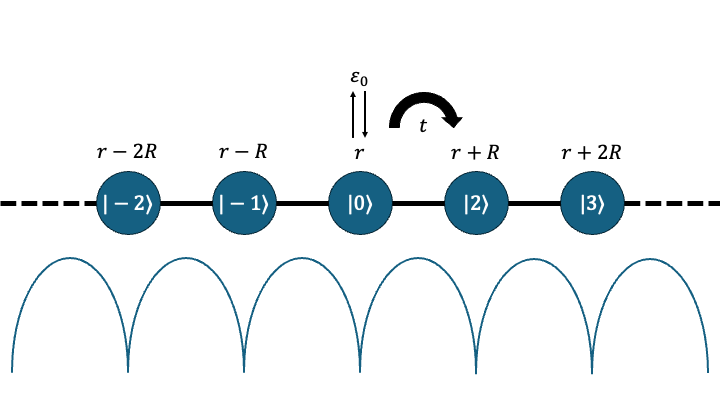
\includegraphics[max width=\linewidth]{AtomicChain.png}
    \caption{Cadena de átomos, donde los círculos representan los núcleos. En cada átomo podemos ubicar dos electrones, uno con cada spin, y pueden saltar de un elemento a otro por el término de hopping.}
    \label{fig:TBChain}
  \end{center}
\end{figure}

Estos modelos que veremos a continuación se pueden expandir facilmente a sistemas de dos o tres dimensiones. Como podemos ver, este sistema es periódico para desplazamientos de una distancia $R$, o en el caso de una red, un vector de red $\vec{R}$ o una combinación lineal de estos.

Esta periodicidad, característica de muchos sólidos cristalinos, dará lugar a muchas propiedades interesantes gracias a los resultados de estado sólido.
\subsubsection{Teorema de Bloch}

Vamos a explicar el teorema de Bloch. Consideremos un potencial periódico unidimensional, $V(x)$. Este podría ser el potencial electrostático generado por los núcleos atómicos de nuestra cadena, suponiendo a estos núcleos estáticos.

Como este potencial es periódico, debe de cumplir que $v(x) = v(x +na)$, donde $a$ es lo que se conocería como el parámetro de red. Bajo estas condiciones, el teorema de Bloch establece que la función de onda toma la forma de una onda de Bloch:
\begin{equation}
  \psi(x+a)=e^{iqa}\psi(x)
\end{equation}

Una demostración de este teorema se puede encontrar en el libro de Ashcroft y Mermin \cite{AshcroftSSP}. En el caso de una red tridimensional, el teorema de Bloch se mantiene, y podemos elegir nuestra función de onda como:
\begin{equation}
  \psi_{n\vec{k}}(\vec{r}) = e^{i\vec{k}\cdot\vec{r}}u_{n\vec{k}}(\vec{r})
\end{equation}

Donde al vector $\vec{k}$ se le conoce como el momento cristalino. Bajo estos supuestos, la ecuación de Schrödinger para la componente $u$ de la función de onda toma la siguiente forma:
\begin{equation}
  \left(-\frac{\hbar^2}{2m}(\nabla + i\vec{k})^2 + V(\vec{r})\right)u_{n\vec{k}}(\vec{r}) = \varepsilon_{n\vec{k}}u_{n\vec{k}}(\vec{r})
\end{equation}
\subsubsection{El modelo tight-binding}

La descripción que haremos del modelo de tight-binding está basada en el libro de Simons \cite{simon2013oxford}. Volvamos a la figura \ref{fig:TBChain}. Vamos a escribir nuestra función de onda en la forma de combinación lineal de orbitales atómicos. Construimos nuestra función de onda como:
\begin{equation}
  |\psi\rangle = \sum_n\phi_n|n\rangle
\end{equation}

En esta expresión, $|n\rangle$ representa la función de onda en el átomo $n$. Vamos a suponer, por simplicidad, que el solapamiento de las funciones de onda es despreciable, de forma que son ortonormales entre ellos. $\langle n|m\rangle = \delta_{nm}$. Podemos resolver, para los estados atómicos, la ecuación de Schrödinger. De este modo, tendríamos:
$$
H|\psi\rangle = \sum_m H \phi_m |m\rangle = \sum_n E \phi_{n} |n\rangle
$$

Aplicamos ahora $\langle n|$ a ambos lados. Obtenemos una ecuación:
\begin{equation}
  \sum_m H_{nm}\phi_m = E\phi_n
\end{equation}

Donde se cumple que:
\begin{equation}
  H_{nm} = \varepsilon_0\delta_{nm} + \sum_{n\neq m}\langle n | V | m \rangle
  \label{eq:hamElements}
\end{equation}

En esta expresión, $V$ es el potencial generado por los núcleos atómicos. Es decir, el potencial electrostático generado por los núcleos, que consideramos estáticos por la aproximación de Born-Oppenheimer.
$$
V = -\sum_j \frac{1}{4\pi\varepsilon_0}\frac{eq_j}{|r - R_j|^2}
$$

En nuestro caso, $\langle n | V | m \rangle$ será un término de hopping, que además restringiremos a primeros vecinos, de forma que, $\langle n | V | m\pm 1 \rangle = -t_{nm}$, donde $t_{nm}$ viene dado por la ecuación \ref{eq:hoppinFN}. De esta forma, el hamiltoniano de tight-binding con condiciones de contorno libres, para una función de onda en la base de orbitales atómicos, tiene forma de matriz tridiagonal.
\begin{equation}
  H_{nm} = \left(\begin{array}{ccccc}
    \varepsilon_0 & -t & 0 & \ldots & 0 \\
    -t & \varepsilon_0 & -t & \ldots & 0 \\
    0 & -t & \varepsilon_0 & \ldots & 0 \\
    \vdots & \vdots & \vdots & \ddots & \vdots \\
    0 & 0 & 0 & \ldots & \varepsilon_0
  \end{array}\right)
\end{equation}

Si imponemos a nuestra cadena condiciones periódicas, podemos encontrar las bandas de energía utilizando el teorema de Bloch. Notemos que esta matriz no tiene condiciones periódicas, si se las añadimos deberíamos de añadir un término de hopping, $t$, en las esquinas donde hay $0$. En este caso, el más sencillo, cada núcleo representa su propia celda unidad. Para resolver problemas de tight-binding, solemos suponer una solución de los coeficientes de la forma $\phi_n = \frac{e^{-ikna}}{\sqrt{N}}$ donde $a$ es el parámetro de red, o la distancia entre celdas unidad.

Gracias al teorema de Bloch, únicamente hay que resolver la ecuación de Schrödinger para una celda unidad, luego, si nos situamos en una celda unidad con $n$ fijo y aplicamos la ecuación de Schrödinger, con los elementos de $H$ tomando la forma de la ecuación \ref{eq:hamElements}, tendremos una expresión con la siguiente forma:
$$
-t(e^{-ik(n+1)a} + e^{-ik(n-1)a}) + \varepsilon_0e^{-ikna} = Ee^{-ikna}
$$

Y podemos despejar una expresión para la banda de energías permitidas, de la forma $E(k)$, que toma la siguiente ecuación:
\begin{equation}
  E = \varepsilon_0 - 2tcos(ka)
  \label{eq:bandasTB}
\end{equation}

Los niveles de energía siguen siendo discretos, pero ahora son tan densos que se forman las bandas. Lo que nos quiere decir esta descripción, es que $\vec{k}$ es ahora un buen número cuántico, que nos va a ser de utilidad para describir las propiedades de nuestro sistema.

La posición de estas bandas y su posición relativa a la energía de Fermi, van a definir las propiedades de conducción de cada material.  Dependerán de la geometría del mismo,  de las condiciones del hopping y otros términos como la cantidad de orbitales que consideremos por átomo. En nuestro caso, nos vamos a quedar con el modelo de tight-binding más simple, por lo que tendremos una única banda con la forma que aparece en la figura \ref{fig:bandaTB}.
\begin{figure}[h!]
  \begin{center}
    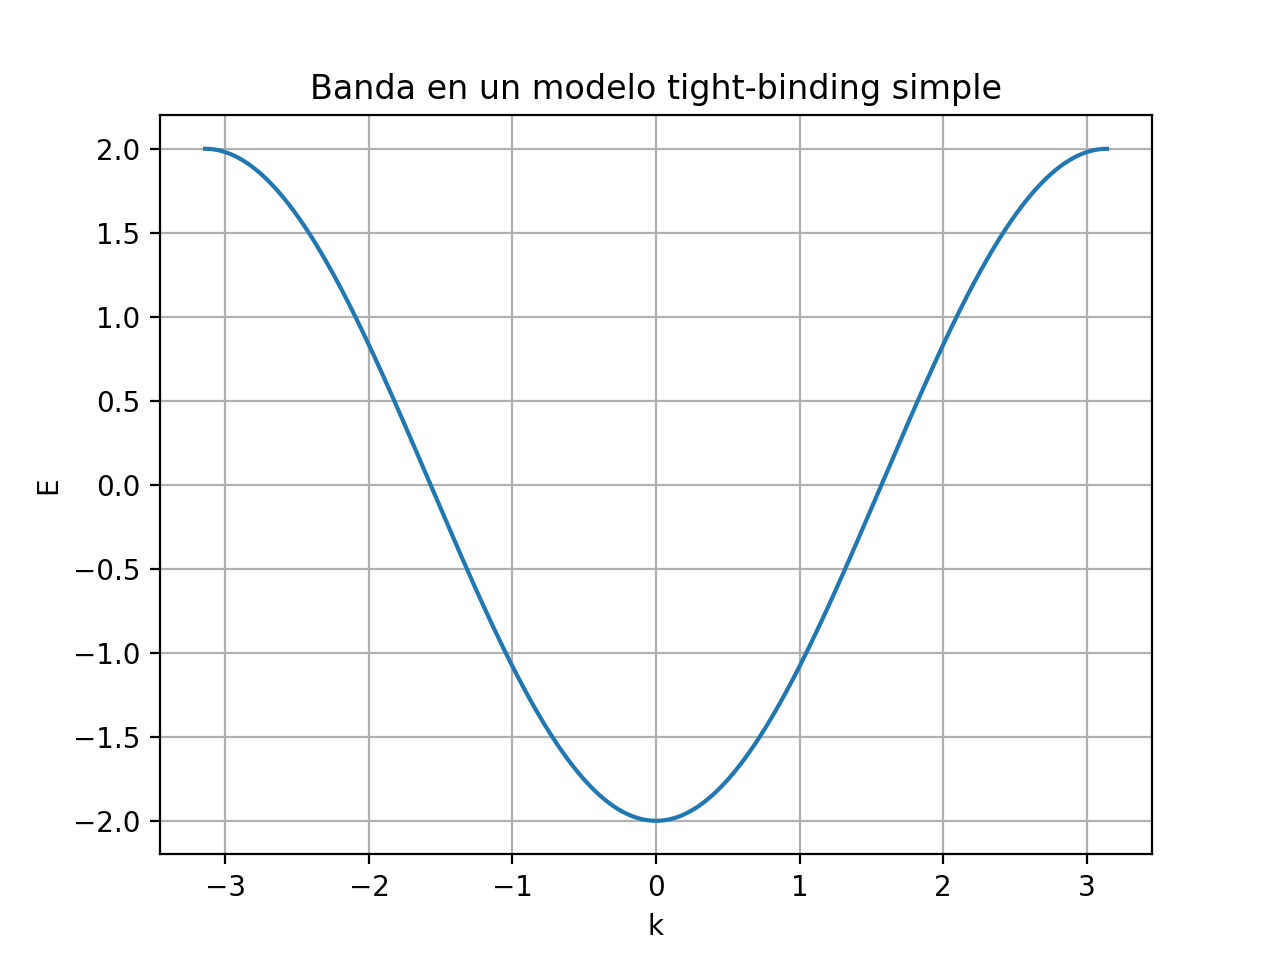
\includegraphics[max width=\linewidth]{BandTB.png}
    \caption{La única banda que aparece en el sistema de tight-binding que hemos considerado. Estamos considerando $\varepsilon_0 = 0$ y $t = 1$.}
    \label{fig:bandaTB}
  \end{center}
\end{figure}

Vamos a definir a continuación la densidad de estados (en inglés la DOS). Es una función que define la probabilidad de encontrar una partícula a una energía dada, y se construye siguiendo la expresión:
\begin{equation}
  N = \int_0^{E_F} g(E) \, dE
\end{equation}

Además, en esta definición ya aparece otra cantidad importante, que es la energía de Fermi. Representa una energía a la que, si integramos nuestra densidad de estados, deben de aparecer todos los electrones del sistema, es decir, todos los niveles de energía por debajo de la energía de Fermi están ocupados y por encima desocupados.

Queremos encontrar la densidad de estados para el sistema de tight-binding que hemos considerado. Esto puede hacerse de la siguiente manera:
$$
g(E) = \frac{\partial N}{\partial E} = \frac{\partial N}{\partial k}\frac{\partial k}{\partial E} = \frac{\partial N}{\partial k}\left|\frac{\partial E}{\partial k}\right|^{-1}
$$

Con la expresión anterior es fácil calcular la densidad de estados:
\begin{equation}
  g(E) = \frac{1}{\pi}\frac{1}{|\sin(k(E)a)|}
\end{equation}

Ahora bien, vemos que hay puntos de esta función en los que el denominador se anula, estos puntos se conocen como las singularidades de Van-Hove, y van a causar divergencias en la densidad de estados.

Pero esta densidad de estados no está escrita en función de la energía, para ello deberemos de usar la relación que calculamos antes para las bandas (ecuación \ref{eq:bandasTB}) para hacer un cambio de variable, es sencillo entonces ver que:
\begin{equation}
  g(E) = \frac{1}{\pi at}\frac{1}{\sqrt{1-\left(\frac{E}{2t}\right)^2}}
\end{equation}

Ahora sí, podemos ver representada esta densidad de estados en la figura \ref{fig:dosTB}, donde se observan los picos de la divergencia, y el resto de la densidad aplanada.
\begin{figure}[h!]
  \begin{center}
    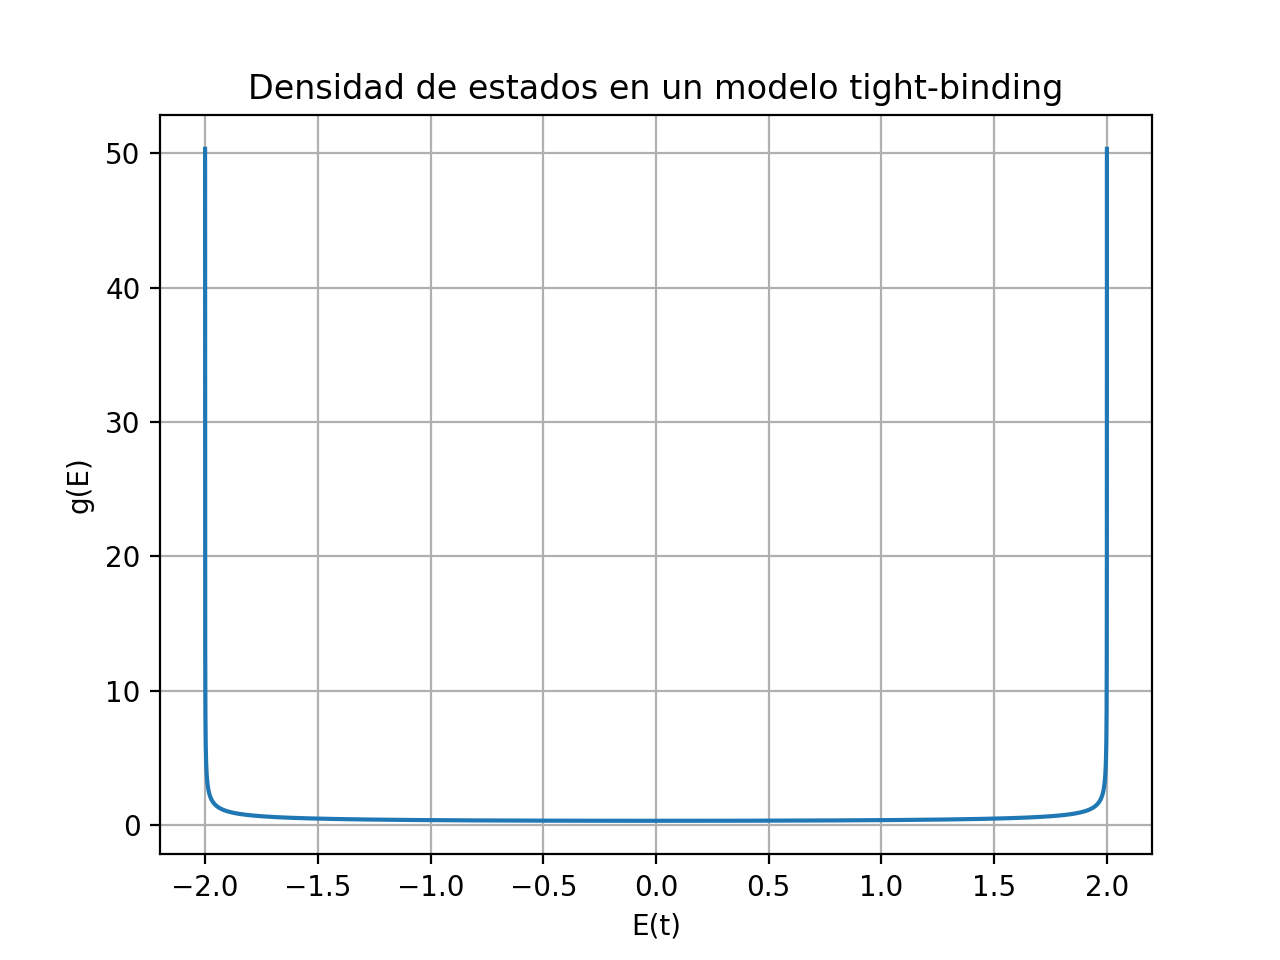
\includegraphics[max width=\linewidth]{DosTB.png}
    \caption{Densidad de estados en un modelo sencillo de tight-binding. Se puede observar el efecto de las singularidades de Van-Hove. En este caso, nuestra energía de Fermi está en $E_F = 0$, situándose en el centro y los fermiones se ubican en los niveles más bajos de energía. Nuevamente consideramos $\varepsilon_0 = 0$ y $t = 1$.}
    \label{fig:dosTB}
  \end{center}
\end{figure}

Ahora que entendemos al completo un mecanismo de tight-binding, podemos seguir avanzando para añadir interacciones de dos partículas. Sin embargo, para ello será conveniente introducir el formalismo de segunda cuantización al trabajo que hemos hecho hasta ahora, es por ello que primero haremos eso.

En el siguiente subapartado, vamos a escribir brevemente el hamiltoniano de tight-binding en la forma de segunda cuantización, tal y como describimos en la sección \ref{sec:secondQuantized}. De este modo, podremos comenzar a familiarizarnos con los hamiltonianos en esta forma.
\subsubsection{Tight-binding en segunda cuantización}

Antes de adentrarnos a escribir el hamiltoniano en segunda cuantización, vamos a dar una descripción del hopping de una forma más general. Esto será conveniente a la hora del desarrollo computacional. La matriz de hopping no es más que una matriz que define el hopping con elementos $t_{ij}$, por ejemplo, en nuestro caso, si consideramos condiciones periódicas e interacción a primeros vecinos, la matriz toma la forma:
\begin{equation}
  t_{ij} = \left(\begin{array}{ccccc}
    \varepsilon_0 & t & 0 & \ldots & t \\
    t & \varepsilon_0 & t & \ldots & 0 \\
    0 & t & \varepsilon_0 & \ldots & 0 \\
    \vdots & \vdots & \vdots & \ddots & \vdots \\ 
    t & 0 & 0 & \ldots & \varepsilon_0
  \end{array}\right)
\end{equation}

Como vemos, aquí aparece el hopping en las esquinas debido a las condiciones periódicas del sistema y a primeros vecinos. Pero con esta matriz, podríamos generalizar el hopping a cualquier número de vecinos de una forma sencilla, con o sin condiciones de contorno periódicas.

Recordemos la ecuación \ref{eq:sqOperators} para escribir operadores en segunda cuantización para fermiones, que será nuestro caso de ahora en adelante, pues nos interesan los electrones. Podemos escribir nuestro hamiltoniano de manera sencilla utilizando lo que hemos visto tal que:
\begin{equation}
  \hat{H} = \sum_{i, j, \sigma}t_{ij}c_{i, \sigma}^{\dagger} c_{j, \sigma}
\end{equation}

Donde $\sigma$ representa una suma sobre los dos posibles spines de un electrón. Como se puede ver, resulta un hamiltoniano sencillo.
\subsection{El modelo de Hubbard}

Vamos a introducir, a continuación, el hamiltoniano de Hubbard, que se puede ver en la referencia \cite{MielkeHubbard}. Este hamiltoniano ya ha aparecido con anterioridad:
\begin{equation*}
  \recallLabel{eq:hubbardHam}
\end{equation*}

Este modelo puede escribirse en forma de matriz, sin embargo, el tamaño del espacio es mucho más grande que en el caso del tight-binding. Además, aparece una forma de matriz dispersa, que es mucho más complicada de diagonalizar, es por ello que recurriremos a algoritmos numéricos para obtener los autovalores y autoestados del hamiltoniano.

El hamiltoniano presenta una contribución $U$ a la energía cuando haya dos partículas juntas en un mismo estado atómico. Más adelante veremos que este fenómeno será de importancia. Un material que siga el modelo de Hubbard, presentará un cambio en sus propiedades. El término de interacción pretende modelar la interacción electrostática entre dos electrones en un mismo sitio, pero de una forma sencilla, como una constante.

Se demuestra teóricamente en la referencia \cite{MielkeHubbard}, que el hamiltoniano de Hubbard presenta una simetría gauge, una simetría de spin, de red y una simetría frente a transformaciones a huecos para el caso del semillenado. En dicha referencia, aparecen también algunos teoremas que cumple el modelo, cito a continuación alguno de los más relevantes:
\begin{enumerate}
  \item \textbf{Teorema de Lieb, 1989:} el hamiltoniano de Hubbard con $U_x < 0$, con un número de partículas par, presenta un único estado fundamental, de spin total $S = 0$.
  \item \textbf{Corolario:} El hamiltoniano de Hubbard, con interacción $U_x > 0$ y un número de partículas con semillenado, el estado fundamental es único en el subespacio $S_z = 0$ con spin total $S = \frac{1}{2}\left||A| - |B|\right|$.
\end{enumerate}

El teorema de Lieb es interesante, puesto que nos servirá más adelante para comprobar que nuestros resultados andan bien encaminados, y es otra forma de obtener información del estado fundamental sin calcularlo explícitamente.

El corolario que aparece también es interesante, nos habla de redes bipartitas. En nuestro caso, podemos considerar que tenemos nuestra red dividida en dos redes iguales, y en este caso, el spin total de cada red es el mismo, haciendo que se anulen.
\subsection{Funciones de Green}

A continuación, introduciremos las funciones de Green \cite{fetter1971quantum}. Estas funciones nos van a permitir estudiar con más comodidad las propiedades de sistemas de muchas partículas. Por ejemplo, la función de Green de una partícula nos permite conocer toda la información del espectro de excitaciones a partir del estado fundamental, esta es:
\begin{equation}
  iG_{\alpha\beta}(\vec{x}t, \vec{x}'t') = \frac{\left\langle\Psi_0|T\left(\hat{\psi}_{H\alpha}(\vec{x}t)\hat{\psi}^{\dagger}_{H\beta}(\vec{x}'t')\right)|\Psi_0\right\rangle}{\langle\Psi_0|\Psi_0\rangle}
  \label{eq:GreenFunction}
\end{equation}

En esta expresión hay mucho que descomponer. $|\Psi_0\rangle$ es el estado fundamental en la representación de Heisenberg del sistema interactuante, satisfaciendo $\hat{H}|\Psi_0\rangle = E|\Psi_0\rangle$ y $\hat{\psi}_{H\alpha}(\vec{x}t)$ es un operador en la representación de Heisenberg dado por:
\begin{equation}
  \hat{\psi}_{H\alpha} = e^{i\frac{\hat{H}}{\hbar}t}\hat{\psi}_{\alpha}(\vec{x})e^{-i\frac{H}{\hbar}t}
\end{equation}

En esta definición, los índices $\alpha$ y $\beta$ son las componentes del operador de campo. Estos índices pueden tomar dos valores para los fermiones de spin $\frac{1}{2}$, mientras que no hay índices para bosones de spin cero, puesto que dichos sistemas se describen por un campo de un componente.

Todo esto se puede relacionar con la teoría cuántica de campos, como ya hemos mencionado más arriba. Estos operadores de campo actúan como una proyección en el espacio de posiciones de los operadores de creación y destrucción. Crean (o aniquilan) partículas en una posición.

Por otro lado, $T$ representa una ordenación temporal. En nuestro sistema no importa mucho, porque no tenemos una dependencia explícita del hamiltoniano con el tiempo, pero si la tuviésemos, $T$ tomaría la siguiente forma:
\begin{equation}
  T\left(\hat{\psi}_{H\alpha}(\vec{x}t)\hat{\psi}^{\dagger}_{H\beta}(\vec{x}'t')\right) = \left\{\begin{array}{cc}
      \hat{\psi}_{H\alpha}(\vec{x}t)\hat{\psi}^{\dagger}_{H\beta}(\vec{x}'t') & t > t' \\
      \pm\hat{\psi}_{H\alpha}^{\dagger}(\vec{x}'t')\hat{\psi}_{H\beta}(\vec{x}t) & t' > t
  \end{array}\right.
\end{equation}

Donde el cambio de signo sólo sucede en el caso de fermiones para la segunda ecuación. De forma general, el producto $T$ de varios operadores los ordena de derecha a izquierda, en orden ascendente temporal y añade un factor $(-1)^P$, donde $P$ es el número de intercambios de operadores de fermiones respecto al orden original.

De esta forma, la función de Green aparece como el valor esperado de operadores de campo. Si el hamiltoniano $\hat{H}$ es independiente del tiempo, $G$ únicamente depende de la diferencia de tiempos.
$$
iG_{\alpha\beta}(\vec{x}t, \vec{x}'t') = \left\{\begin{array}{cc}
    e^{i\frac{E}{\hbar}(t-t')}\frac{\left\langle\Psi_0\left|\hat{\psi}_{\alpha}(\vec{x})e^{-i\frac{\hat{H}}{\hbar}(t-t')}\hat{\psi}^{\dagger}_{\beta}(\vec{x'})\right|\Psi_0\right\rangle}{\langle\Psi_0|\Psi_0\rangle} & t>t' \\
    \pm e^{-i\frac{E}{\hbar}(t-t')}\frac{\left\langle\Psi_0\left|\hat{\psi}^{\dagger}_{\alpha}(\vec{x})e^{i\frac{\hat{H}}{\hbar}(t-t')}\hat{\psi}_{\beta}(\vec{x'})\right|\Psi_0\right\rangle}{\langle\Psi_0|\Psi_0\rangle} & t'>t
\end{array}\right.
$$

Podemos definir las funciones de Green avanzada y retardada, usando el anticonmutador de los operadores de campo. en vez del operador de ordenación temporal. La función retardada valdrá cero para $t' > t$. La avanzada será cero si $t > t'$.
\subsubsection{Aplicaciones de las funciones de Green}

Una vez hemos obtenido la función de Green, podemos hacer muchas cosas con ellas. En esta sección vamos a presentar algunos resultados. Estas funciones son interesantes a la hora de calcular los diagramas de Feynman debido a que las reglas son más sencillas para ellas.

Además, podemos obtener algunas cantidades interesantes de nuestro sistema conociendo únicamente el estado fundamental:
\begin{enumerate}
  \item El valor esperado de un operador de una única partícula en el estado fundamental.
  \item La energía del estado fundamental del sistema.
  \item El espectro de excitaciones del sistema.
\end{enumerate}

A continuación, vamos a intentar obtener el valor de la densidad de estados a partir de las funciones de Green. Esta cantidad será de nuestro interés para el resto del trabajo, pues nuestros cálculos girarán en torno a la misma.

Para comenzar con el desarrollo, debemos de introducir los operadores de Green en la representación $\omega$-Lehman:
\begin{equation}
  \begin{array}{ccc}
    \hat{G}^+(\omega) = \lim_{\eta\to 0^+}\frac{1}{\omega - H + E_0 + i\eta} & \hspace{0.1\linewidth} & \hat{G}^-(\omega) = \lim_{\eta\to 0^+}\frac{1}{\omega + H - E_0 - i\eta}
  \end{array}
\end{equation}

Y las funciones de Green son:
\begin{equation}
  \begin{array}{cc}
    G^+(\tau, \tau', \omega) = \langle\psi_0|c_{\tau}\hat{G}^+c_{\tau}^{\dagger}|\psi_0\rangle & G^-(\tau, \tau', \omega) = \langle\psi_0|c_{\tau}^{\dagger}\hat{G}^-c_{\tau}|\psi_0\rangle
  \end{array}
\end{equation}

Vamos a escribir la función de Green, $G^+$, en el espacio de posiciones, esto sería:
$$
G^+(\vec{R}, \vec{R}', \omega) = \left\langle\psi_0\left| c_{\vec{R}}\frac{1}{\omega - H + E_0 + i\eta}c_{\vec{R}}^{\dagger}\right|\psi_0\right\rangle
$$

Tomemos la transformada de Fourier de los operadores de creación y destrucción en la expresión anterior, es decir, vamos a sustituir por los siguientes valores:
$$
\begin{array}{ccc}
  c_{\vec{R}} = \sum_{\vec{k}}\sqrt{\frac{1}{V}}e^{i\vec{k}\cdot\vec{R}}c_{\vec{k}} & \hspace{0.1\linewidth} & c_{\vec{R}'}^{\dagger} = \sum_{\vec{k}'}\sqrt{\frac{1}{V}}e^{-i\vec{k}'\cdot\vec{R}'}c_{\vec{k}'}^{\dagger}
\end{array}
$$

Si sustituimos estos operadores de creación y destrucción en la expresión anterior tendremos lo siguiente:
$$
G^+(\vec{R}, \vec{R}', \omega) = \frac{1}{V}\sum_{\vec{k}, \vec{k}'}e^{i\left(\vec{k}\cdot\vec{R} - \vec{k}'\cdot\vec{R}'\right)}G^+(\vec{k}, \vec{k}', \omega)
$$

Tenemos que ver la forma que tiene $G^+(\vec{k}, \vec{k}', \omega)$ para continuar con el desarrollo. Vamos a explicitarlo, esto sería:
$$
G^+(\vec{k}, \vec{k}', \omega) = \left\langle\psi_0\left| c_{\vec{k}}\frac{1}{\omega - H + E_0 + i\eta}c_{\vec{k}'}^{\dagger}\right|\psi_0\right\rangle
$$

Ahora bien, estamos trabajando en una estructura de bandas, por lo que $\psi_0$ tendrá vacíos todos los niveles por encima de la energía de Fermi, es decir, sólo podemos crear partículas con energía superior al nivel de Fermi, puesto que todos los niveles por debajo estarán llenos. Por ende, tendremos que:
$$
Hc_{\vec{k}'}^{\dagger}|\psi_0\rangle = \left(E_0 + \varepsilon_{\vec{k}'}\right)c_{\vec{k}'}^{\dagger}|\psi_0\rangle
$$

Es decir, es la energía del estado fundamental, más la de una partícula en $\vec{k}'$, siempre que se cumpla la condición de que $\varepsilon_{\vec{k}'} > \varepsilon_F$, para asegurar que estamos creando partículas por encima del nivel de Fermi. Podremos ver que:
$$
G^+(\vec{k}, \vec{k}', \omega) = \delta_{\vec{k}\vec{k}'}\left\{\begin{array}{cc}
  0 & \varepsilon_{\vec{k}'} < \varepsilon_F \\
  \frac{1}{\omega - \varepsilon_{\vec{k}'} + i\eta} & \varepsilon_{\vec{k}'} > \varepsilon_F
\end{array}\right.
$$

Si volvemos a la expresión anterior, podemos suplir la condición gracias a la delta que aparece en frente de la función de Green, obteniendo que:
$$
G^+(\vec{R}, \vec{R}', \omega) = \frac{1}{V}\sum_{\vec{k}}e^{i\vec{k}\cdot\left(\vec{R} - \vec{R}'\right)}G^+(\vec{k}, \vec{k}, \omega)
$$

De manera similar para la función $G^-$, obtenemos que:
$$
G^-(\vec{R}, \vec{R}', \omega) = \frac{1}{V}\sum_{\vec{k}}e^{i\vec{k}\cdot\left(\vec{R} - \vec{R}'\right)}G^-(\vec{k}, \vec{k}, \omega)
$$

Obteniendo que para los valores diagonales:
$$
G^{\pm}(\vec{R}, \vec{R}, \omega) = \frac{1}{V}G^{\pm}(\vec{k}, \vec{k}, \omega) = \frac{1}{V}\sum_{\vec{k}}\frac{\pm 1}{\omega - \varepsilon_{\vec{k}} \pm i\eta}
$$

Donde este último término viene de dar la misma expresión para $G^-$ que hicimos en el caso de $G^+$, pero en este caso debemos destruir partículas por debajo del nivel de Fermi, jugando un poco con los denominadores podemos llegar a esta expresión.

Dentro de la suma hemos obtenido una función lorentziana, que en el límite $\eta\to 0^+$ se convierte en una delta, por lo que nos queda finalmente que la parte imaginaria es:
\begin{equation}
  \begin{split}
    Im(G^+(\vec{R}, \vec{R}, \omega)) = -\pi\frac{1}{V}\sum_{\vec{k}, \varepsilon_{\vec{k}}\gtrless\varepsilon_F}\delta(\omega - \varepsilon_{\vec{k}}) = -\pi DOS(\omega) \implies \\ -\frac{1}{\pi}Im\left(G^+\left(\vec{R}, \vec{R}, \omega\right)\right) = DOS\left(\omega\right)
  \end{split}
\end{equation}

Si sustituimos por el valor absoluto de la parte imaginaria, podemos usar cualquiera de las dos funciones de Green, si no, nos restringimos al valor de la función $G^+$, puesto que la densidad de estados debe de ser positiva.

Lo que obtenemos es la densidad de estados ocupados o desocupados, en función de que función de Green estemos utilizando. Observamos que la densidad de estados se compondrá de picos centrados en las energías ocupadas (o desocupadas). Con lo que nos da importante información sobre los niveles energéticos del sistema.

En las siguientes secciones del trabajo haremos una representación de la densidad de estados, sumando los ocupados y desocupados, para obtener algo que nos represente la densidad completa. Veremos que la forma de diferenciar a qué tipo pertenece cada una veremos la posición de la energía de Fermi.

Las funciones de Green tienen muchas más aplicaciones. Aquí hemos trabajado con la función de Green de una partícula, pero también existen las de dos o más partículas. Son importantes en otras situaciones, por ejemplo, nos podrían dar una idea de la densidad de pares up-down de nuestro sistema, entre otras cosas. Cabe mencionar que no hemos añadido el spin en este desarrollo, pero su adición es directa.
\newpage
\section{El algoritmo de Lanczos}

Nuestro objetivo es obtener propiedades de los sistemas que siguen el hamiltoniano de Hubbard (\ref{eq:hubbardHam}). Se puede tomar el camino de las aproximaciones y las simplificaciones, pero en nuestro caso vamos a tomar el camino de las soluciones de forma numérica.

El modelo de Hubbard no tiene soluciones analíticas exactas para un número general de dimensiones. Además, el estudio numérico del modelo está limitado por la dimenisionalidad del espacio en el que trabaja el algoritmo de Lanczos, derivando en un gran coste en memoria. Este espacio se conoce como espacio de Krylov, y tiene la siguiente dimensionalidad:
$$
dimn = \left(\begin{array}{c}
  N \\
  N_{\uparrow}
\end{array}\right)\left(\begin{array}{c}
  N \\
  N_{\downarrow}
\end{array}\right)
$$

Por lo que para ordenadores modernos, una cadena relativamente no muy grande, tiene un coste en memoria muy alto en una resolución numérica exacta (cosa que podríamos hacer con el algoritmo de Lanczos). Es debido a este alto coste, que en este trabajo vamos a utilizar el algoritmo de Lanczos modificado, pero para ello, primero debemos conocer el algoritmo de Lanczos.

Es evidente que el hamiltoniano de Hubbard (\ref{eq:hubbardHam}) no tiene una representación matricial evidente o sencilla. Quizás una matriz dispersa pueda representarlo, pero sigue siendo complicado obtener sus autovalores y autovectores. Todo sería mucho más sencillo si pudieramos representar el hamiltoniano como una matriz tridiagonal.

Aquí aparece el algoritmo de Lanczos, siguiendo la referencia \cite{RevModPhys.66.763}, encontraremos el algoritmo de Lanczos. Este es un algoritmo de diagonalización exacto que nos permite obtener una base en la que un hamiltoniano cualquiera tiene forma de matriz tridiagonal.
\subsection{Descripción del método}

Para comenzar, vamos a elegir un vector arbitrario $|\phi_0\rangle$ en nuestro espacio de Hillbert. Si se usa el modelo para obtener el estado fundamental del sistema, necesitaríamos un overlap entre nuestro vector $|\phi_0\rangle$ y el estado fundamental del sistema $|\psi_0\rangle$ no nulo. Si conocemos alguna información del estado fundamental podemos facilitarnos este trabajo. En cualquier otro caso, simplemente tomaremos un vector aleatorio. De esta forma, vamos a ir construyendo iterativamente los vectores de la base.
\begin{equation}
|\phi_1\rangle = \hat{H}|\phi_0\rangle - \frac{\langle\phi_0|\hat{H}|\phi_0\rangle}{\langle\phi_0|\phi_0\rangle}|\phi_0\rangle
\end{equation}

Podemos ir construyendo una base de manera recurrente, si tomamos $n = 0, 1, 2, \ldots$, tendremos que los vectores son de la forma:
\begin{equation}
    |\phi_{n+1}\rangle = \hat{H}|\phi_n\rangle - a_n|\phi_n\rangle - b_n^2|\phi_{n-1}\rangle
\end{equation}

Donde, los coeficientes vienen dados por las siguientes ecuaciones:
\begin{equation}
    \begin{array}{ccc}
        a_n = \frac{\langle\phi_n|\hat{H}|\phi_n\rangle}{\langle\phi_n|\phi_n\rangle} & \hspace{0.25\linewidth} & b_n^2 = \frac{\langle\phi_n|\phi_n\rangle}{\langle\phi_{n-1}|\phi_{n-1}\rangle}
    \end{array}
\end{equation}

Donde también suplimos la condición de $b_0 = 0$. De este modo la fórmula queda completa, si definimos nuestra base de este modo, encontraremos que el hamiltoniano tridiagonal tiene la siguiente forma:
\begin{equation}
    H = \left(\begin{array}{ccccc}
        a_0 & b_1 & 0 & 0 & \ldots \\
        b_1 & a_1 & b_2 & 0 & \ldots \\
        0 & b_2 & a_2 & b_3 & \ldots \\
        0 & 0 & b_3 & a_3 & \ldots \\
        \vdots & \vdots & \vdots & \vdots & \ddots
    \end{array}\right)
\end{equation}

Una vez tenemos esta matriz tridiagonal, cualquier algoritmo típico para obtener autovalores y autovectores de matrices es suficiente para calcular la diagonalización de la matriz.
\subsection{El algoritmo modificado}

Como hemos mencionado más arriba, la dimensión del método de Lanczos, en lo que se conoce como el espacio de Krylov, crece demasiado rápido, y guardar todos los vectores en memoria no es muy conveniente. Sin embargo, el método de Lanczos nos permite obtener buena información sobre el estado fundamental sin necesidad de obtener el espacio completo.

Esta afortunada propiedad, nos motiva a modificar el método de Lanczos de una manera iterativa, de forma que haciendo un número $l$ de iteraciones de Lanczos en cada repetición, podemos ir convergiendo al estado fundamental.

El procedimiento es el siguiente:
\begin{enumerate}
  \item Tomar un vector, $\phi_0$, inicial arbitrario.
  \item Aplicar un número $l$ de iteraciones de Lanczos y obtener el autovalor mínimo del hamiltoniano $l \times l$, $E_0$, y su autovector correspondiente, $\psi_0$.
  \item Obtenemos un nuevo vector inicial, $\psi_0$. Si la energía cumple la condición de convergencia, tenemos nuestro estado fundamental y energía. Si no, almacenamos en memoria $E_0$ y repetimos el paso 2 pero con el nuevo vector $\psi_0$ como vector inicial.
\end{enumerate}

Este método no sólo nos permite obtener el estado fundamental con rapidez, si no que además genera una función de Green mucho más limpia una vez la calculemos.

\subsection{Valores esperados en el estado fundamental}

Como ya hemos hablado con anterioridad, resulta de gran interés obtener las funciones de Green. Los valores de esta función también se pueden obtener con el algoritmo de Lanczos, el método general para cualquier operador viene expresado en la referencia \cite{RevModPhys.66.763}. Sin embargo, para la función de Green de una partícula he decidido tomar la descripción dada por Greene y et.al. en su artículo \cite{GreeneDiniz2024}.

Usualmente vamos a estar interesados en obtener expresiones de la forma:
$$
I(\omega) = -\frac{1}{\pi}Im\left(\left\langle\psi_0 \left|\hat{O}^{\dagger}\frac{1}{\omega + E_0 + i\epsilon - \hat{H}}\hat{O}\right|\psi_0\right\rangle\right)
$$

Si obtenemos los coeficientes de Lanczos con la función de onda inicial $|\phi_0\rangle = \hat{O}|\psi_0\rangle$, donde $|\psi_0\rangle$ es el estado fundamental del sistema, entonces, estos valores serán:
\begin{equation}
  I(\omega) = -\frac{1}{\pi}Im\left( \frac{\left\langle\psi_0\left| \hat{O}^{\dagger}\hat{O}\right|\psi_0\right\rangle}{\omega + E_{GS} - a_0 - \frac{b_1^2}{\omega + E_{GS} - a_1 - \frac{b_2^2}{\omega + E_{GS} - a_2 - \ldots}}}\right)
\end{equation}

Donde vamos a desplazar $\omega$ para desplazar los polos al plano imaginario. Tomaremos que $\omega = \omega_0 + i\eta$.

Por lo que, nuestro programa consistirá en una primera ejecución del algoritmo de Lanczos para obtener el estado fundamental, y las ejecuciones subsecuentes para obtener los operadores que queramos.
\subsubsection{Función de Green de una partícula}

En el caso de la función de Green de una partícula, vamos a tener expresiones en las que $\hat{O} = c_{i\sigma}$ para partículas u $\hat{O} = c_{i\sigma}^{\dagger}$ para huecos. La función de Green tendrá dos partes: la asociada a los huecos y la asociada a las partículas. Si queremos una representación de la densidad de estados al completo deberemos de calcular ambas, pero si sólo nos interesan los estados ocupados (o desocupados), únicamente calcularemos la función de Green para partículas (o huecos).

Nos interesa la densidad de estados. Esta se relaciona con la función de Green numérica por:
\begin{equation}
  DOS = -\frac{1}{\pi}tr\left(Im\left(G(\omega)\right)\right)
\end{equation}

Vamos a seguir el desarrollo de \cite{GreeneDiniz2024}. Este nos permite calcular la densidad de estados al completo. Para hacer esto, debemos de realizar, por cada elemento de la traza, $G_{i,i}$, dos iteraciones del algoritmo de Lanczos (una para partículas y otra para huecos).

Sin embargo, no partiremos del estado fundamental para iterar Lanczos. Deberemos de tomar como vector inicial, para cada caso, uno de los siguientes estados:
\begin{equation}
  \begin{array}{ccc}
    \left|\psi_{i, i}^{(h)}\right\rangle = \frac{c_{i\sigma}^{\dagger}\left|\psi_0\right\rangle}{\sqrt{n_{i, i}^{(p)}}} & \hspace{0.15\linewidth} & \left|\psi_{i, i}^{(p)}\right\rangle = \frac{c_{i\sigma}\left|\psi_0\right\rangle}{\sqrt{n_{i, i}^{(h)}}}
  \end{array}
\end{equation}

En este caso, $|\psi_0\rangle$ representa la función de onda del estado fundamental, que podemos obtener mediante el algoritmo de Lanczos anteriormente descrito. Los valores de los denominadores son:
\begin{equation}
  \begin{array}{ccc}
    n_{i, i}^{(p)} = \left\langle\psi_0\left| c_{i\sigma}^{\dagger}c_{i\sigma}\right|\psi_0\right\rangle & \hspace{0.15\linewidth} & n_{i, i}^{(h)} = \left\langle\psi_0\left| c_{i\sigma}c_{i\sigma}^{\dagger}\right|\psi_0\right\rangle
  \end{array}
\end{equation}

Aplicamos el algoritmo de Lanczos a cada uno de estos estados inciales y obtenemos sus correspondientes coeficientes. Aparecerá la función de Green, pero en forma de fracción continuada y para una partícula:
\begin{equation}
  \begin{split}
    G_{i, i} = \frac{n_{i, i}^{(h)}}{\omega + E_0 - a_0^{(h)} - \frac{\left(b_1^{(h)}\right)^2}{\omega + E_0 - a_1^{(h)} - \frac{\left(b_2^{(h)}\right)}{\omega + E_0 - a_2^{(h)} - \ldots}}} + \\ + \frac{n_{i, i}^{(p)}}{\omega - E_0 + a_0^{(p)} - \frac{\left(b_1^{(p)}\right)^2}{\omega - E_0 + a_1^{(p)} - \frac{\left(b_2^{(p)}\right)}{\omega - E_0 + a_2^{(p)} - \ldots}}}
  \end{split}
  \label{eq:greenLanczos}
\end{equation}

El cálculo de los elementos extradiagonales es similar, pero debemos de tomar combinaciones lineales de los operadores de creación y destrucción  para los vectores iniciales.
\begin{equation}
  \left|\psi_{i\neq j}^{(p)}\right\rangle = \frac{\left(c_i + c_j\right)|\psi_0\rangle}{\sqrt{n^{(p)}_{i\neq j}}}
\end{equation}

Lo que calcularíamos ahora con la ecuación \ref{eq:greenLanczos}, sería un elemento, que denominaremos, $G_{i, j}^L$, si queremos obtener los verdaderos valores debemos de aplicarles una transformación:
\begin{equation}
  G_{i\neq j} = \frac{1}{2}\left(G_{i, j}^L - G_{i, i} - G_{j, j}\right)
\end{equation}
\newpage
\section{Desarrollo}

Para este trabajo, se ha procedido a la implementación del algoritmo de Lanczos para el hamiltoniano de Hubbard en cadenas pequeñas. El algoritmo, descrito anteriormente, nos servirá para obtener la información necesaria del estado fundamental, así como la densidad de estados y otros valores interesantes relativos a las funciones de Green.

Todo el código generado para este trabajo se podrá encontrar en mi perfil de GitHub, junto al código Latex del documento final. \href{https://github.com/luisgotsky}{[ENLACE]}
\subsection{Tratamiento de datos}

Lo primero que habrá que hacer, es encontrar una representación de las funciones de onda que nos permita trabajar de forma satisfactoria pero sin saturar la memoria. En nuestro caso, estamos considerando funciones de onda en la base $LCAO$, que son de la forma:
$$
|\psi\rangle = \sum_i \phi_i|i, \sigma\rangle
$$

Donde $|i\rangle$ representa la función de onda asociada a un núcleo en la posición $i$ con un electrón de spin $\sigma$. En nuestro caso, una representación más adecuada de la función de onda sería algo de la siguiente forma:
$$
|\psi\rangle = \alpha_1|\uparrow\downarrow, \uparrow, \downarrow, \downarrow, \ldots, \uparrow\rangle + \alpha_2|0, \uparrow\downarrow, 0, \uparrow\downarrow, \ldots, 0\rangle + \ldots
$$

Básicamente, es una combinación lineal de cadenas, donde es bastante directo ver que la posición en el ket es la posición en la cadena atómica. Además, estos estados son ortonormales, puesto que en segunda cuantización se cumple que:
$$
\langle\psi_1|\psi_2\rangle = \sum_{i, j}\alpha_i\beta_j\langle 0| c_{i1}c_{i2}\ldots c_{j1}^{\dagger}c_{j2}^{\dagger}|0\rangle
$$

Y la única forma en que el bra-ket no sea cero es que los operadores de destrucción destruyan lo que crean los operadores de creación. Las reglas de producto por un escalar y suma de vectores siguen idénticas a las de cualquier vector.

Podremos codificar las posiciones de cada spin con dos cadenas binarias, es decir, que tendremos:
$$
\begin{array}{ccc}
  |\psi_{i\uparrow}\rangle = |1, 0, 0, 1, \ldots, 0\rangle = |x\rangle_n & \hspace{0.1\linewidth} & |\psi_{i\downarrow}\rangle = |0, 1, 0, 1, \ldots, 1\rangle = |y\rangle_n
\end{array}
$$

Vamos a guardar cada cadena de bits como su número en decimal, de este modo, estamos ahorrando memoria al guardar un número en vez de una lista. A continuación, llamemos $|x_i\rangle_N$ al número decimal i-ésimo de nuestra función de onda en una cadena de $N$ partículas. Nuestra función de onda es:
$$
|\psi\rangle = \sum_i\alpha_i|x_i\rangle_N|y_i\rangle_N
$$

Esta será la forma en que codifiquemos nuestra función de onda. De este modo, para realizar el programa más legible se ha decidido crear una clase de Python que encapsula todo el comportamiento. En la clase, guardamos todas las combinaciones de $x$ e $y$ de cada función de onda, así como los coeficientes que acompañan a cada combinación.

Observese que ahora estamos guardando tres listas para cada vector en nuestro programa, una de floats y dos de enteros, correspondientes a las cadenas de spin.

A continuación, se programará fácilmente la lógica de los operadores de creación y destrucción actuando sobre un vector cualquiera, y con esto ya definido, podremos definir tanto la acción del hamiltoniano, como todo el algoritmo de Lanczos de una forma sencilla y legible.
\subsection{Casos de control}

Para continuar, vamos a probar nuestro algoritmo contra resultados teóricos concretos y otros estudios. Para ello, vamos a tomar los sistemas más sencillos que pueden resolverse analíticamente: un modelo tight-binding sin interacción (que ya hemos resuelto) y el dímero de Hubbard.
\subsubsection{Modelo tight-binding}

El hamiltoniano de tight-binding tiene una representación matricial muy sencilla, pues siempre va a tomar la forma de la matriz $t_{ij}$. De este modo, cualquier problema de autovalores se puede resolver simplemente diagonalizando la matriz.

Analicemos las condiciones libres. Tendremos, para algunos casos, que con nuestro programa obtenemos las funciones de Green que vemos en la figura \ref{fig:greenTB}. Esperaríamos observar picos en la parte imaginaria para los valores de energía que se obtienen de diagonalizar el hamiltoniano.
\begin{figure}[h!]
  \begin{center}
    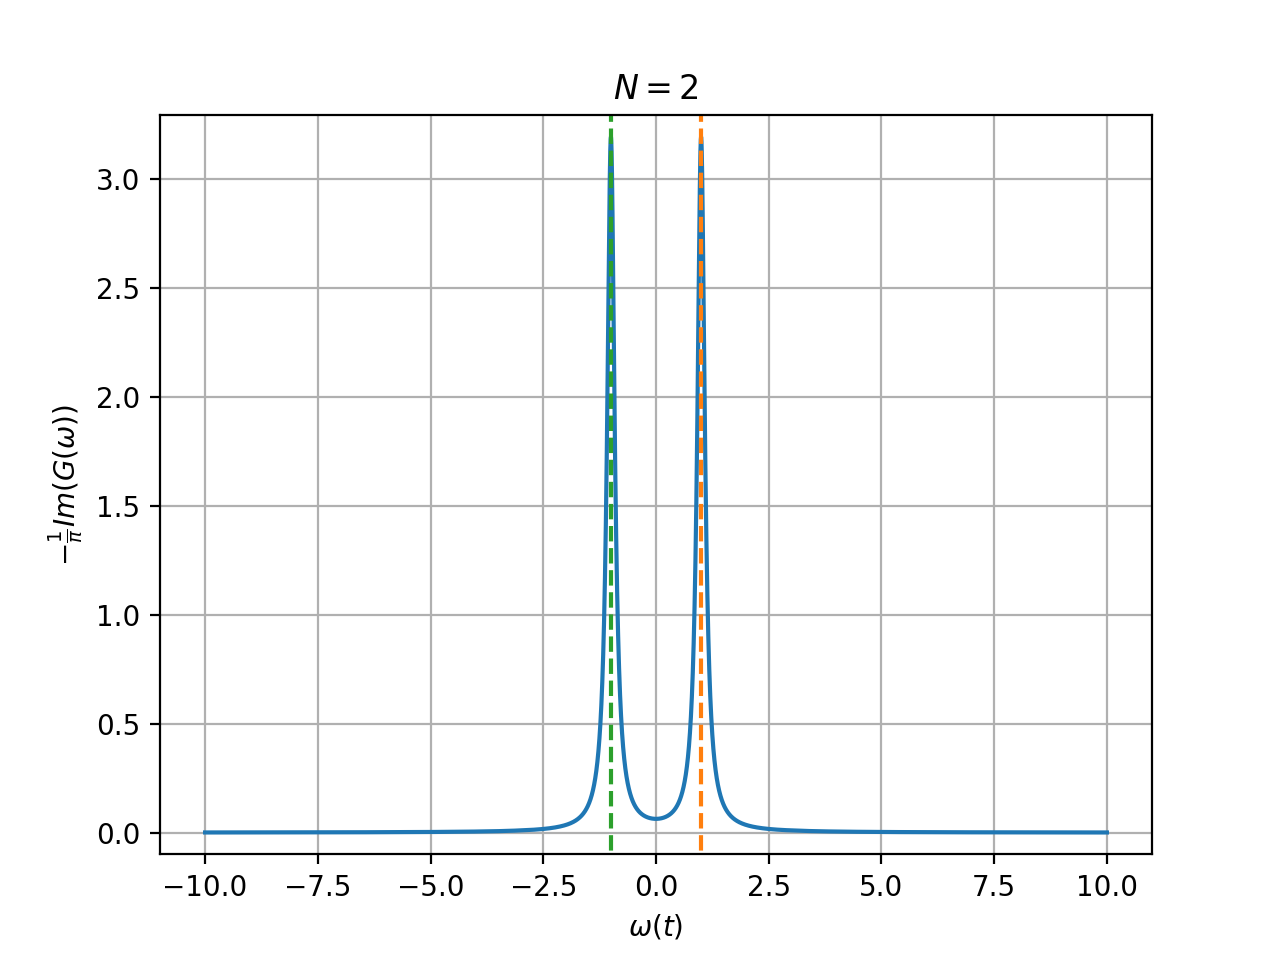
\includegraphics[max width=0.49\linewidth]{lanczosTB2.png}
    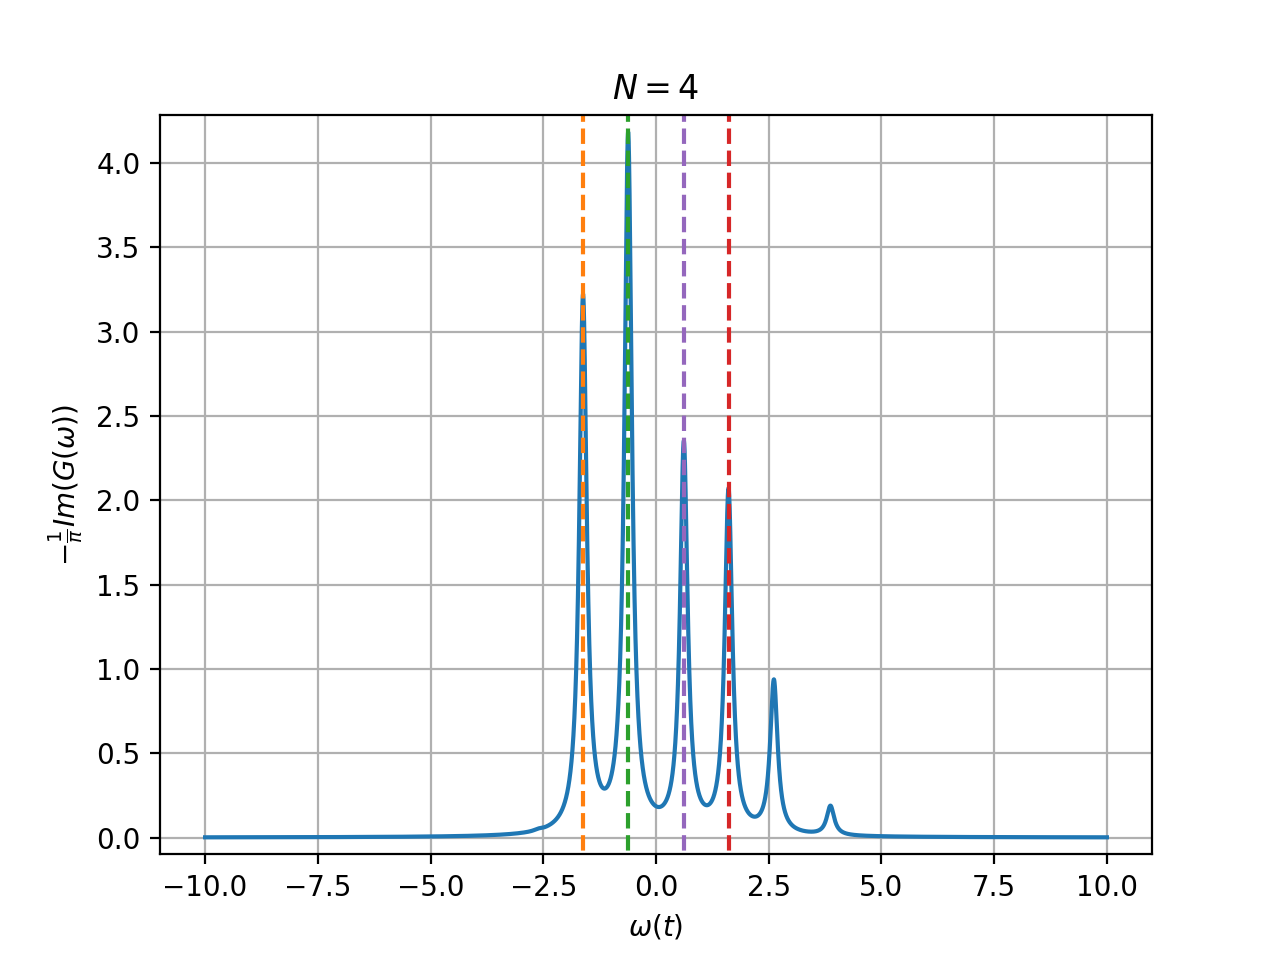
\includegraphics[max width=0.49\linewidth]{lanczosTB4.png}
    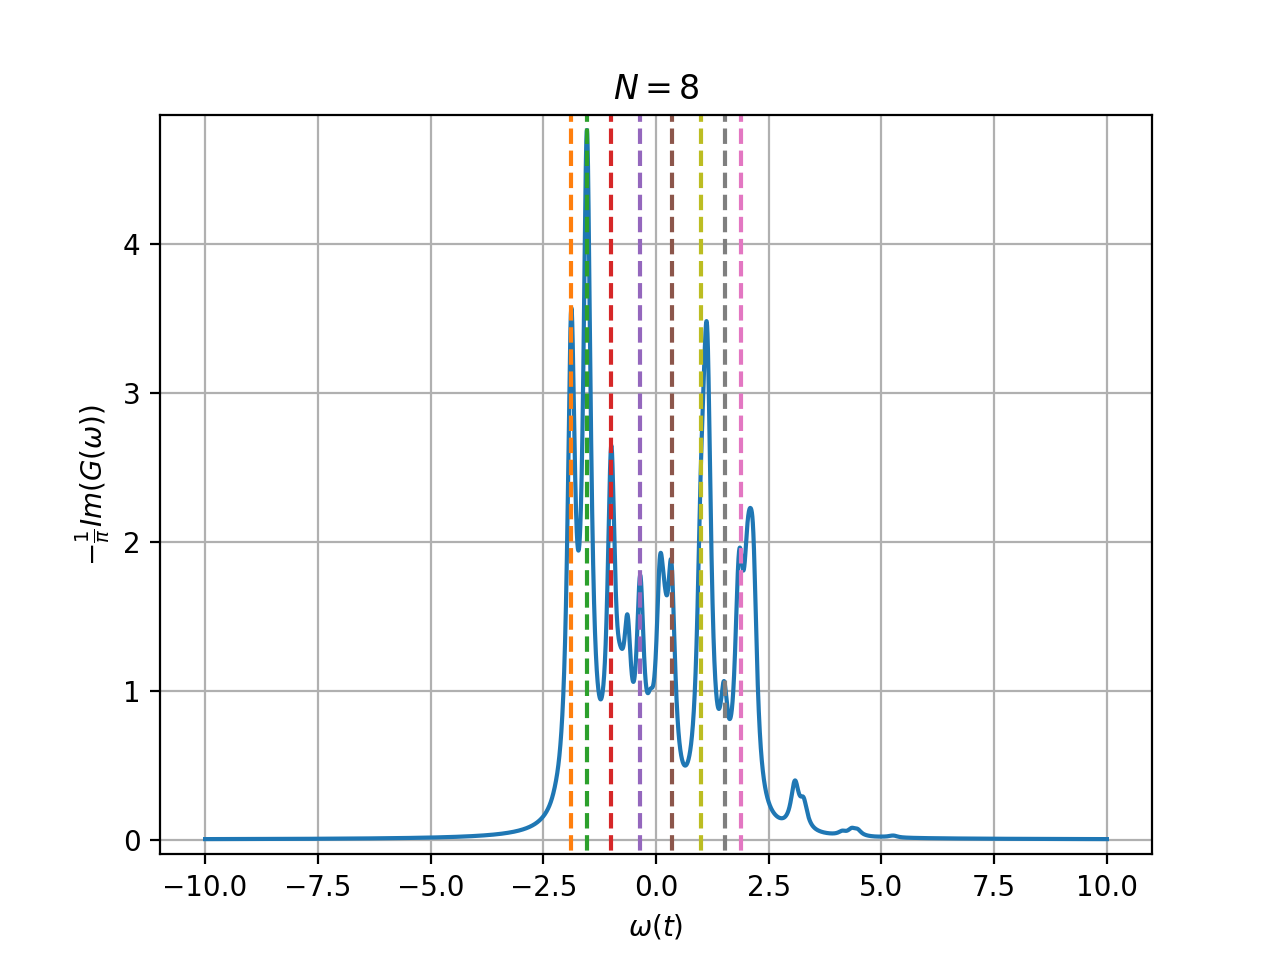
\includegraphics[max width=0.49\linewidth]{lanczosTB8.png}
    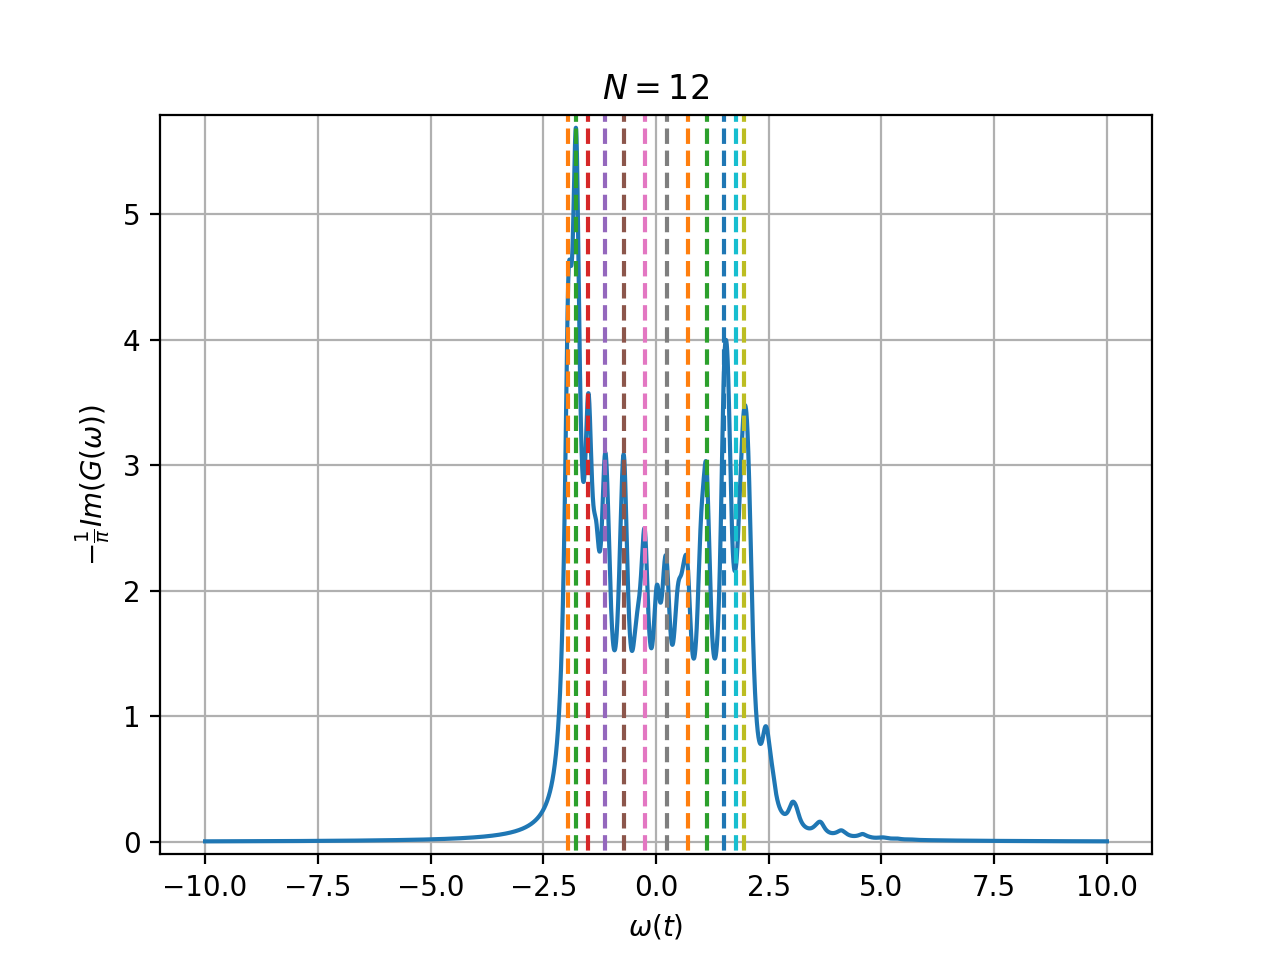
\includegraphics[max width=0.49\linewidth]{lanczosTB12.png}
  \end{center}
  \caption{Densidades de estados calculadas con el algoritmo de Lanczos a partir de la función de Green, para cadenas de tight-binding con condiciones de contorno libres. El valor de $\omega$ está en unidades de $t$, y las lineas punteadas representan los autovalores de la matriz $t_{ij}$, que serían los valores analíticos en los que deberíamos de obtener picos. Los resultados se toman para cadenas de varias longitudes y con 1 electrón para cada spin.}
  \label{fig:greenTB}
\end{figure}

Si observamos la figura \ref{fig:greenTB}, nos podría preocupar que los picos de la densidad de estados no coinciden exactamente, pero vamos a ir viendo que esto es ruido del propio cálculo numérico. Las causas del ruido pueden ser varias:
\begin{itemize}
  \item \textit{Tolerancia limitada}. Aunque estamos exigiendo como criterio de convergencia una tolerancia de $10^{-6}$, el hecho de estar utilizando una diagonalización iterativa y no exacta puede estar causando ruido.
  \item \textit{Las condiciones de contorno no son periódicas}. Tras haber trabajado bastante con el programa, añadir las condiciones periódicas elimina el ruido en gran medida.
  \item \textit{Faltan funciones de Green}. Como ya hemos mencionado, para calcular la función de Green debemos de hacer dos iteraciones más de Lanczos por cada elemento. Esto es muy costoso en tiempo, por lo que, en vez de hacer las iteraciones con la dimensionalidad completa del espacio de Krylov, tomamos sólo un número limitado de raíces de Lanczos para reducir el tiempo de cómputo.
\end{itemize}

Este resultado no es exactamente correcto, excepto en el caso del dímero. Esto se debe a que necesitaríamos, en el caso de $N = 12$, calcular $144$ coeficientes de Lanczos, dos veces, para obtener la función de Green, y el tiempo computacional crece de una manera muy rápida con el número de partículas, como veremos más adelante. Es por ello que nos restringimos a calcular unos pocos coeficientes, y vemos que la densidad de estados está más o menos convergida, sin llegar a ser la solución exacta.

Otra señal de buen funcionamiento es que en la figura \ref{fig:greenTB}, vemos como al ir aumentando el número de partículas, la densidad de estados va tendiendo a la que obtuvimos analíticamente en el apartado de resolución analítica del modelo tight-binding. Se observa la formación de dos picos muy prominentes en los lados, debido a las singularidades de Van-Hove, y la forma parabólica en el centro que es parecida a la que veíamos en la otra figura.
\subsubsection{El dímero de Hubbard}

El modelo de Hubbard tiene soluciones unidimensionales analíticas. En esta sección nos vamos a centrar en la dada para el dímero, osea, el caso de dos partículas. La solución analítica se puede encontrar en la referencia \cite{mironov2025dimerhubbardmodelexact}. Vamos a comparar la densidad de estados que calculamos con el algoritmo de Lanczos con la calculada en la referencia.
\begin{figure}[h!]
  \begin{center}
    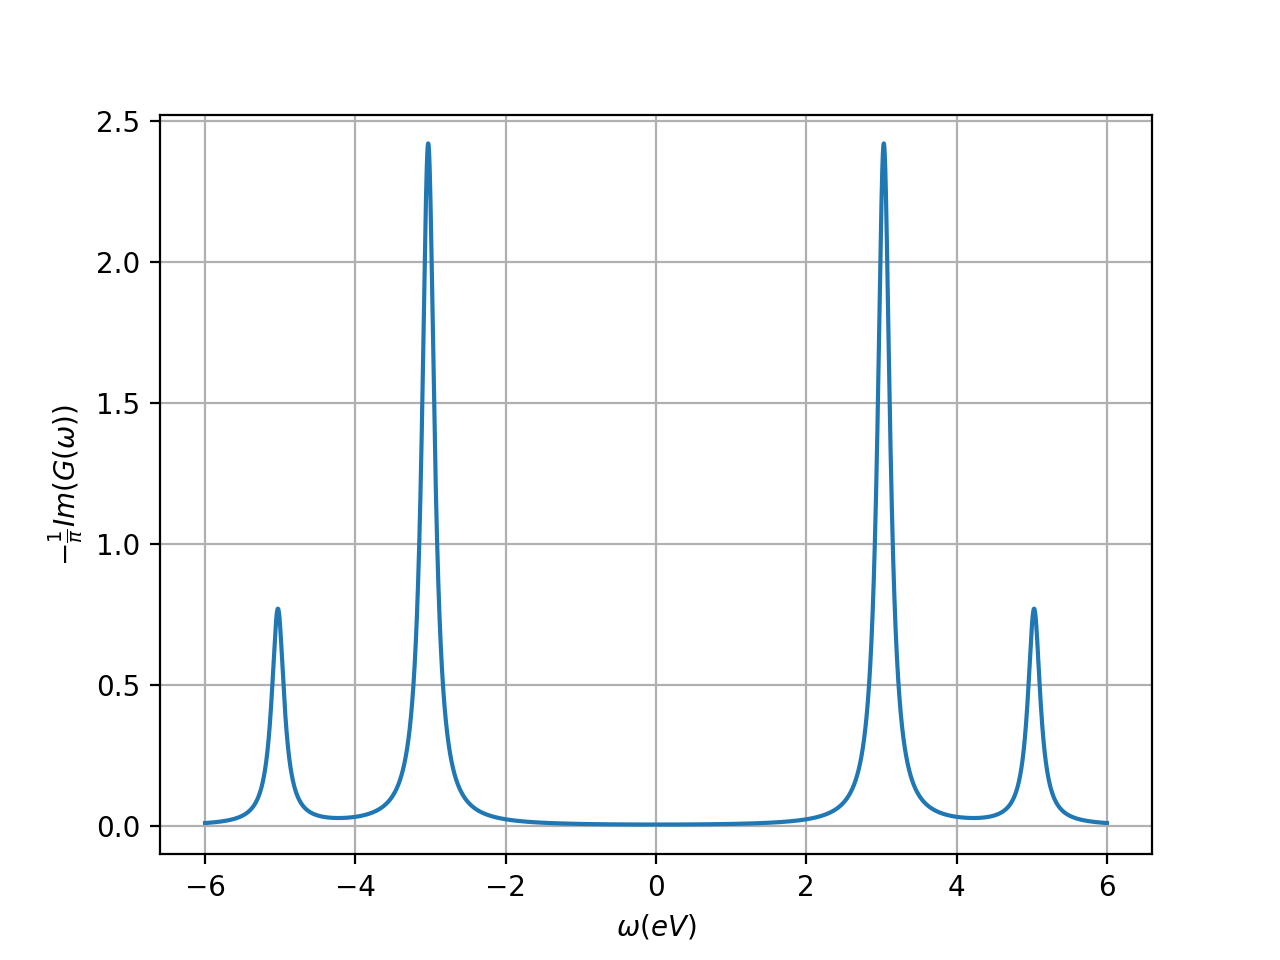
\includegraphics[max width=\linewidth]{lanczosHubbard2.png}
  \end{center}
  \caption{Densidad de estados obtenida con el algoritmo de Lanczos. Aquí se toma $\varepsilon_0 = -3.5 eV$, $U = 7 eV$ y $t = -1 eV$. El valor de $\eta = 0.1$.}
  \label{fig:lancvref}
\end{figure}

Como podemos observar en la figura \ref{fig:lancvref}, la posición de los picos coincide entre los dos programas. En este caso, vemos como al añadir la interacción se van formando unos picos secundarios. Más adelante, observaremos que estos picos secundarios van creciendo según hacemos más fuerte la interacción.

También podemos comparar con las densidades de estados de la referencia \cite{GreeneDiniz2024}, donde utilizan computación cuántica para calcular varias funciones de Green en cadenas. Podemos ver, por ejemplo, el caso de cuatro núcleos. Se puede observar en la figura \ref{fig:quantumLanczosHubbard}
\begin{figure}[h!]
  \begin{center}
    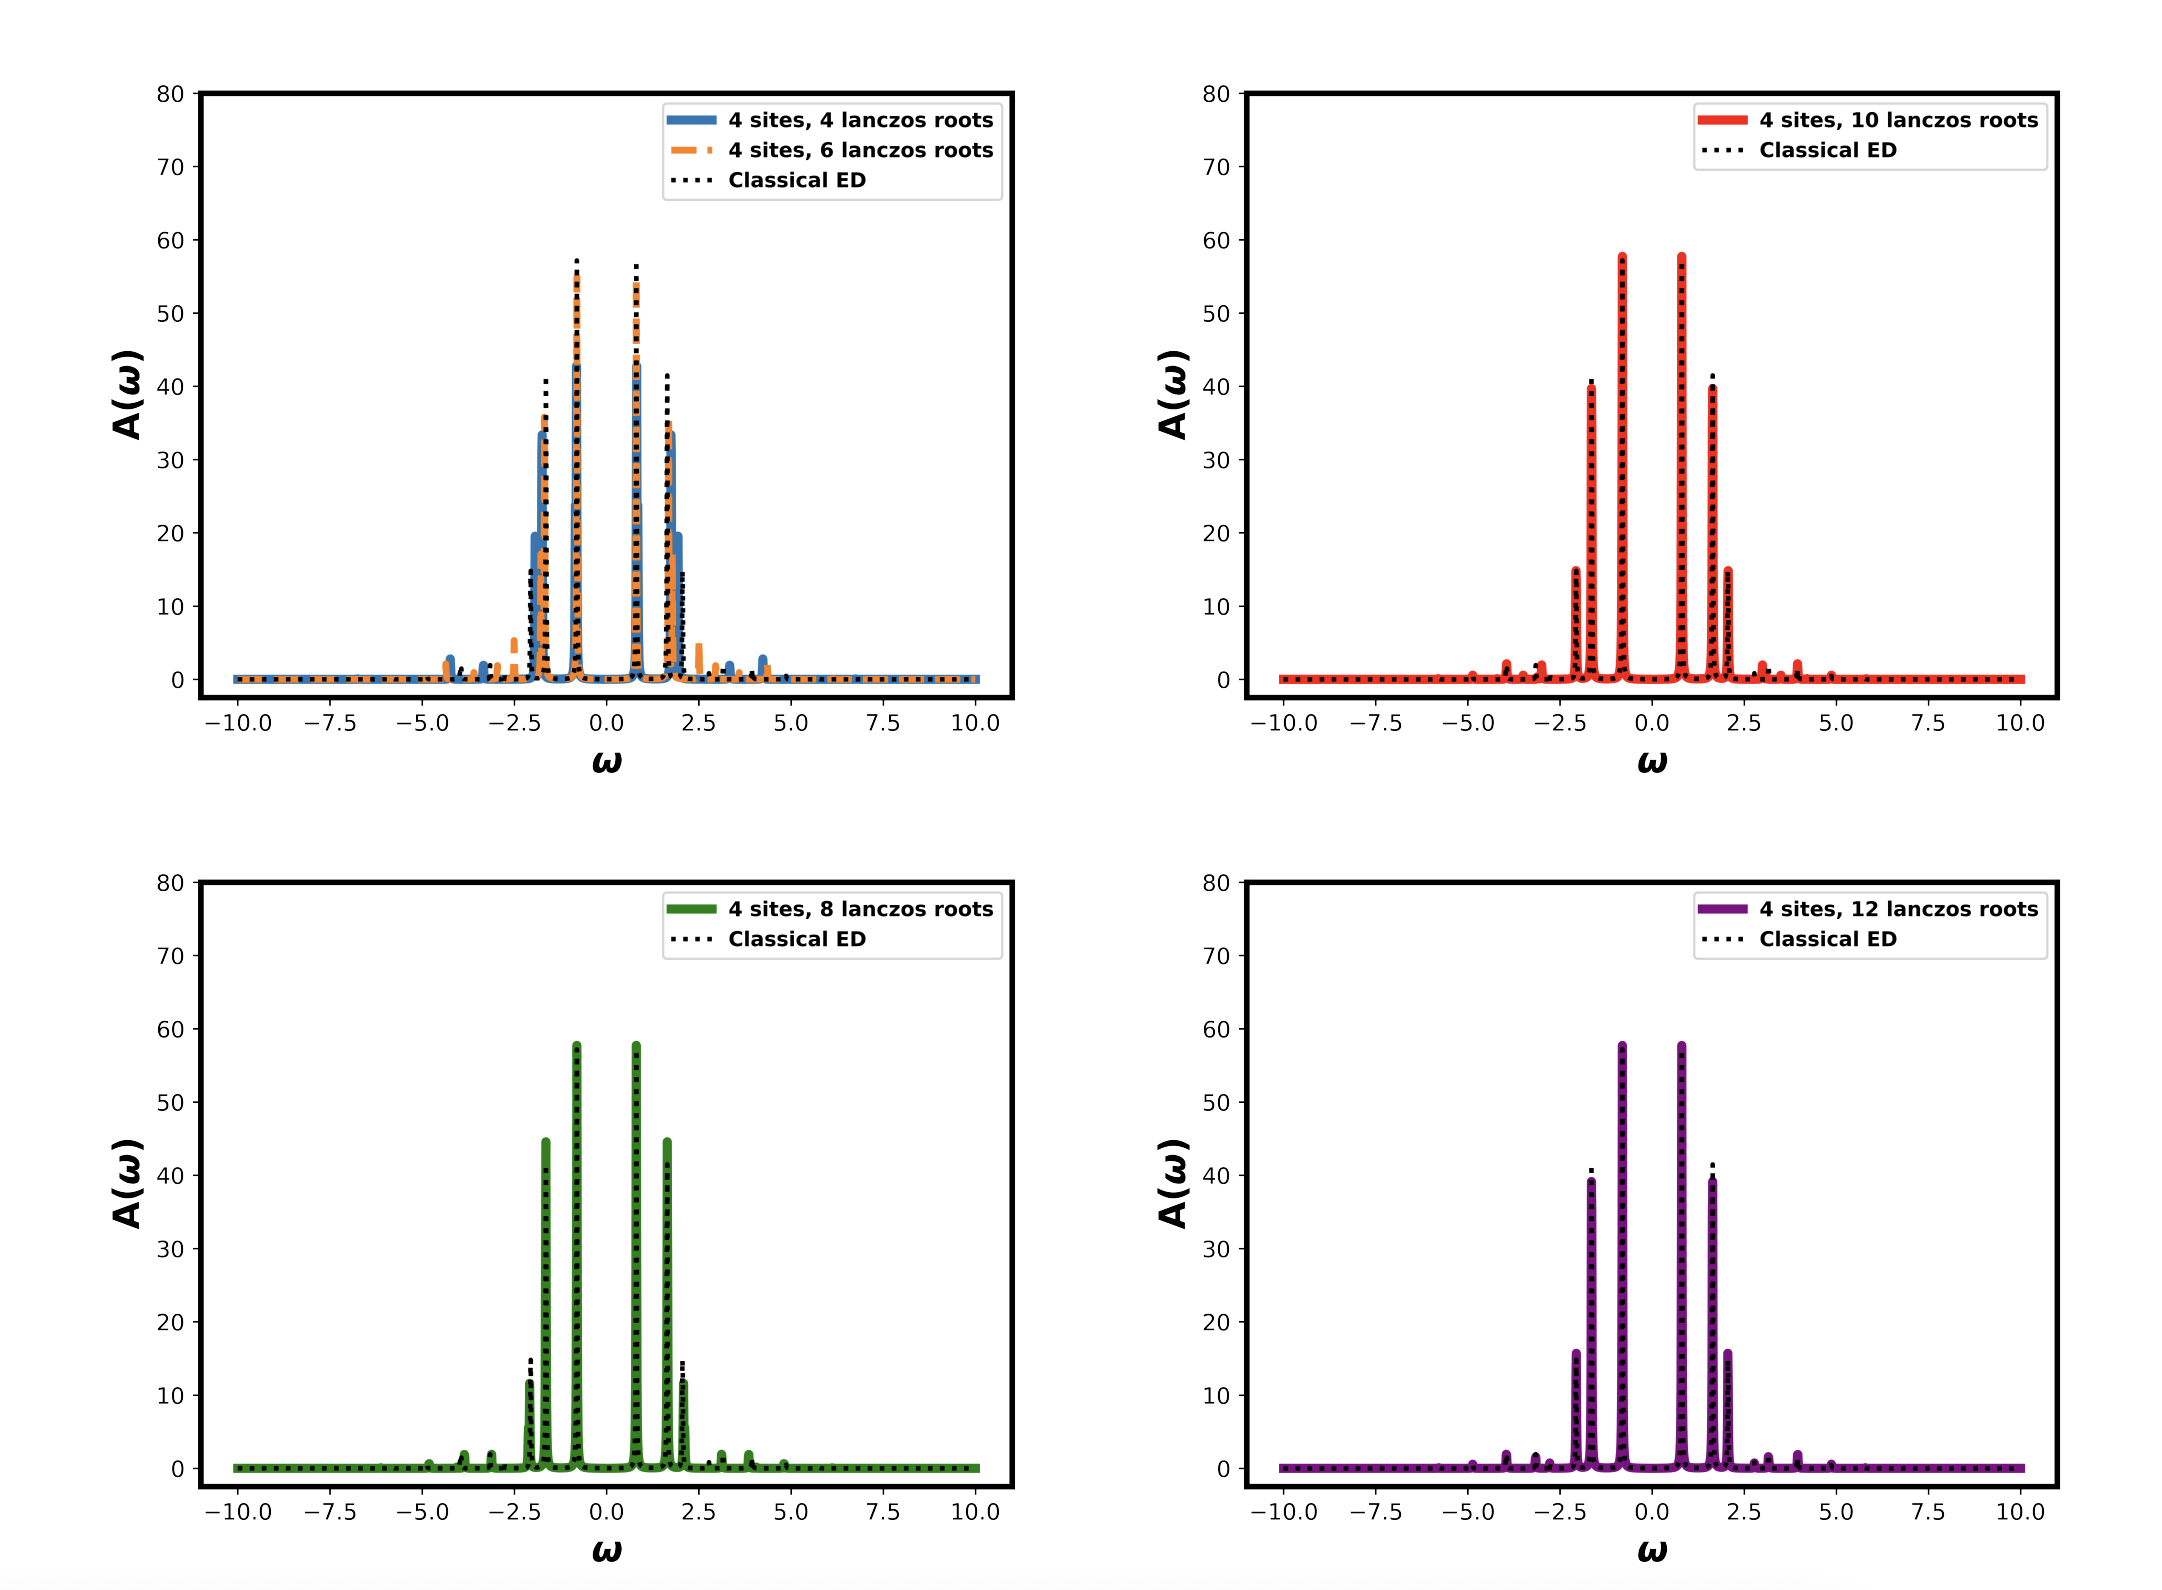
\includegraphics[max width=\linewidth]{quantumComputed.png}
  \end{center}
  \caption{Figura obtenida de la referencia \cite{GreeneDiniz2024}, en el que se calcula, para el caso en que $\left|\frac{U}{t}\right| = 2$, la parte imaginaria de la función de Green. Los autores originales realizan el estudio variando el número de raíces de Lanczos.}
  \label{fig:quantumLanczosHubbard}
\end{figure}

Los autores de la figura \ref{fig:quantumLanczosHubbard} han realizado el desarrollo para la cadena semillena, es por ello que haremos lo mismo. Los resultados obtenidos con nuestro programa se pueden ver en \ref{fig:lanczosHubbard4}.
\begin{figure}[h!]
  \begin{center}
    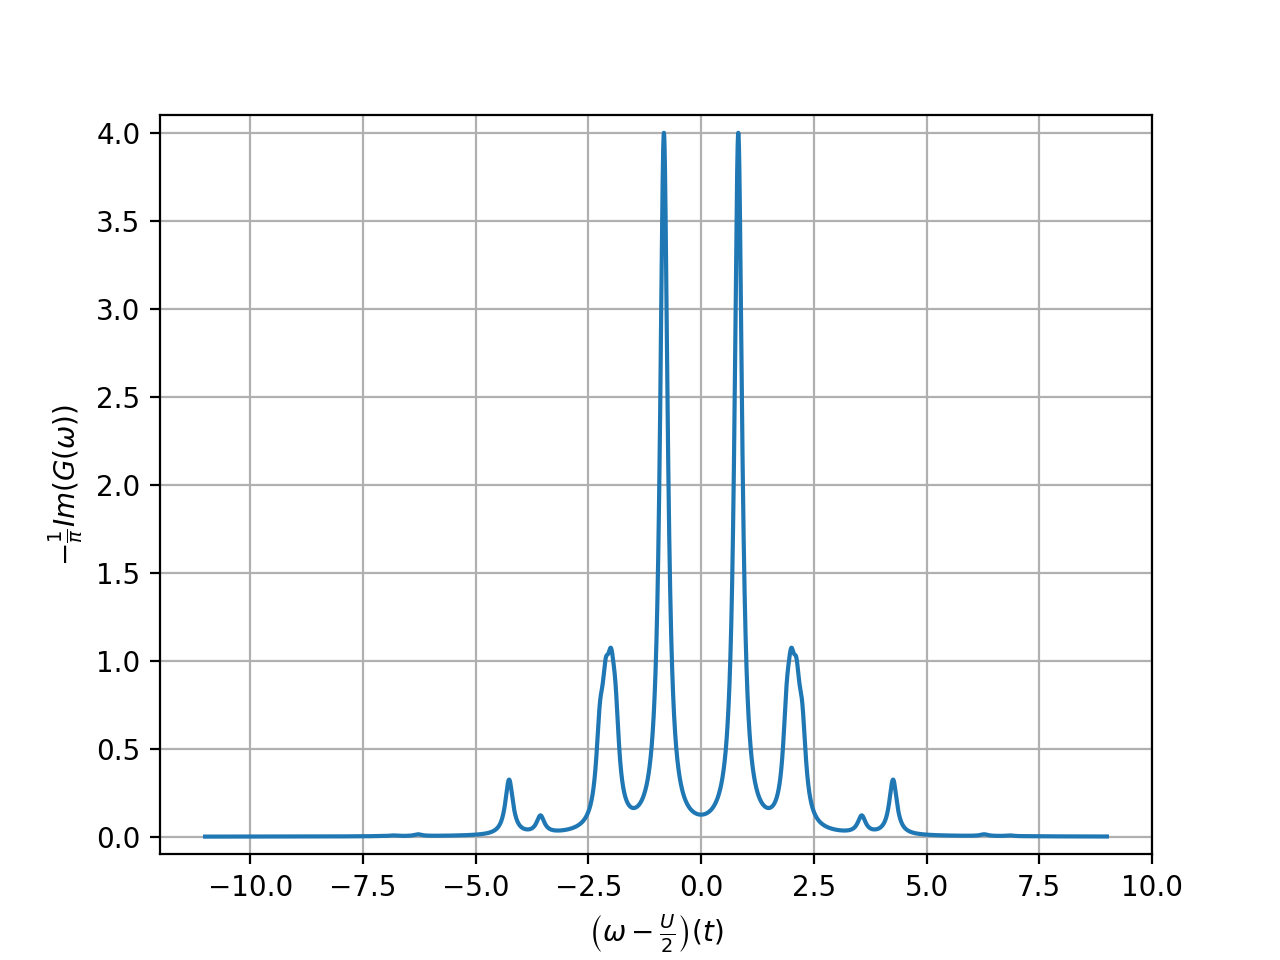
\includegraphics[max width=\linewidth]{lanczosHubbard4weak.png}
  \end{center}
  \caption{Densidad de estados obtenida para el caso $\left|\frac{U}{t}\right| = 2$. El valor de $\omega$ está en unidades de $t$. Nos encontramos en un caso con cuatro núcleos en la cadena y condiciones de contorno libres.}
  \label{fig:lanczosHubbard4}
\end{figure}

Para el modelo de Hubbard con los mismos parámetros que los autores de \cite{GreeneDiniz2024}, obtenemos que las funciones se parecen lo suficiente, sobre todo en la distribución de los picos, que es lo que nos interesa.

Cabe destacar que ahora centramos los picos en $U/2$. A lo largo del trabajo, observaremos este desplazamiento del cero, que será una de las características esenciales del modelo.
\subsection{Cálculos en la cadena de Hubbard}
\subsubsection{Transición metal-aislante}

Vamos a utilizar valores de $\varepsilon_0 = 0$ y $U, t > 0$. Volvamos al caso del dímero. Vamos a representar las funciones de Green para distintos valores de $\left|\frac{U}{t}\right|$, de este modo, vamos a ver el efecto de aumentar el término de interacción.
\begin{figure}[h!]
  \begin{center}
    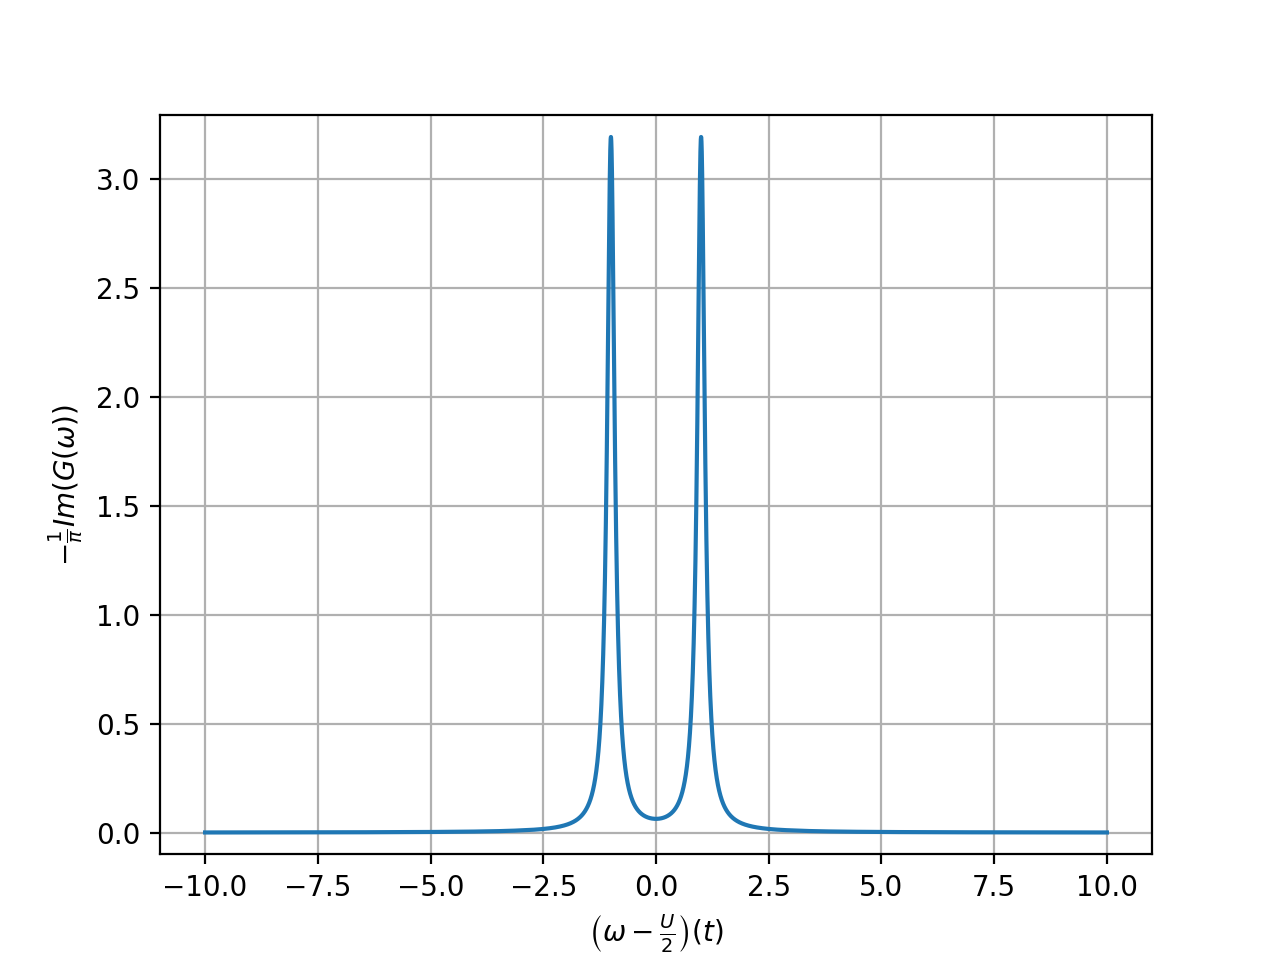
\includegraphics[max width=0.49\linewidth]{lanczosHubbard2U0Imag.png}
    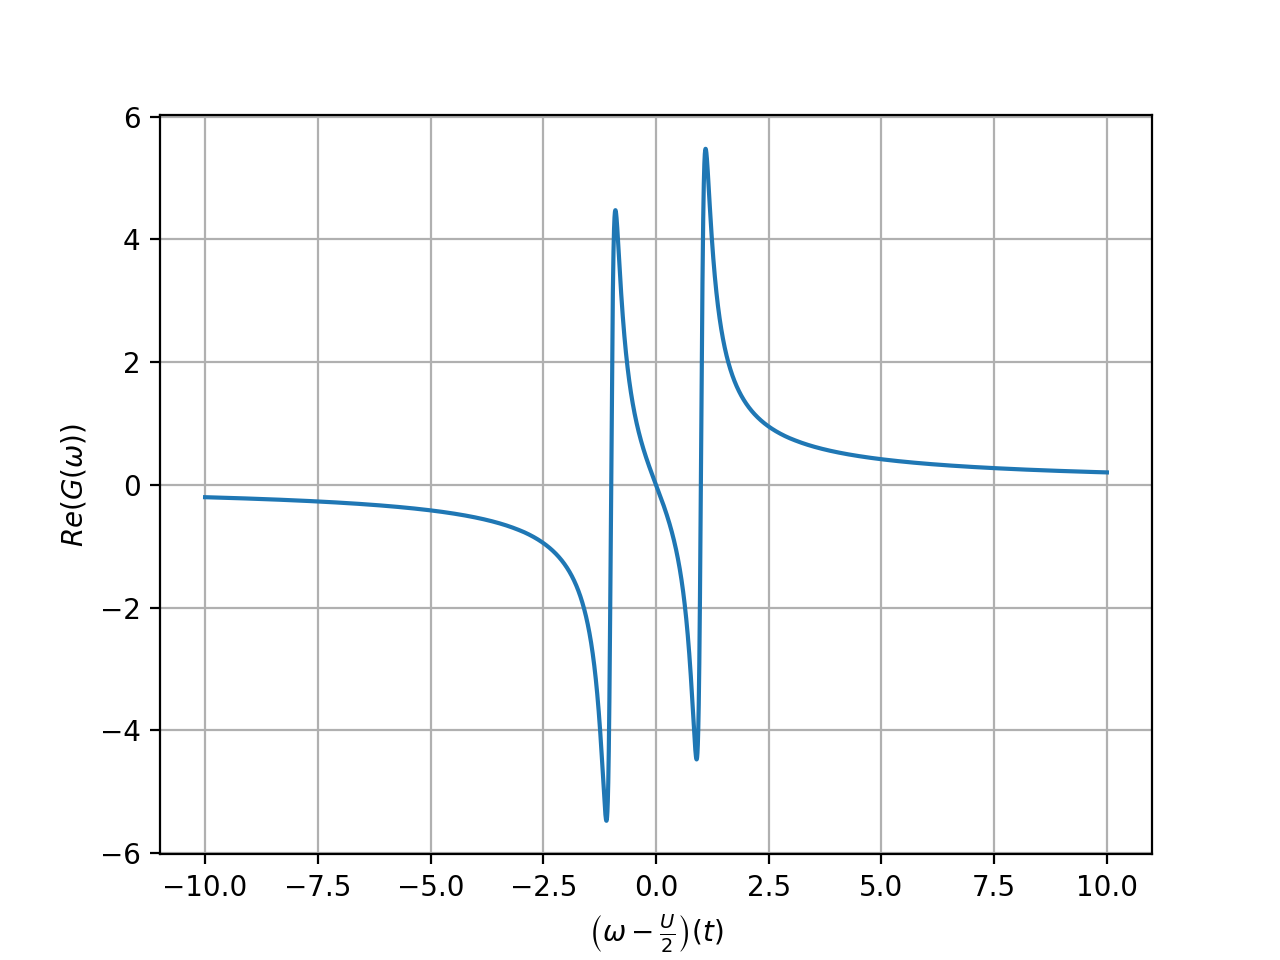
\includegraphics[max width=0.49\linewidth]{lanczosHubbard2U0Real.png}
    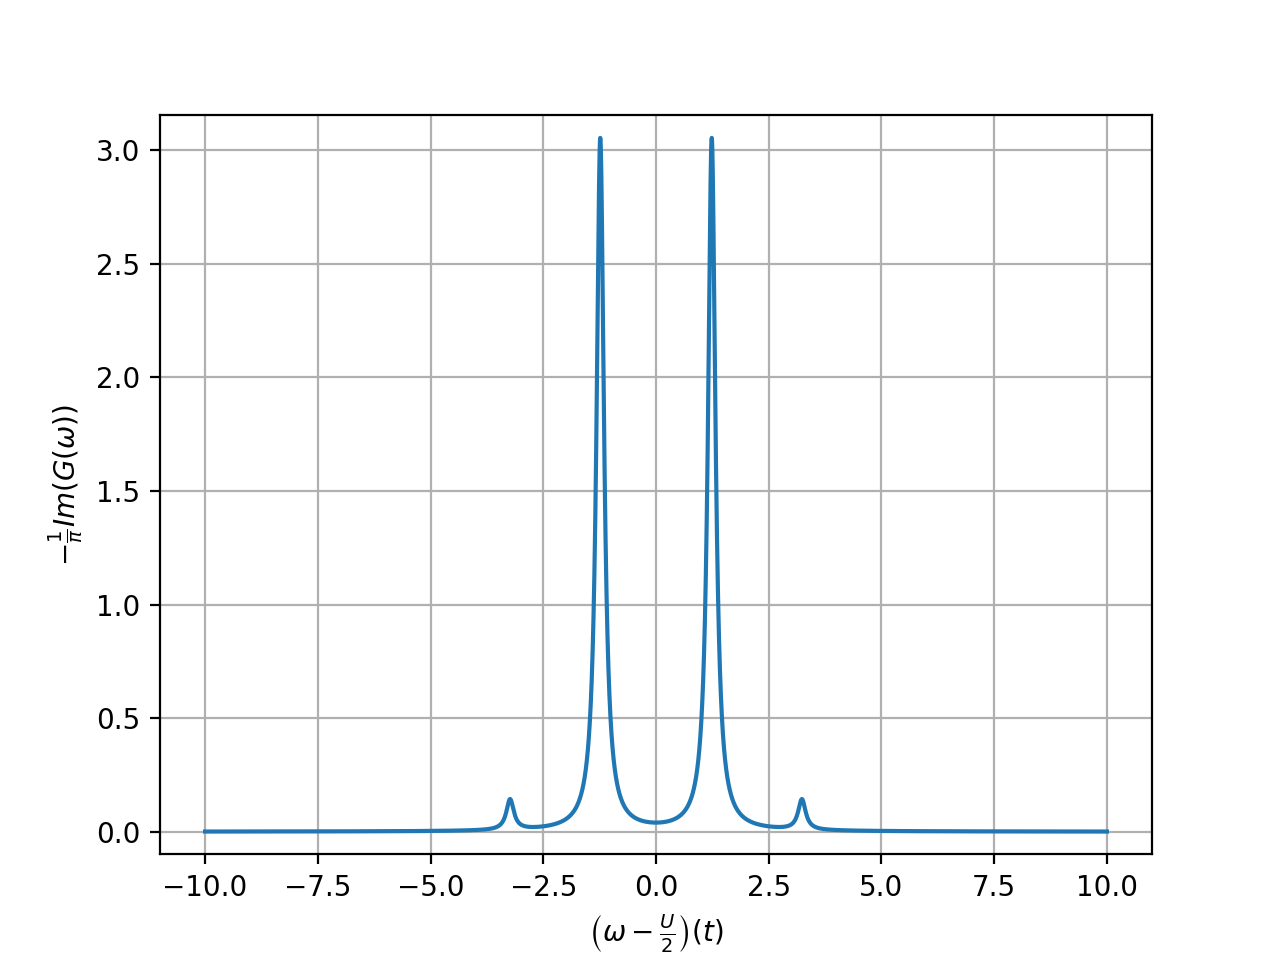
\includegraphics[max width=0.49\linewidth]{lanczosHubbard2U2Imag.png}
    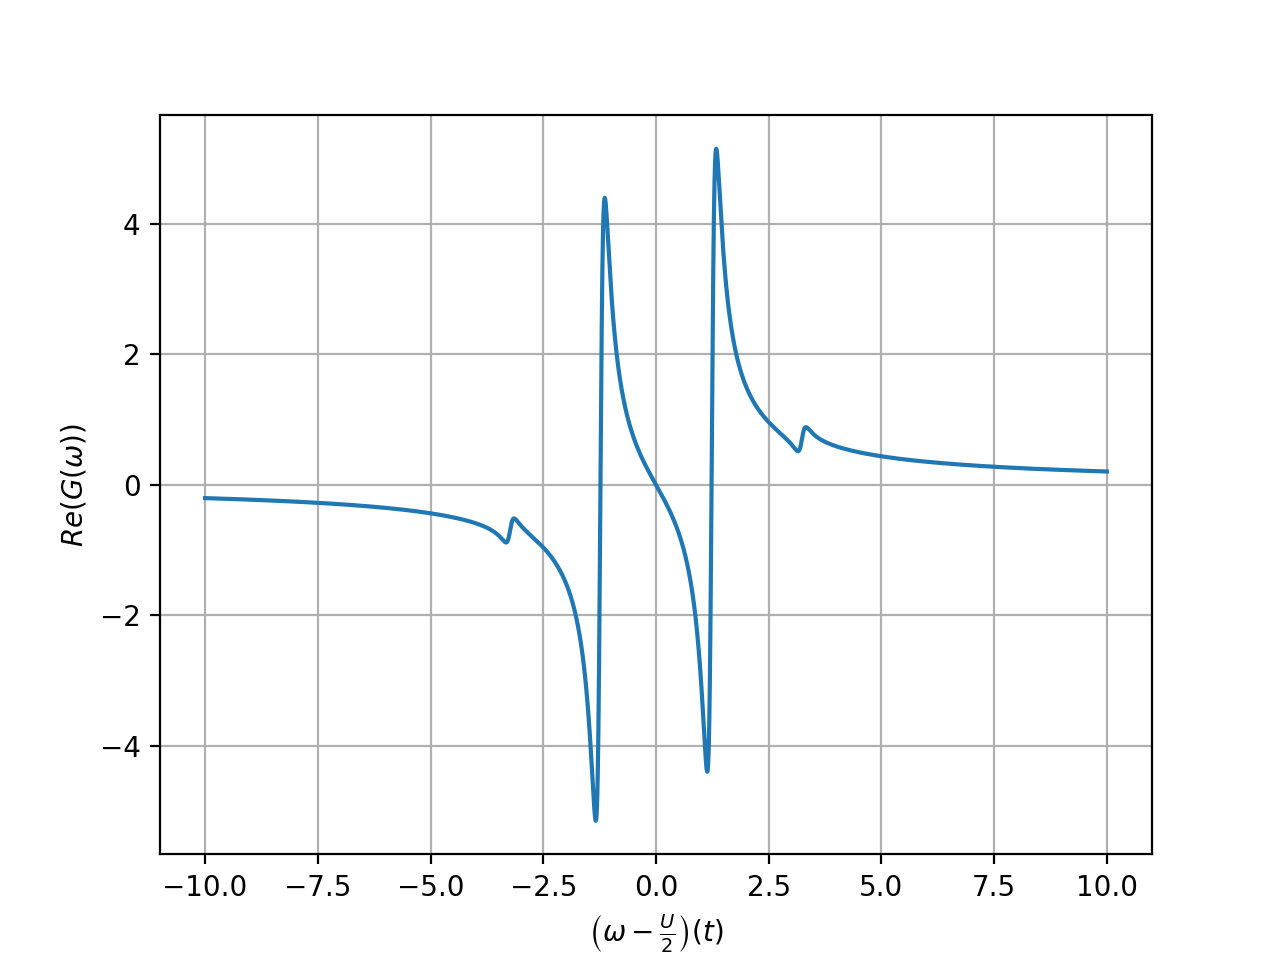
\includegraphics[max width=0.49\linewidth]{lanczosHubbard2U2Real.png}
    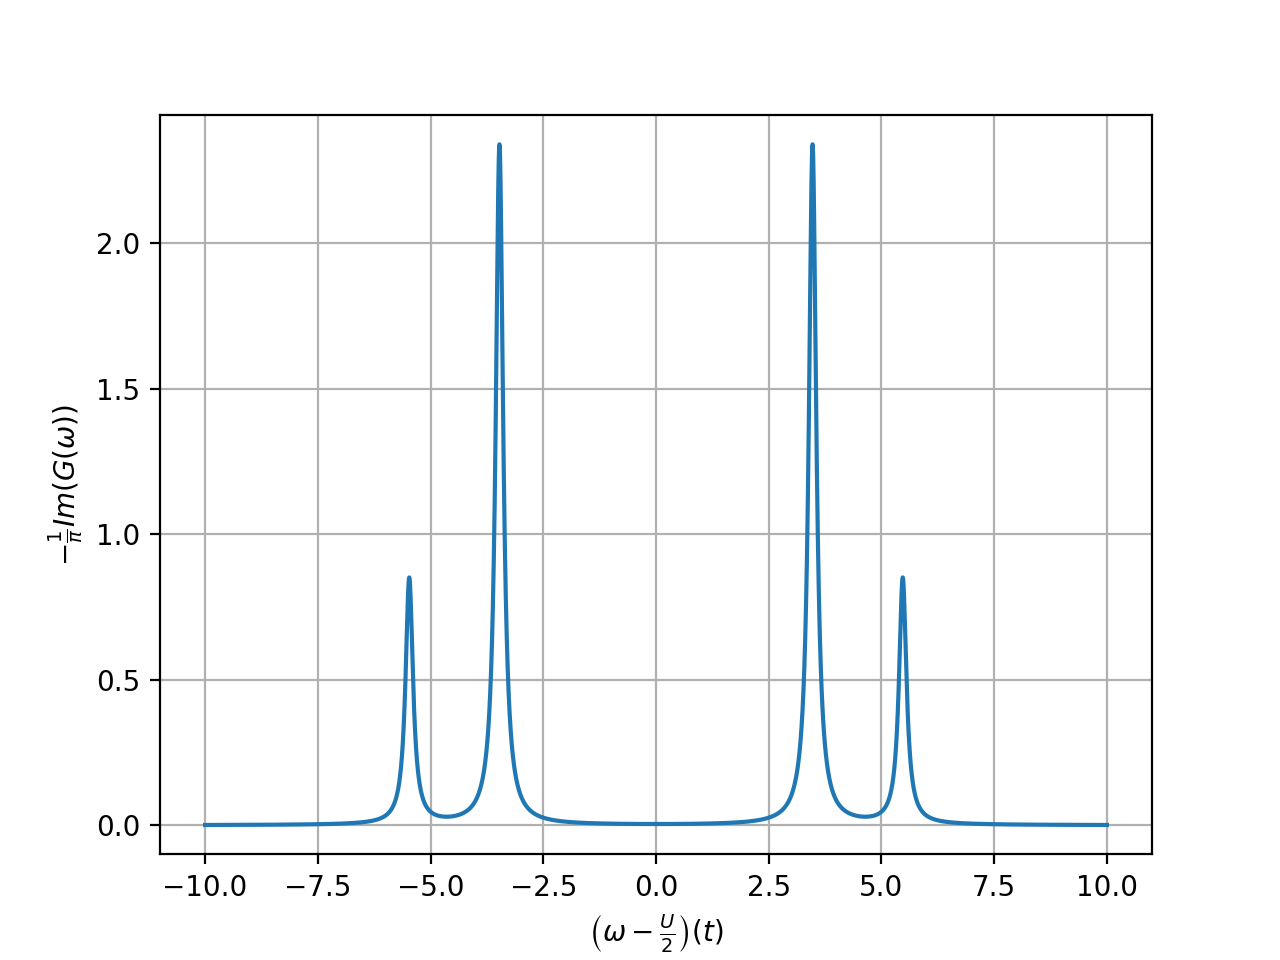
\includegraphics[max width=0.49\linewidth]{lanczosHubbard2U8Imag.png}
    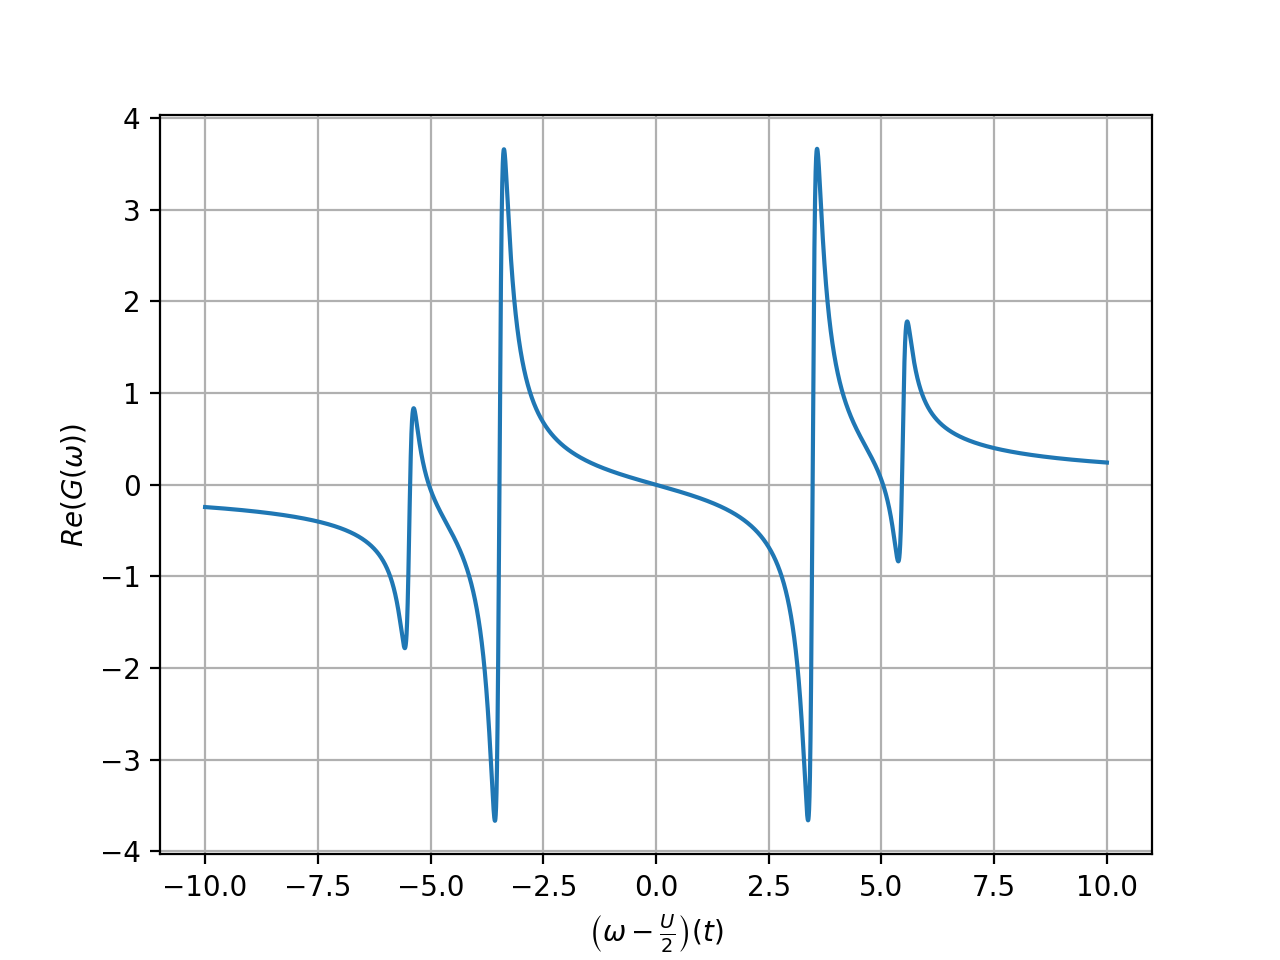
\includegraphics[max width=0.49\linewidth]{lanczosHubbard2U8Real.png}
  \end{center}
  \caption{Partes imaginaria y real de la función de Green, calculadas, según orden de aparición, para $U = 0t$, $U = 2t$ y $U = 8t$. Se puede comprobar que las posiciones de los picos y las alturas coinciden con la referencia \cite{GreeneDiniz2024}.}
  \label{fig:hubbardTransition}
\end{figure}

Fijémonos en las primeras figuras de \ref{fig:hubbardTransition}. En nuestro caso, la energía de Fermi se va a ubicar siempre en cero, es decir, siempre centraremos el sistema en la energía de Fermi. Esto se puede comprobar muy fácilmente viendo que, la parte llena de partículas de la densidad de estados es justamente la de la izquierda, comprobemos que se cumple para este caso, observese la figura \ref{fig:greenFilled}.
\begin{figure}[h!]
  \begin{center}
    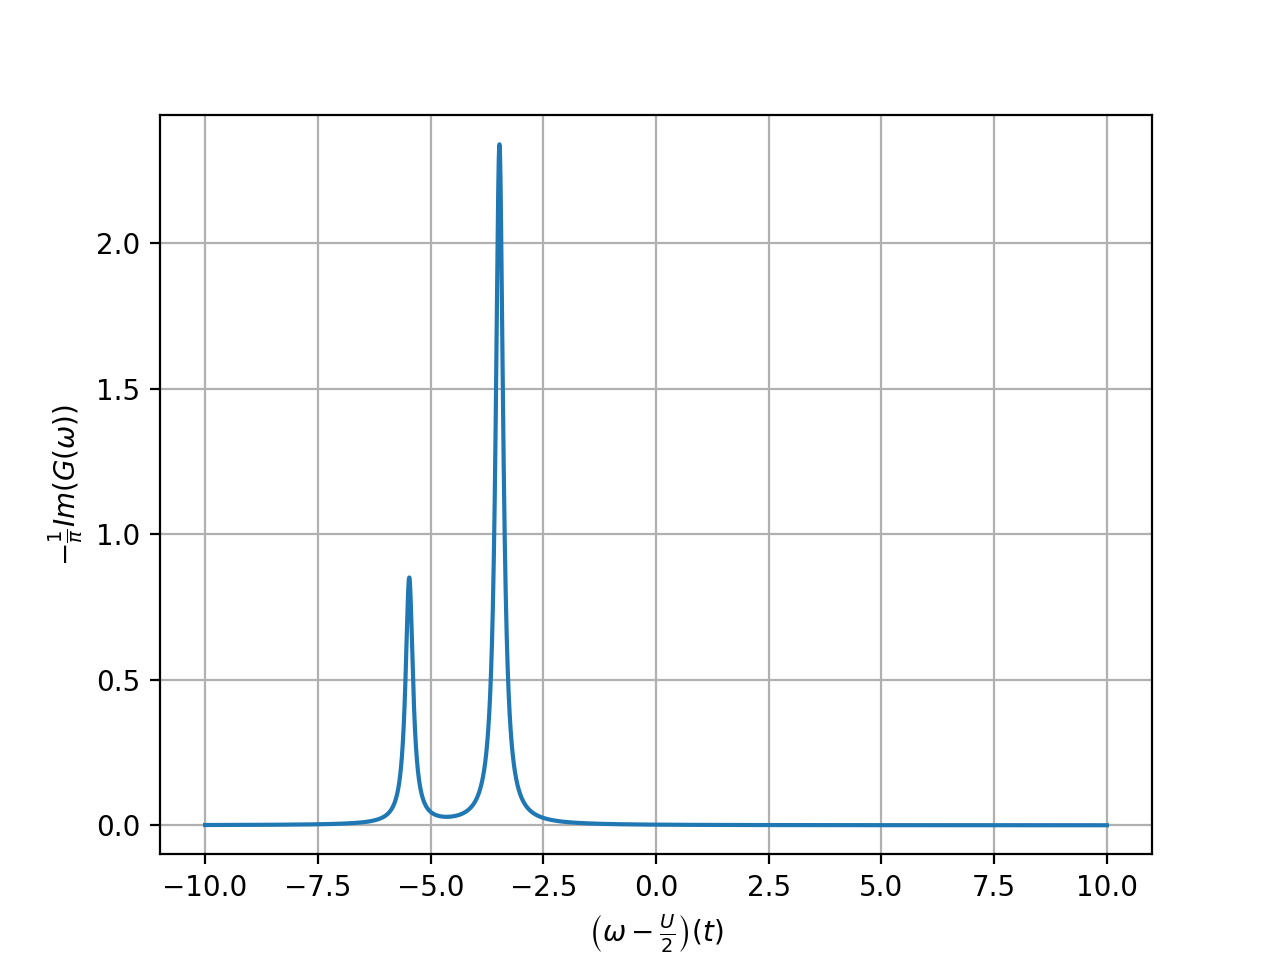
\includegraphics[max width=0.49\linewidth]{lanczosHubbard2U8ImagFilled.png}
    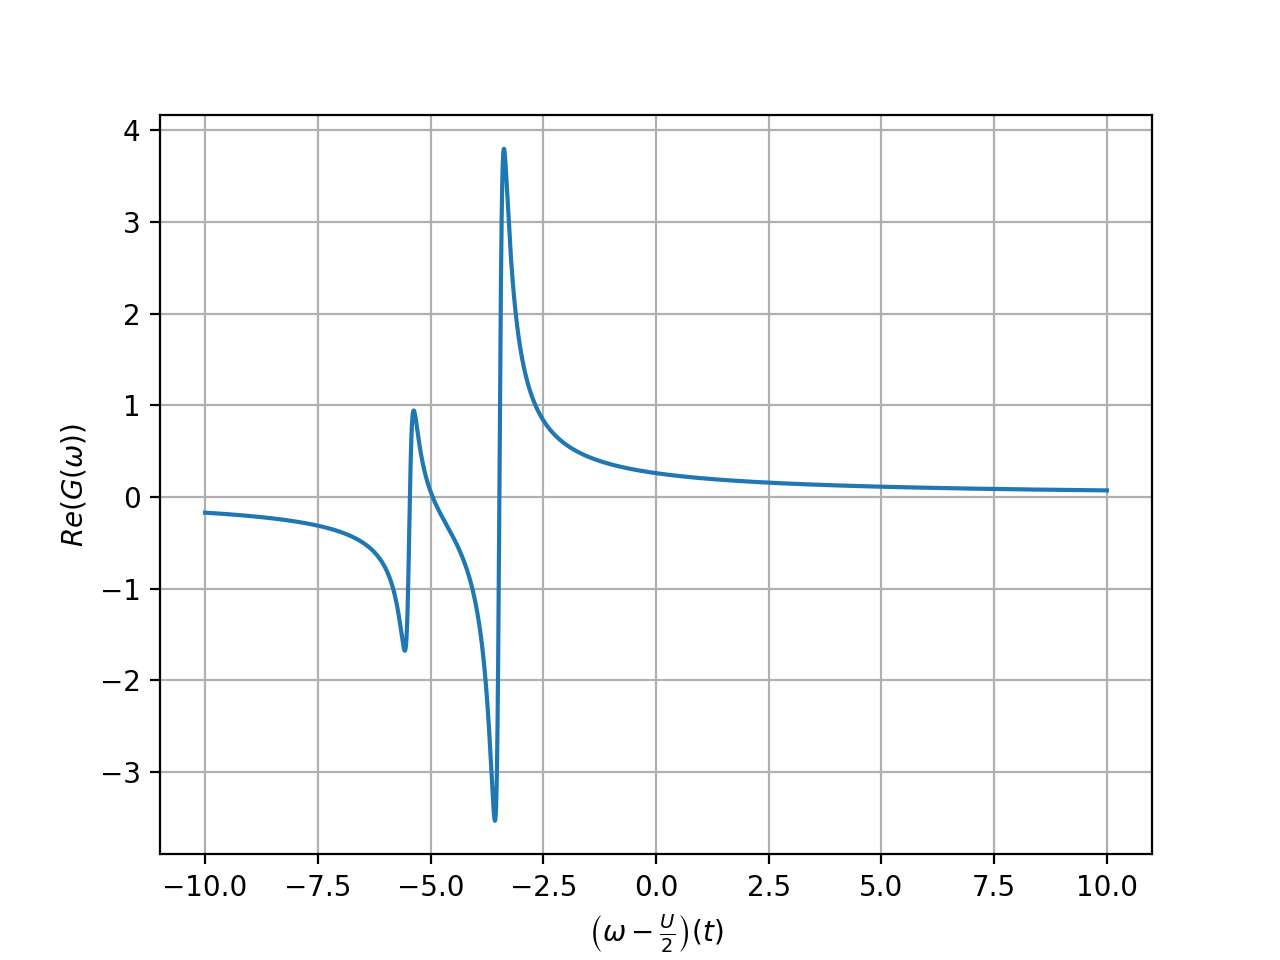
\includegraphics[max width=0.49\linewidth]{lanczosHubbard2U8RealFilled.png}
  \end{center}
  \caption{Densidad de estados asociada a la parte de partículas, $c_i^{\dagger}c_i$, de la función de Green, calculada para el dímero de Hubbard con $U = 8t$.}
  \label{fig:greenFilled}
\end{figure}

En este caso, el nivel inferior está lleno. Sin embargo, puesto que el parámetro de hopping depende inversamente con la distancia, uno puede imaginar que al añadir muchos átomos a la cadena, esta densidad de estados va a tender a la de la cadena infinita, y los átomos van a estar muy juntos. En este caso, tendremos una densidad sin gaps, como vimos en la figura \ref{fig:dosTB}. Aquí el material se comportaría como un metal.

Volvamos a observar qué sucede en la figura \ref{fig:hubbardTransition} al aumentar $U$. Observamos que el aumento de $U$ va generando dos bandas definidas, separadas por un gap muy grande, debido al término de interacción. Podemos volver al caso de 6 partículas para ver cómo se van separando las bandas según vamos aumentando el término de interacción. Esto se puede observar en la figura \ref{fig:hubbardTransition6}.
\begin{figure}[h!]
  \begin{center}
    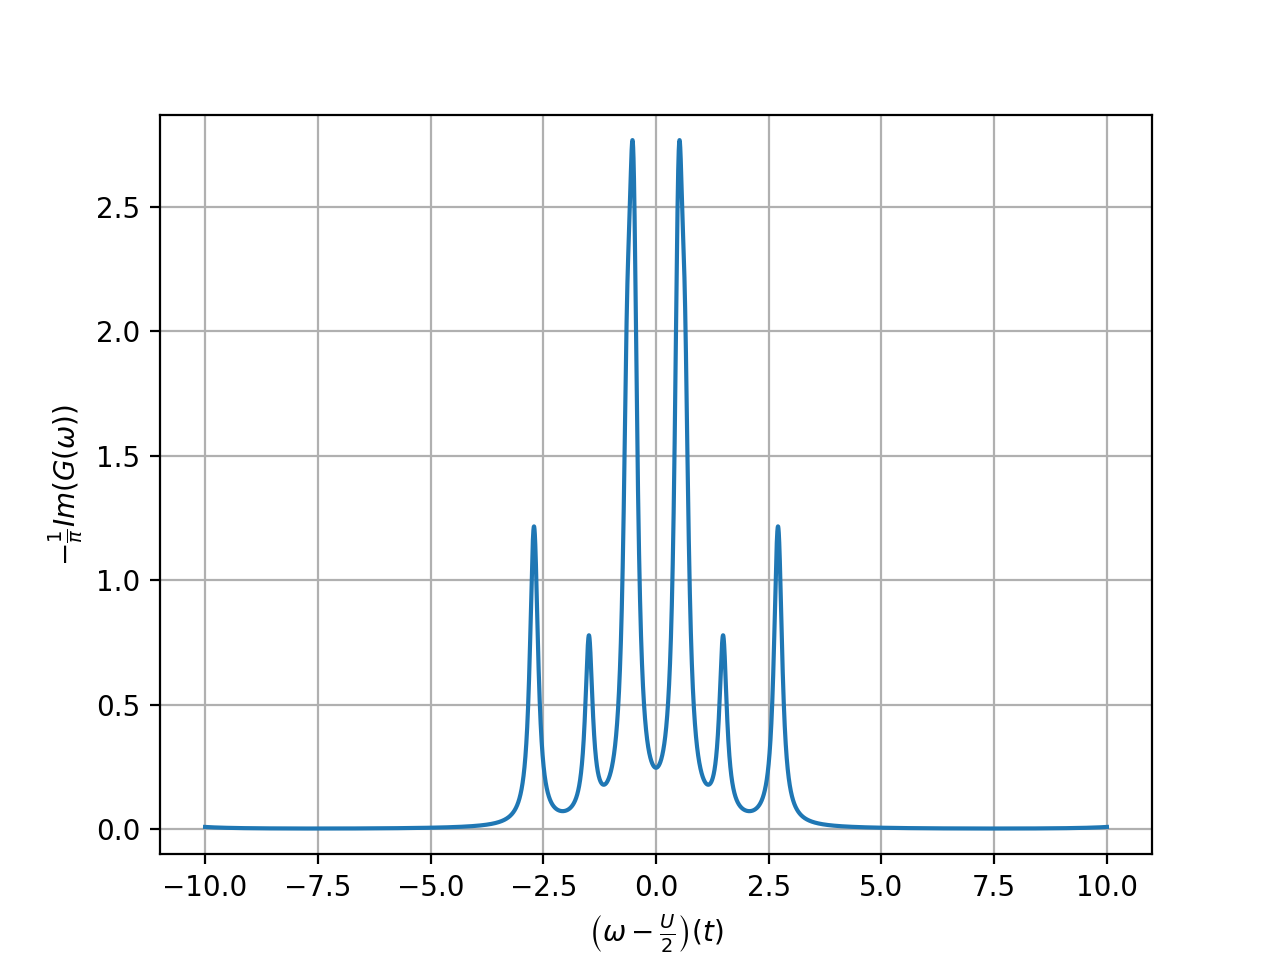
\includegraphics[max width=0.49\linewidth]{lanczosHubbard6U0Imag.png}
    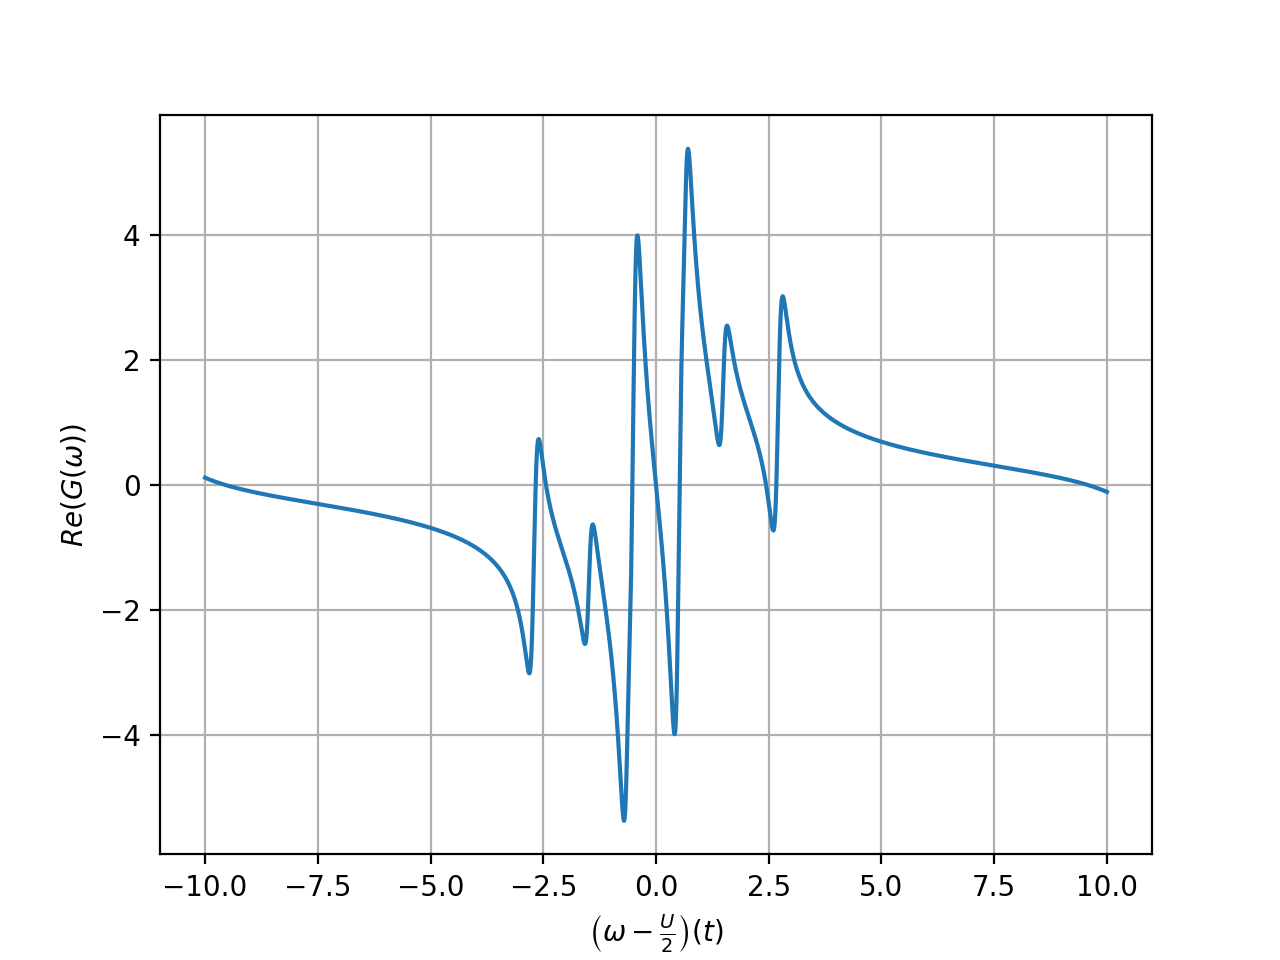
\includegraphics[max width=0.49\linewidth]{lanczosHubbard6U0Real.png}
    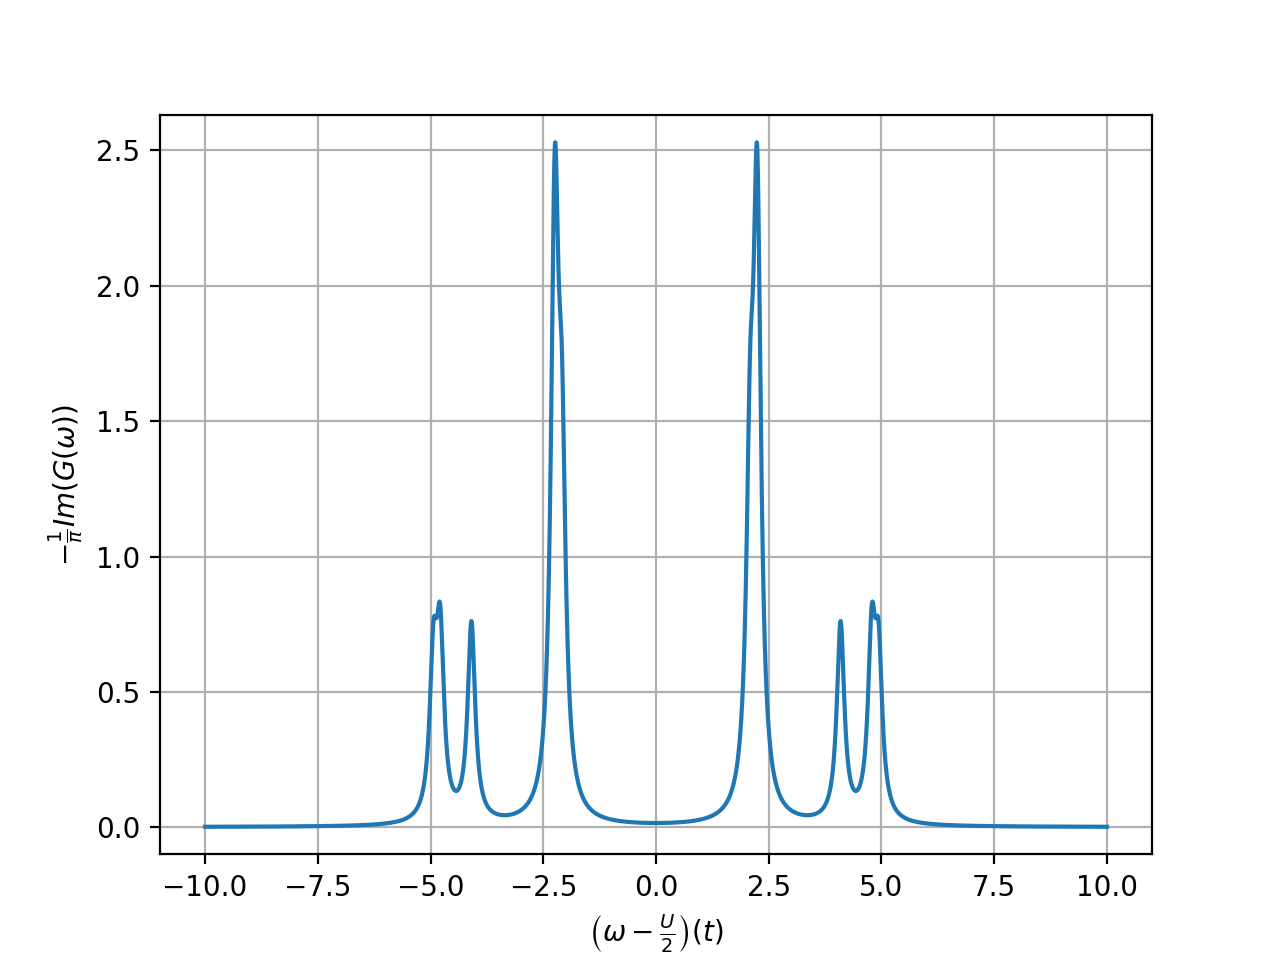
\includegraphics[max width=0.49\linewidth]{lanczosHubbard6U6Imag.png}
    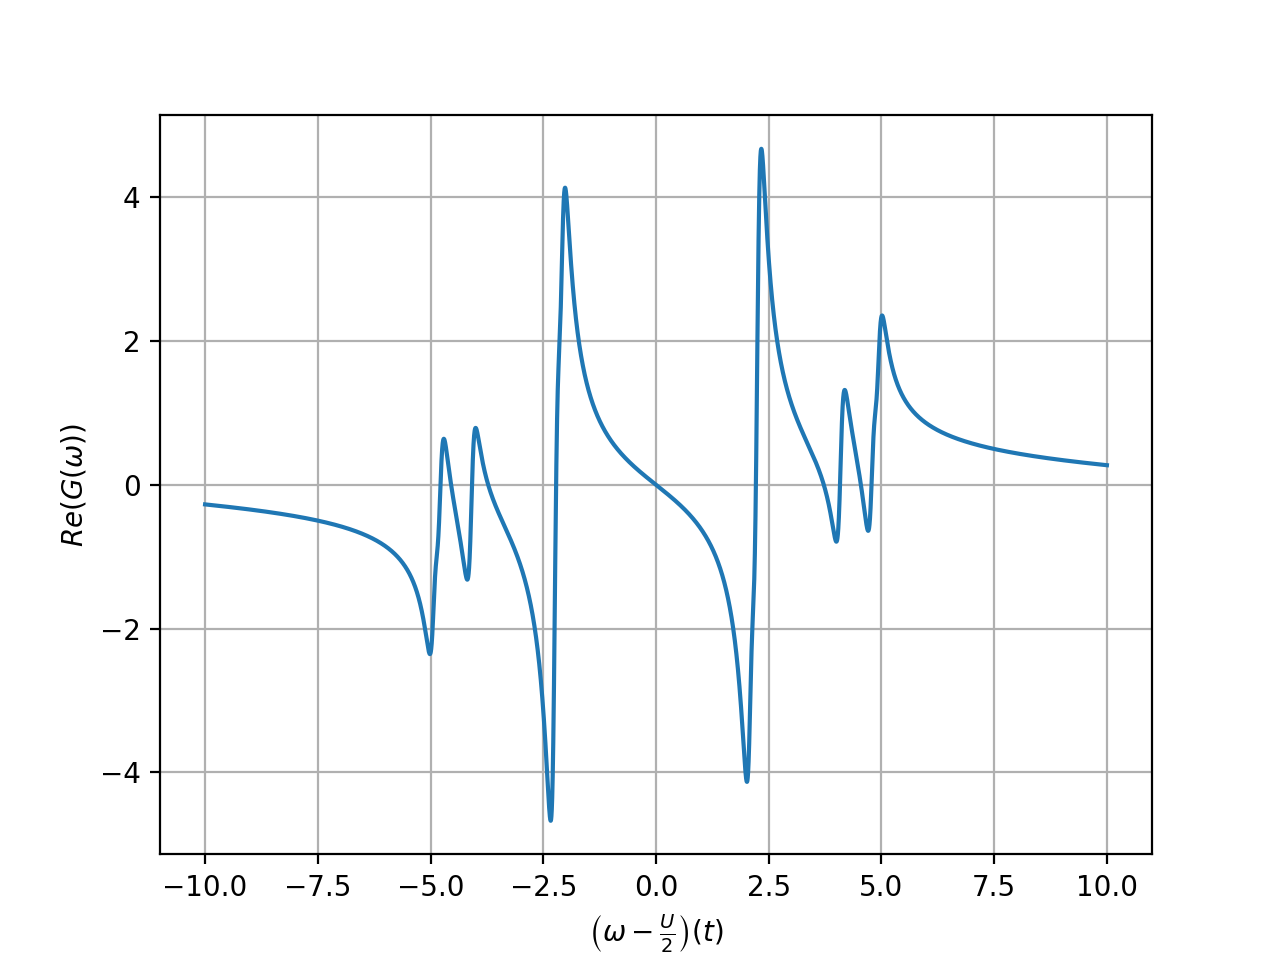
\includegraphics[max width=0.49\linewidth]{lanczosHubbard6U6Real.png}
    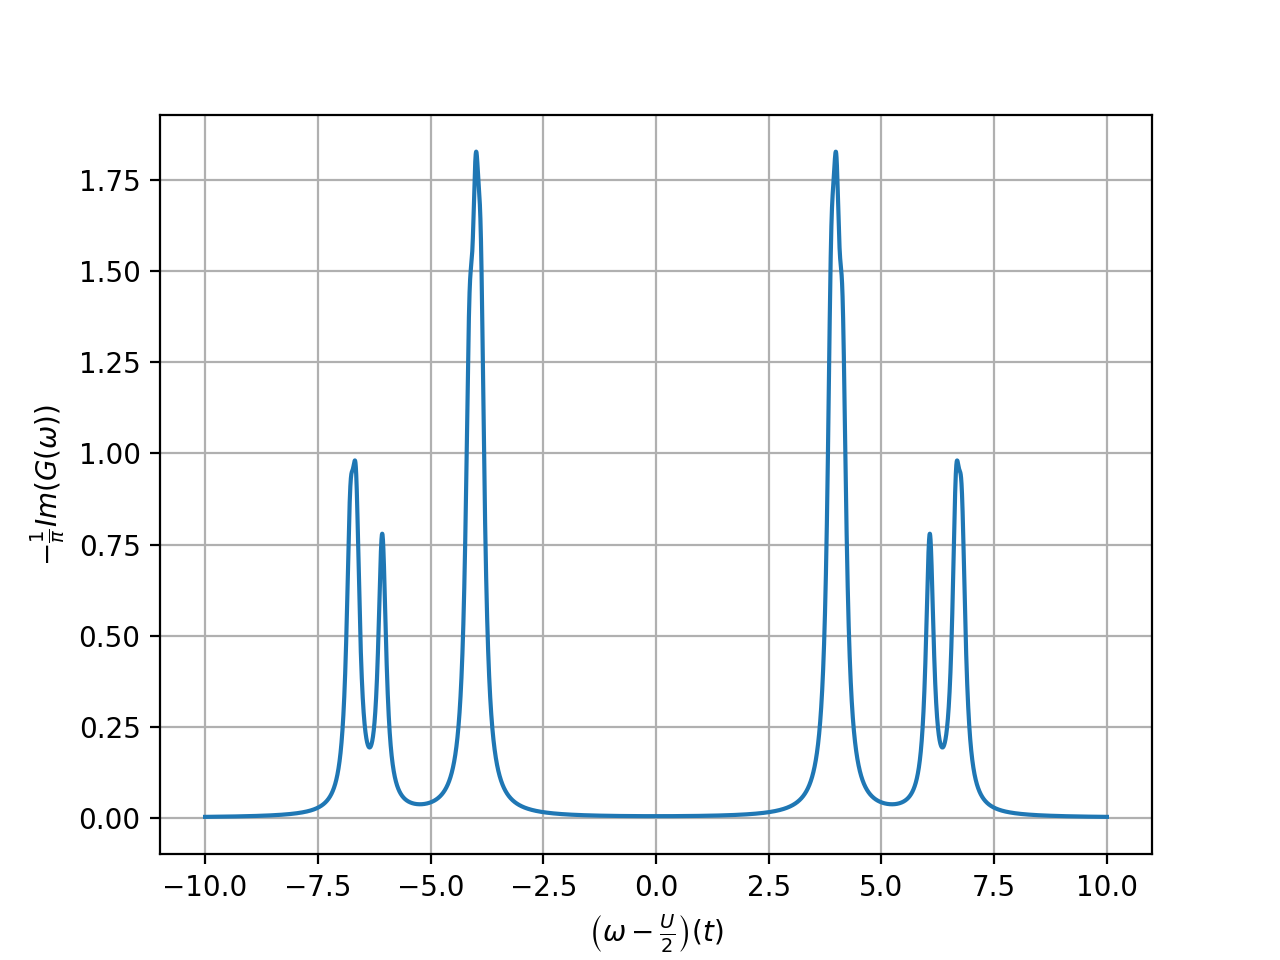
\includegraphics[max width=0.49\linewidth]{lanczosHubbard6U10Imag.png}
    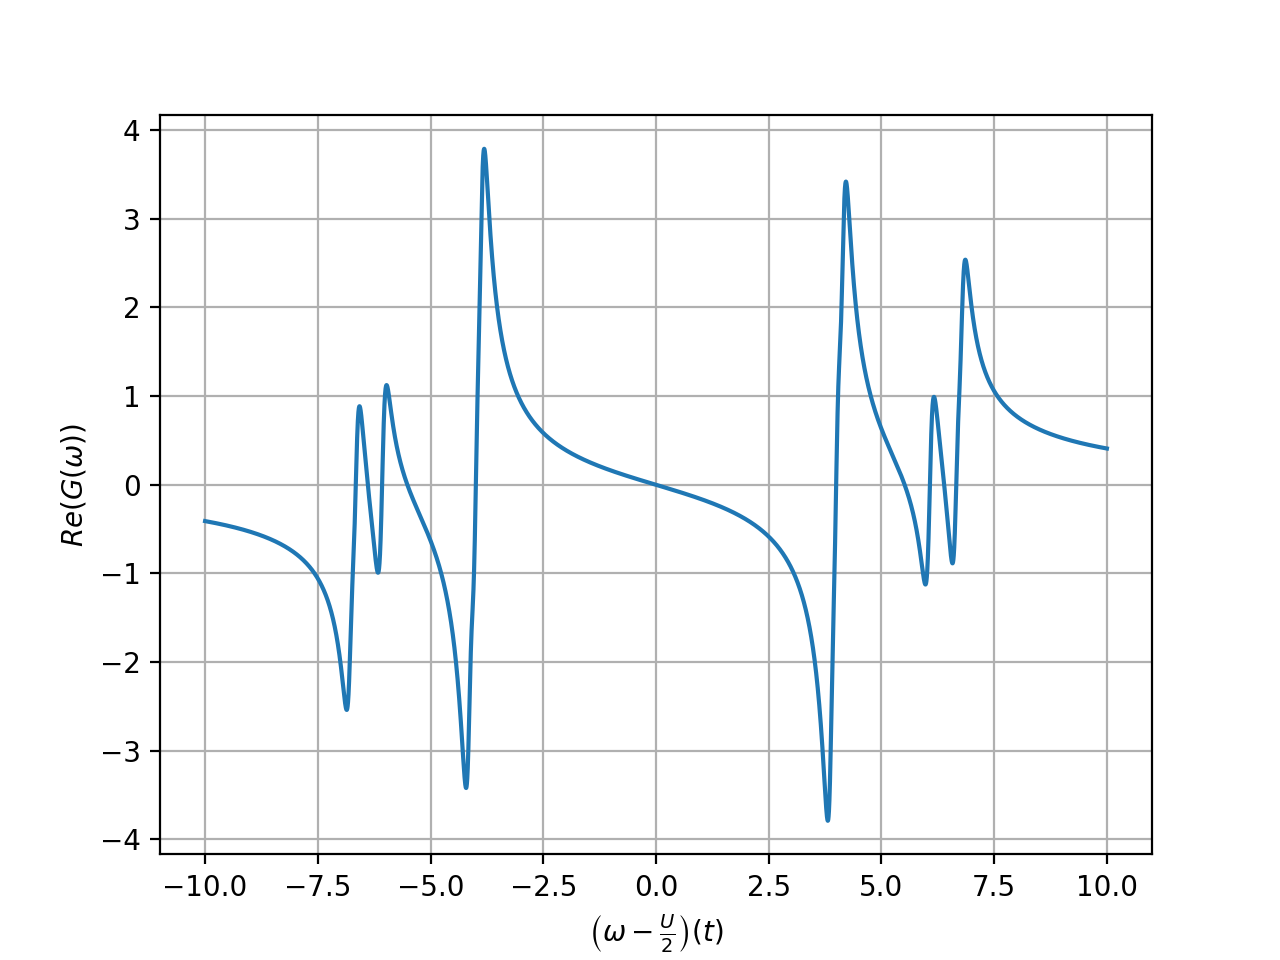
\includegraphics[max width=0.49\linewidth]{lanczosHubbard6U10Real.png}
  \end{center}
  \caption{Cadena de 6 núcleos, con condiciones de contorno periódicas y estado semillenado. Los valores del término de interacción van aumentando hacia abajo, siendo $U = 0t$, $U = 6t$ y $U = 10t$.}
  \label{fig:hubbardTransition6}
\end{figure}

En esta figura se puede observar muy bien la transición que sufre la cadena. Partimos de una única banda, con un pico en el centro, a formar dos bandas muy claras, separadas por un gap muy grande, que viene controlado por el valor de $U$.

La apertura de este gap implica un cambio de propiedades:
\begin{itemize}
  \item \textit{Aparecen dos bandas}. El sistema, que sin interacción sólo formaba una banda, ahora pasa a formar dos bandas muy definidas, apareciendo un gap de energías prohibidas muy claro.
  \item \textit{Perdemos la conductividad.} Ahora, la banda inferior está totalmente llena, y el gap es tan grande que los electrones no pueden saltar fácilmente de una a otra banda (el término de hopping resulta insuficiente para hacerlos saltar). De este modo, hemos encontrado que nuestro material pasa a ser un aislante al introducir una interacción.
\end{itemize}

Podríamos pensar que, al considerar muchas más partículas, los niveles pasan a ser bandas continuas y podríamos tener conducción aun así por movimiento de los electrones en la banda, puesto que los átomos están semillenos. Para responder a esto, recordemos rápidamente el término de interacción en el hamiltoniano de Hubbard:
$$
H_{int} = \sum_x U_x c^{\dagger}_{x\uparrow}c^{\dagger}_{x\downarrow}c_{x\downarrow}c_{x\uparrow}
$$

Efectivamente, los estados con muchos electrones aparejados son estados pertenecientes a la banda superior, puesto que tienen una penalización $U>0$ por emparejarse. En general, los estados en la banda inferior van a ser con electrones desapareados, de la forma:
$$
\begin{array}{ccccc}
  |\uparrow, \downarrow, \downarrow, \uparrow, \downarrow, \uparrow\rangle & \hspace{0.05\linewidth} & |\uparrow, \uparrow, \uparrow, \downarrow, \downarrow, \downarrow\rangle & \hspace{0.05\linewidth} & |\uparrow, \uparrow, \downarrow, \downarrow, \uparrow, \downarrow\rangle
\end{array}
$$

Es decir, no es sólo que exista una gran separación en las bandas, si no que, además, moverse dentro de la banda inferior es muy costoso. Este coste es debido a que para moverse los electrones deben de formar pares, o bien hacer hopping, que en la configuración actual está configurado para ser positivo, por lo que penaliza el movimiento dentro de la cadena. En resumen, moverse cuesta energía, así como formar pares, por lo que los electrones quedan quietos.

Para ver que, efectivamente, al hacer $U$ muy grande, no se forman pares de electrones $\uparrow\downarrow$, vamos a evaluar la siguiente expresión:
\begin{equation}
  P = \sum_i\langle\psi_0|c_{i\downarrow}^{\dagger}c_{i\uparrow}^{\dagger}c_{i\uparrow}c_{i\downarrow}|\psi_0\rangle
\end{equation}

Aquí $|\psi_0\rangle$ es el estado fundamental de nuestro sistema, y el número $P$ representa el número promedio de pares. Vamos a estudiar de nuevo el dímero de Hubbard por simpleza. Representemos este valor en varios casos en la figura \ref{fig:probPairsPos}
\begin{figure}[h!]
  \begin{center}
    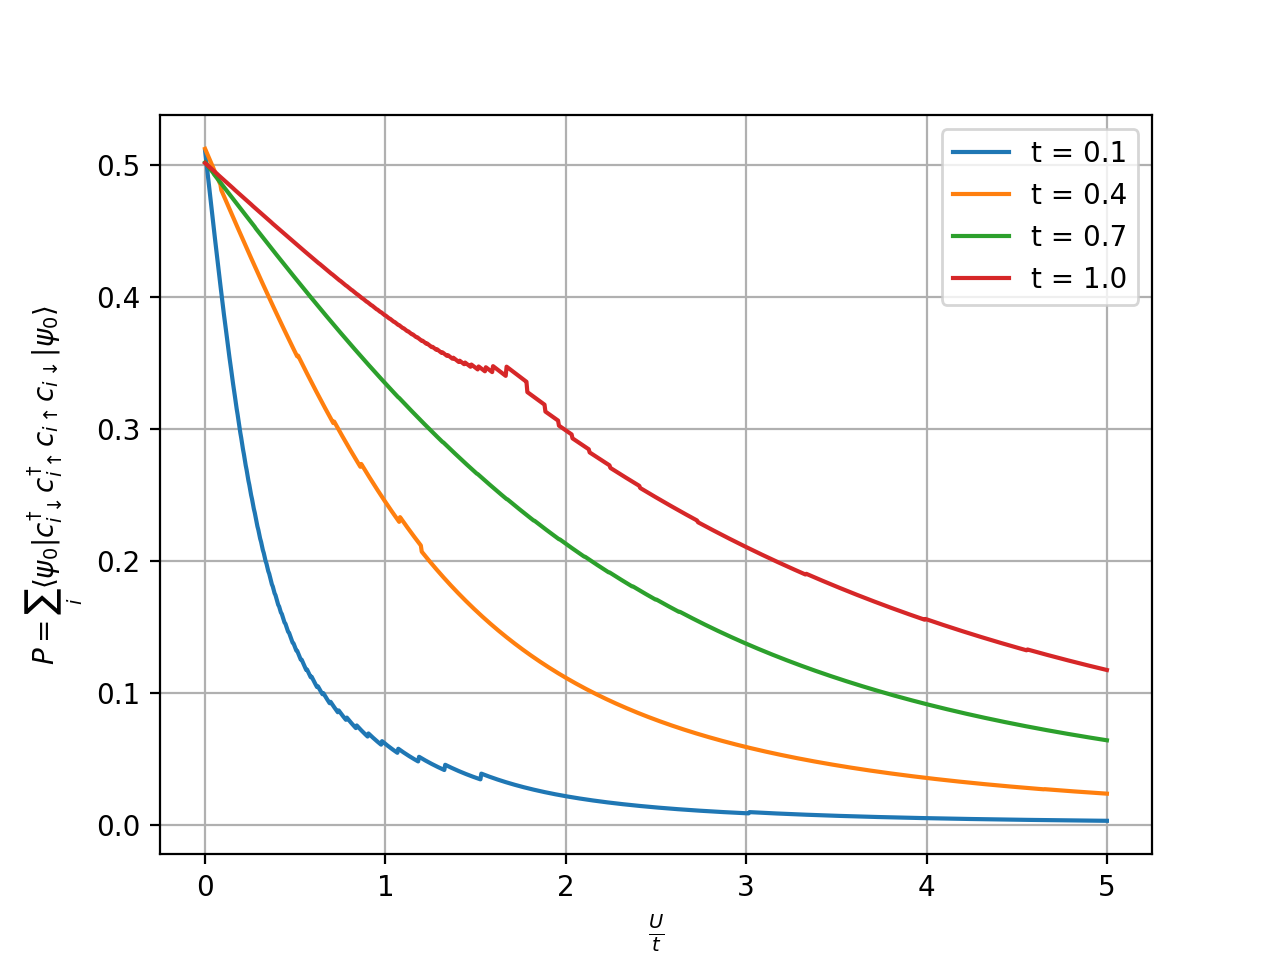
\includegraphics[max width=\linewidth]{ProbabilityPairsPositive.png}
  \end{center}
  \caption{Número promedio de pares en función del valor de $U$ respecto a $t$, representado para varios valores de $t$, donde se observa el mayor número de pares al aumentar $t$ y disminuir $U$.}
  \label{fig:probPairsPos}
\end{figure}

El comportamiento que esperábamos al aumentar $U$ es que no se forman pares, debido a la penalización energética. Sin embargo, ¿tiene sentido ese valor de 0,5 en $U = 0$? Vamos a pensar en los posibles microestados del sistema en este caso:
$$
\begin{array}{cccc}
  |\uparrow, \downarrow\rangle & |\uparrow\downarrow, 0\rangle & |\downarrow, \uparrow\rangle & |0, \uparrow\downarrow\rangle
\end{array}
$$ 

Es decir, mediremos alguna de estas combinaciones siempre. De este modo, el estado fundamental será una combinación lineal de estos estados, y como $U = 0$, podemos pensar que son equiprobables. Pensemos que en este caso nuestro hamiltoniano es:
$$
H_0 = \sum_{x, y, \sigma}t_{xy}c^{\dagger}_{x,\sigma}c_{y,\sigma}
$$

Fijémonos en la referencia \cite{GreeneDiniz2024}, en la ecuación (19) de la referencia, se menciona que el estado fundamental del dímero tiene estos cuatro estados como equiprobables. Es fácil comprobar que esto es así tomando los autovectores de la matriz $t_{ij}$, y al no ser un sistema correlacionado hacer un producto de ambos estados. Para nuestro caso, los autovectores de un electrón de la matriz son:
\begin{equation}
  \begin{array}{cc}
    |\psi_1\rangle = \frac{1}{\sqrt{2}}\left(|01\rangle + |10\rangle\right) & |\psi_2\rangle = \frac{1}{\sqrt{2}}\left(|01\rangle - |10\rangle\right)
  \end{array}
\end{equation}

Y para hacer los autoestados hay que tomar ambos electrones en el estado fundamental, que es el autovector con autovalor asociado más bajo, siendo este $|\psi_1\rangle$. Tomandolos así, el estado fundamental de dos electrones será:
$$
|\psi_0\rangle = \frac{1}{2}(|\uparrow, \downarrow\rangle + |\uparrow\downarrow, 0\rangle + |\downarrow, \uparrow\rangle + |0, \uparrow\downarrow\rangle)
$$

Por lo que las probabilidades de cada estado son equiprobables, y entonces, el número medio de pares es de $\frac{1}{2}$ para el caso de $U = 0$. El mismo resultado que habíamos calculado numéricamente. Nuevamente, nos sirve como control de calidad para el programa.

Finalmente vamos a estudiar los casos de carga desequilibrada, es decir, vamos a eliminar y añadir un electrón. De este modo, tendremos el dímero cargado positiva o negativamente. Vamos a comenzar con el caso del dímero cargado positivamente, observemos la figura \ref{fig:positiveDimer}
\begin{figure}[h!]
  \begin{center}
     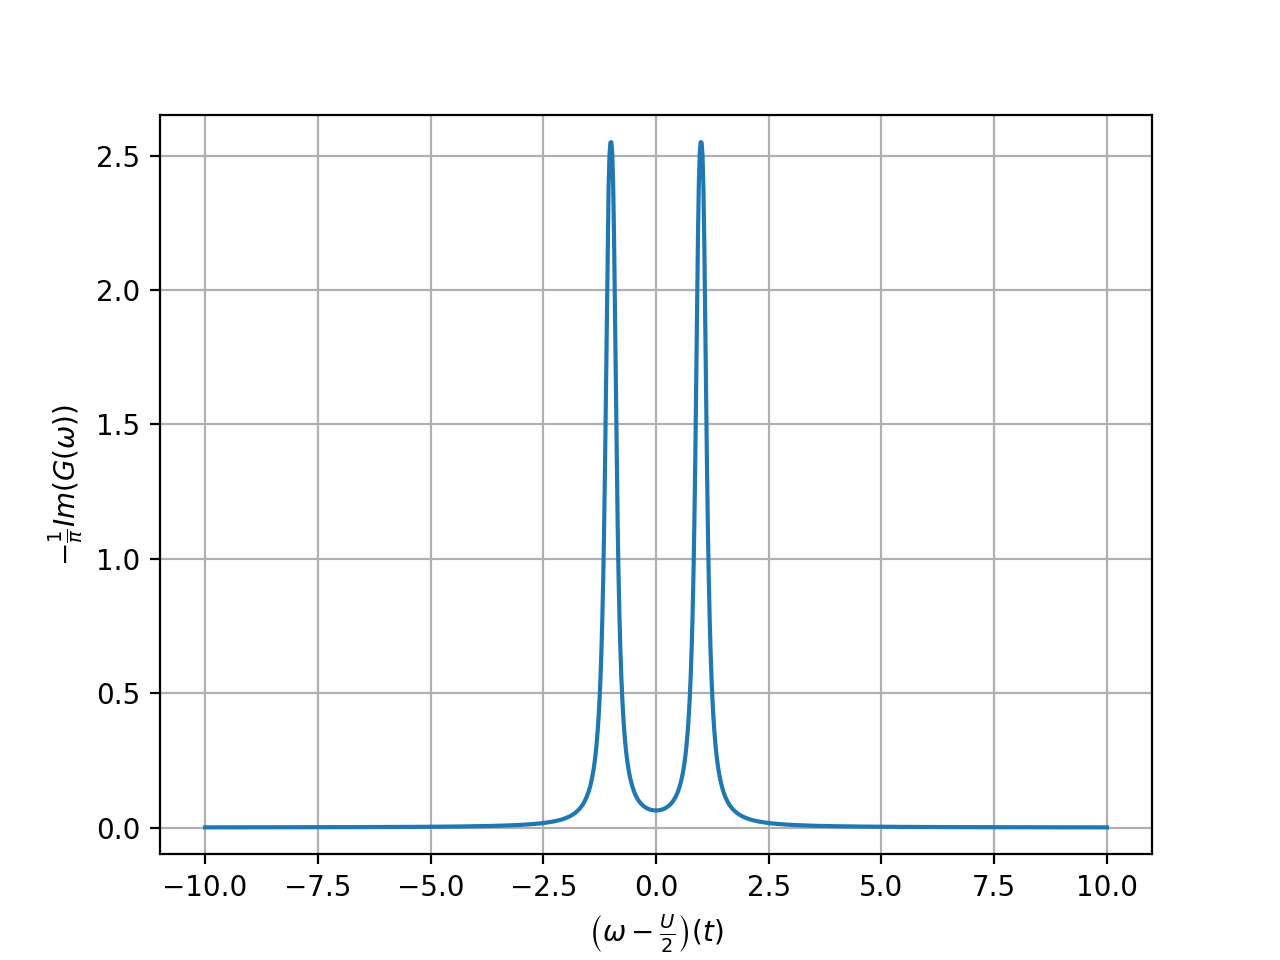
\includegraphics[max width=0.49\linewidth]{lanczosHubbard2PosU0Imag.png}
     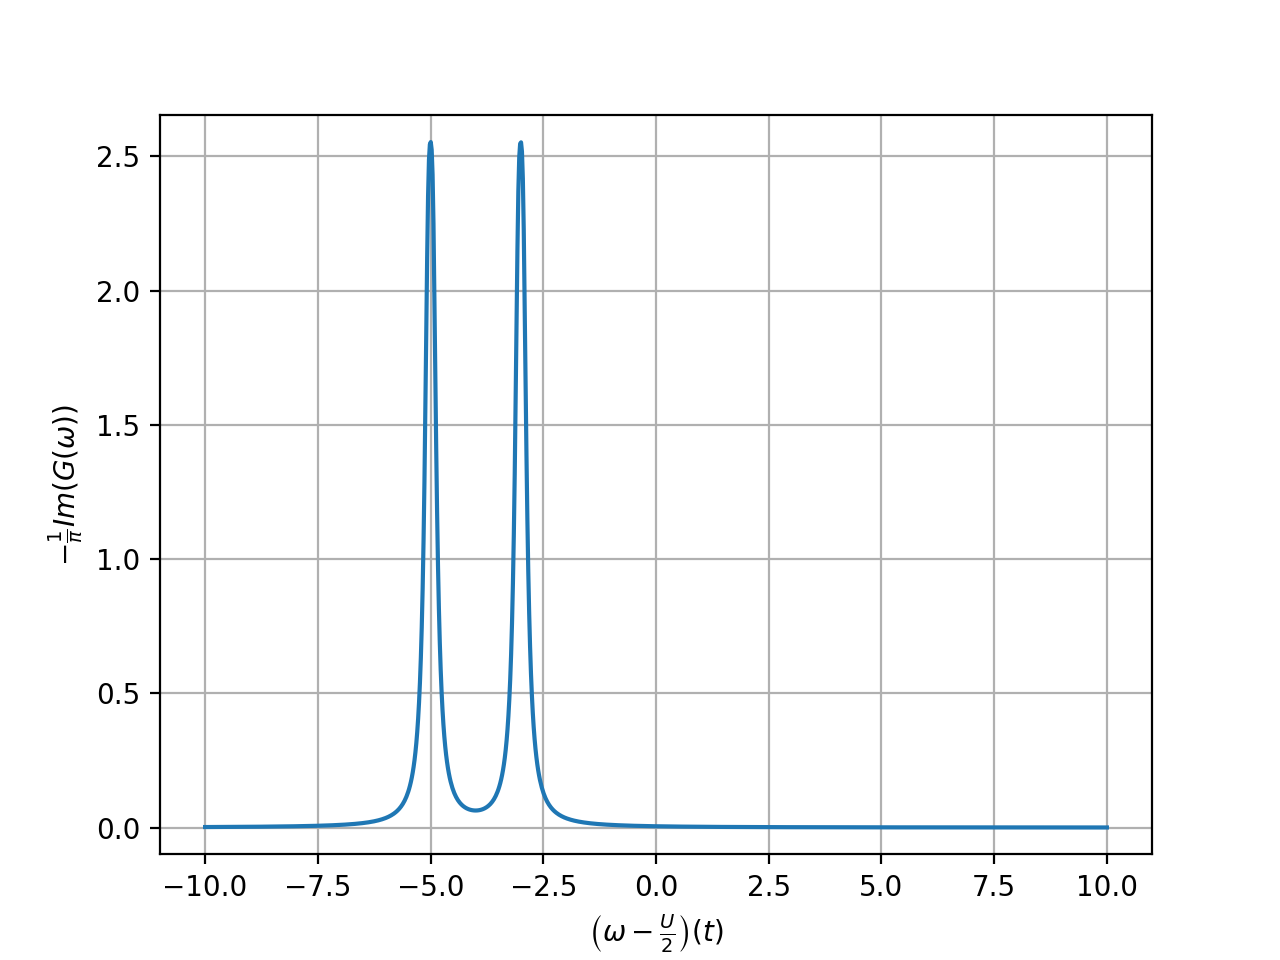
\includegraphics[max width=0.49\linewidth]{lanczosHubbard2PosU8Imag.png}
  \end{center}
  \caption{Densidad de estados del dímero cargado positivamente para los casos $U = 0$ y $U = 8$ eliminando el electrón de spin down.}
  \label{fig:positiveDimer}
\end{figure}

Como se puede observar, se forman dos picos. Además, se puede observar el desplazamiento de los picos. Sin embargo, en este caso el material sigue siendo conductor y no ocurre un desdoblamiento de las bandas. Sí que se desplazan los niveles de energía, pero no se pierden las propiedades de conducción. Podemos observar también el número de pares, pero al haber sólo un electrón, serán cero.

Analicemos a continuación el dímero cargado negativamente, así que añadiremos un electrón con spin down. Las funciones de Green que se obtienen son las mismas que en el caso de carga positiva, y, al tener dos electrones en la posición down siempre se va a ver forzado a formar un par, por lo que el número promedio de pares es uno. Todos estos resultados se pueden ver en la figura \ref{fig:negativeDimer}.
\begin{figure}[h!]
  \begin{center}
    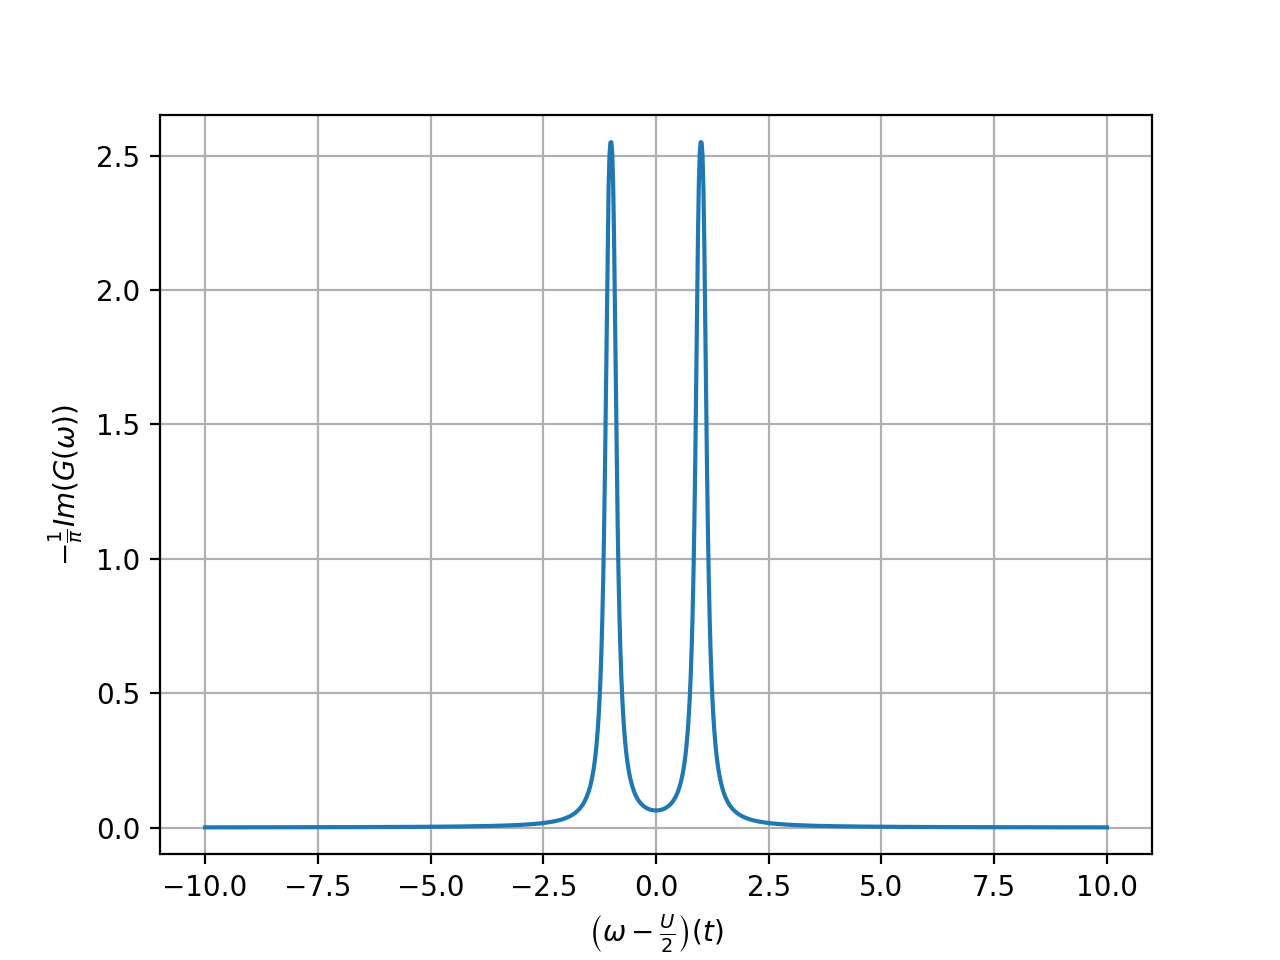
\includegraphics[max width=0.49\linewidth]{lanczosHubbard2NegU0Imag.png}
    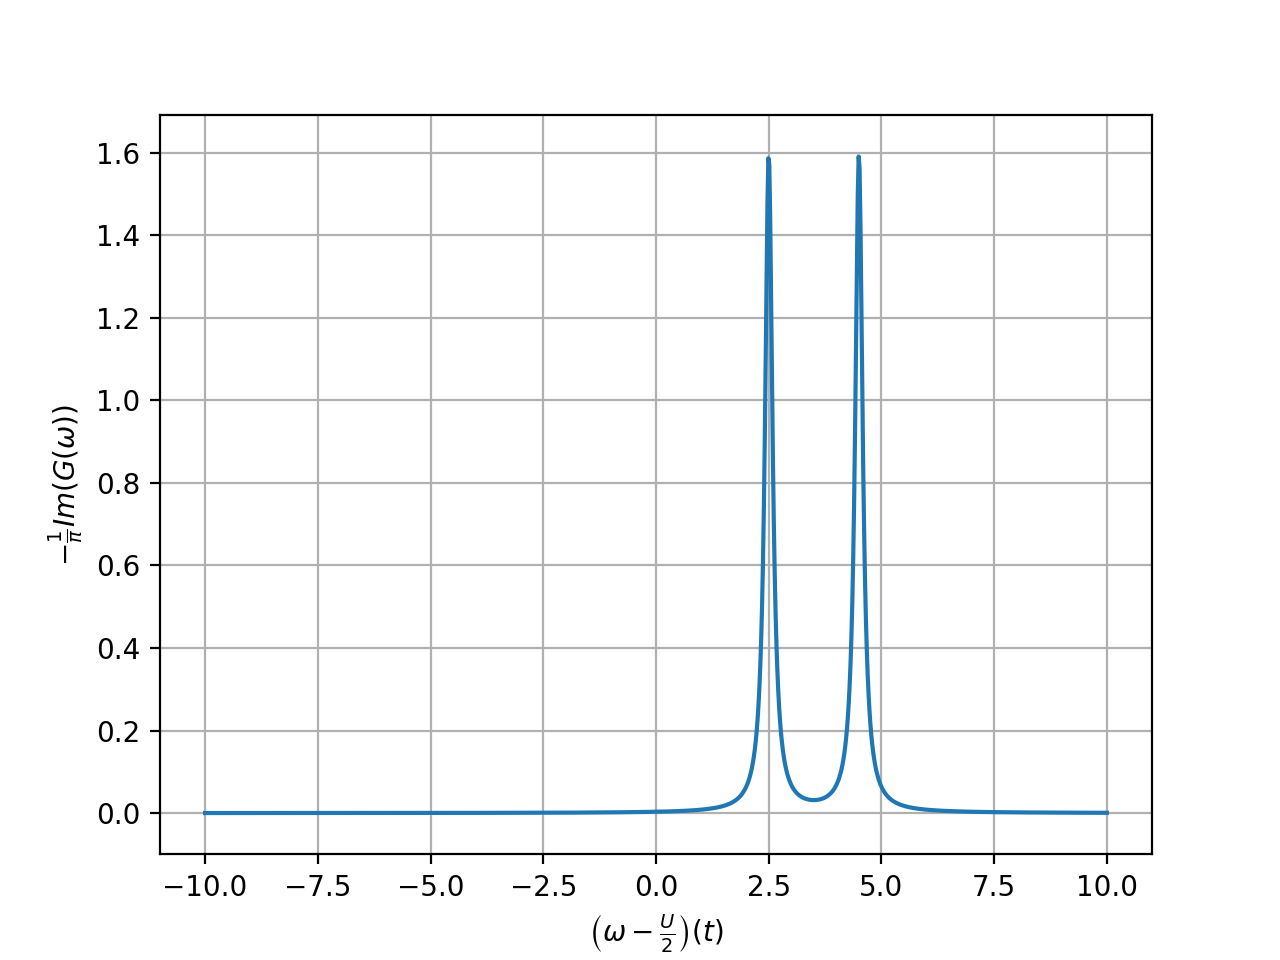
\includegraphics[max width=0.49\linewidth]{lanczosHubbard2NegU8Imag.png}
  \end{center}
  \caption{Densidad de estados obtenida para el caso del dímero cargado negativamente.}
  \label{fig:negativeDimer}
\end{figure}

Efectivamente, en el caso cargado negativamente, tampoco se pierde la conductividad al aumentar $U$, pero ahora los niveles de energía suben, y la partícula está forzada a formar un par. Todo funcionando tal y como esperábamos.
\subsubsection{Superconductividad}

Toda la sección anterior hemos estado estudiando un caso en que $U > 0$, sin embargo, exigir $U < 0$ tiene consecuencias interesantes. Supongamos que ahora los pares de electrones interactúan atractivamente, esto es un caso imaginario, pero interesante. Para ello, necesitamos observar primero la formación de pares para valores de $U$ negativos. La representación del número promedio de pares está en la figura \ref{fig:pairAverage}.
\begin{figure}[h!]
  \begin{center}
    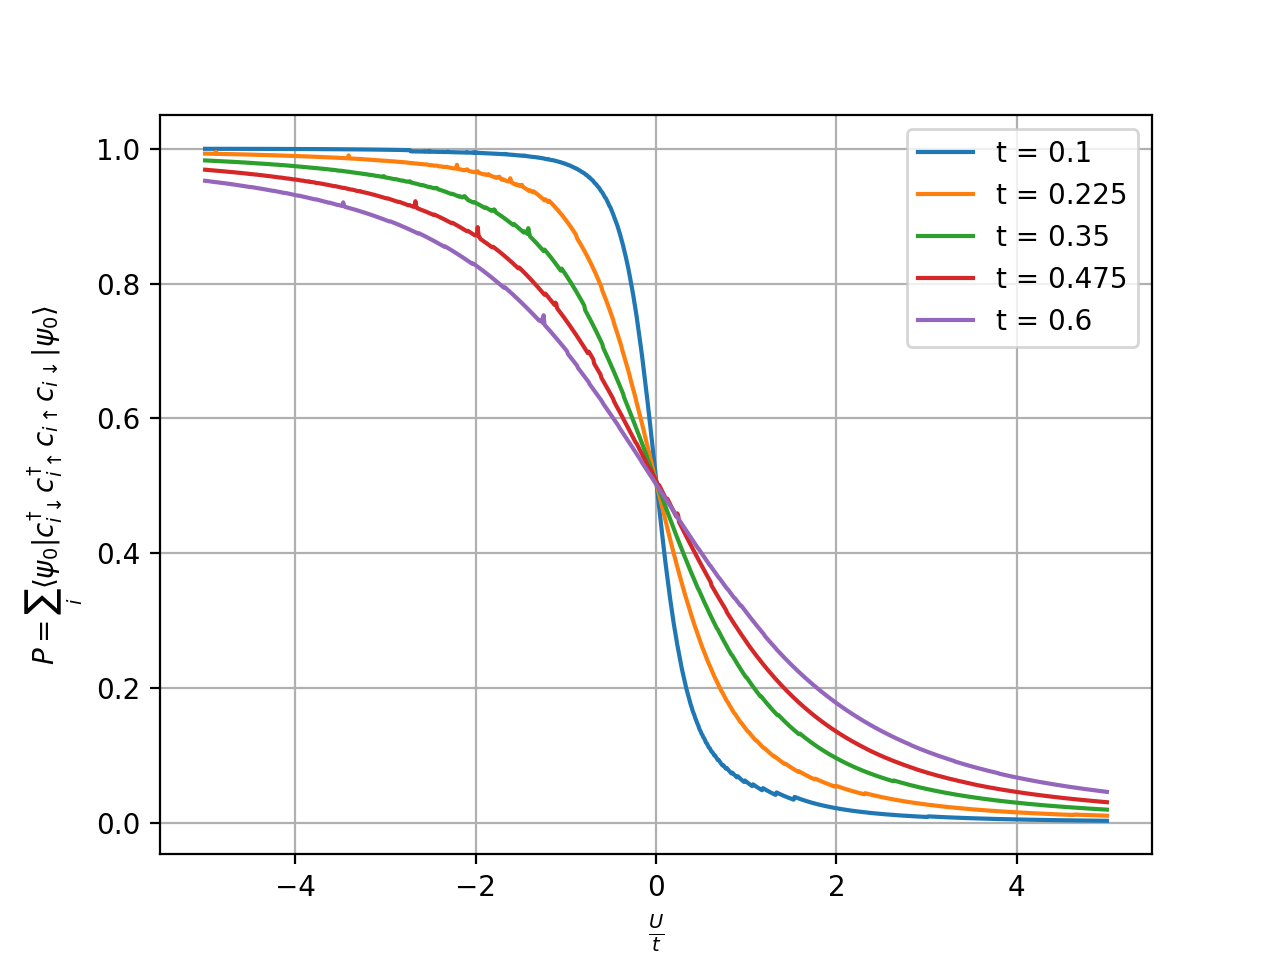
\includegraphics[max width=\linewidth]{ProbabilityPairsAll.png}
  \end{center}
  \caption{Promedio de pares formados en función de $U$ y de $t$ para el dímero de Hubbard con un estado electrónico de semillenado.}
  \label{fig:pairAverage}
\end{figure}

La forma de la densidad de estados no cambiará para este caso, pero sí que cambia el número promedio de pares. Cuanto mayor es el módulo de $U$, el número de pares tiende al máximo posible, en el límite $|U| \gg |t|$ se cumplirá que $P \approx 1$.

Es decir, nuestro estado fundamental serán estados de pares mayoritariamente, puesto que ahora, la banda inferior agrupa a estados con los electrones apareados.

Estos pares son característicos de la superconductividad de tipo BCS. Ocurren en sitios con forma $\uparrow\downarrow$ y tienen comportamiento bosónico, puesto que cada par tiene un spin total $S = 0$. En efecto, al hacer la interacción $U$ mucho mayor en módulo respecto al hopping, $t$, hemos conseguido un estado fundamental en el que se forman pares electrón-electrón, para el caso del semillenado, $\frac{N}{2}$.

Y como los electrones se organizan formando pares en el estado fundamental, podremos comprobar que esto cumple el teorema de Lieb \cite{MielkeHubbard}, puesto que el estado fundamental tiene spin total $S = 0$.

Podemos concluir que, en un modelo con $U < 0$, aparecerá en el material una superconductividad. En la densidad de estados se puede ver ese gran hueco, característico de la interacción, y además la formación de pares up-down da lugar a la superconductividad de tipo BCS, aunque seguimos necesitando una descripción de la interacción electrón-fonón, que es la que modelizaría el término de Hubbard negativo. Se puede leer más sobre esta superconductividad en la referencia \cite{Russenschuck:503603}.
\begin{figure}[h!]
  \begin{center}
    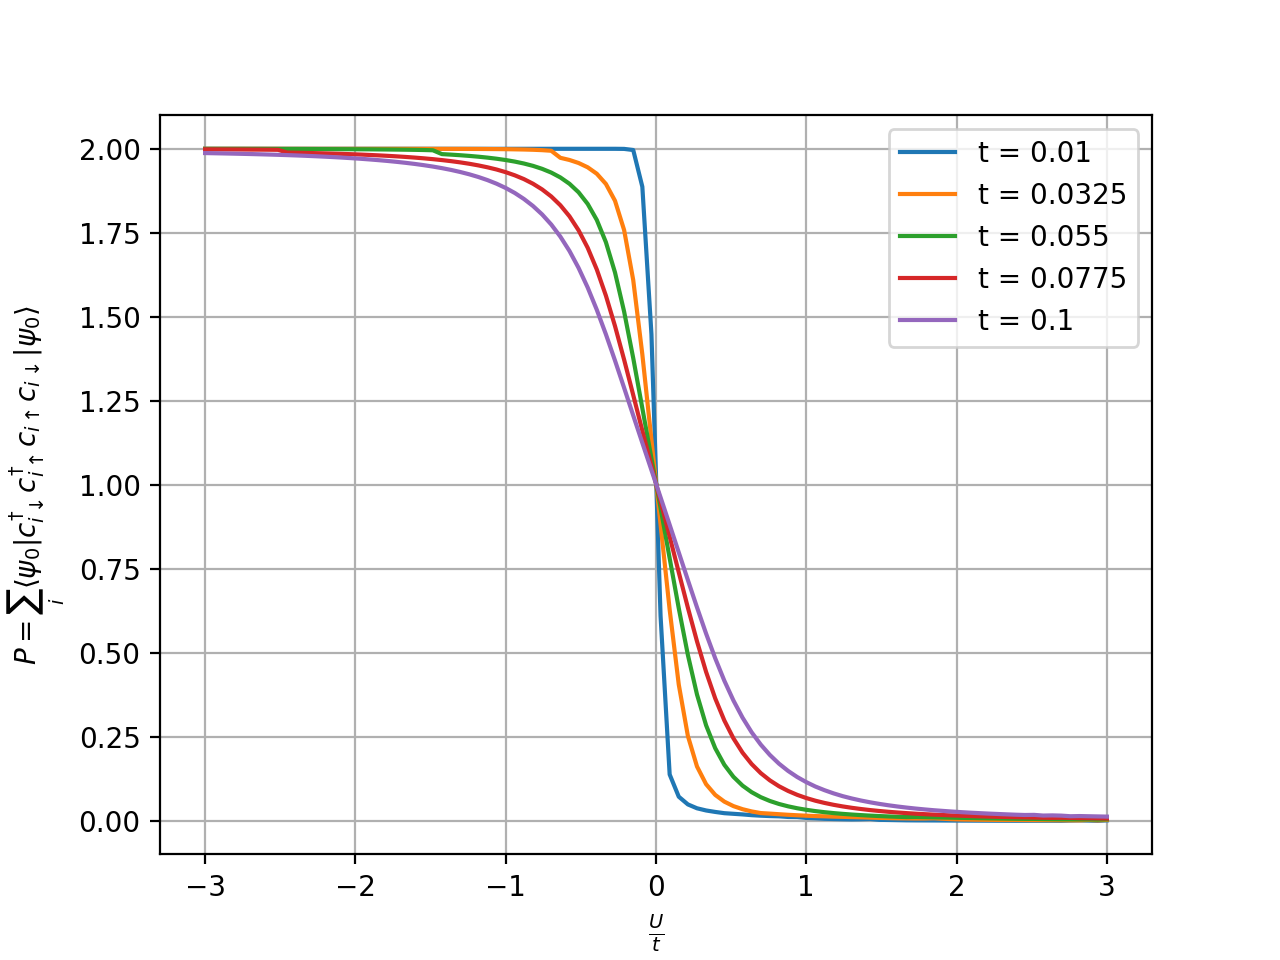
\includegraphics[max width=\linewidth]{ProbabilityPairsAll4.png}
  \end{center}
  \caption{Número medio de pares up-down en función del valor de $U$ para distintos valores de $t$ en una cadena de cuatro sitios con condiciones de contorno periódicas y un semillenado de electrones.}
\end{figure}

No debemos confundir estos pares con los pares de Cooper de la superconductividad, puesto que estos van a depender de la interacción con los fonones, siendo cuasi-partículas. Además, en este modelo modificado, estos pares electrón-electrón son muy especiales, puesto que son resistentes a defectos.

Imaginemos un defecto en nuestra cadena, esto estaría modelado por el hopping, $t$. Bien, pues como podemos ver, al alejarse tanto las bandas debido al término de Hubbard, el coste energético de romper un par es mucho mayor que el que puede ejercer un defecto sobre el estado fundamental. En otras palabras, los pares están protegidos frente a defectos gracias al gap en la densidad de estados que abre el término $U$.
\subsubsection{Tiempos de cálculo}

Vamos a dedicar esta última sección para demostrar el coste computacional de resolver el modelo de Hubbard con el algoritmo de Lanczos. Para ello, he representado, para un pequeño número de valores de $N$, el tiempo de cálculo. Sólo se toman cuatro puntos, puesto que para valores mayores de $N$ el programa convergía demasiado lento. Ver figura \ref{fig:calcTimes}
\begin{figure}[h!]
  \begin{center}
    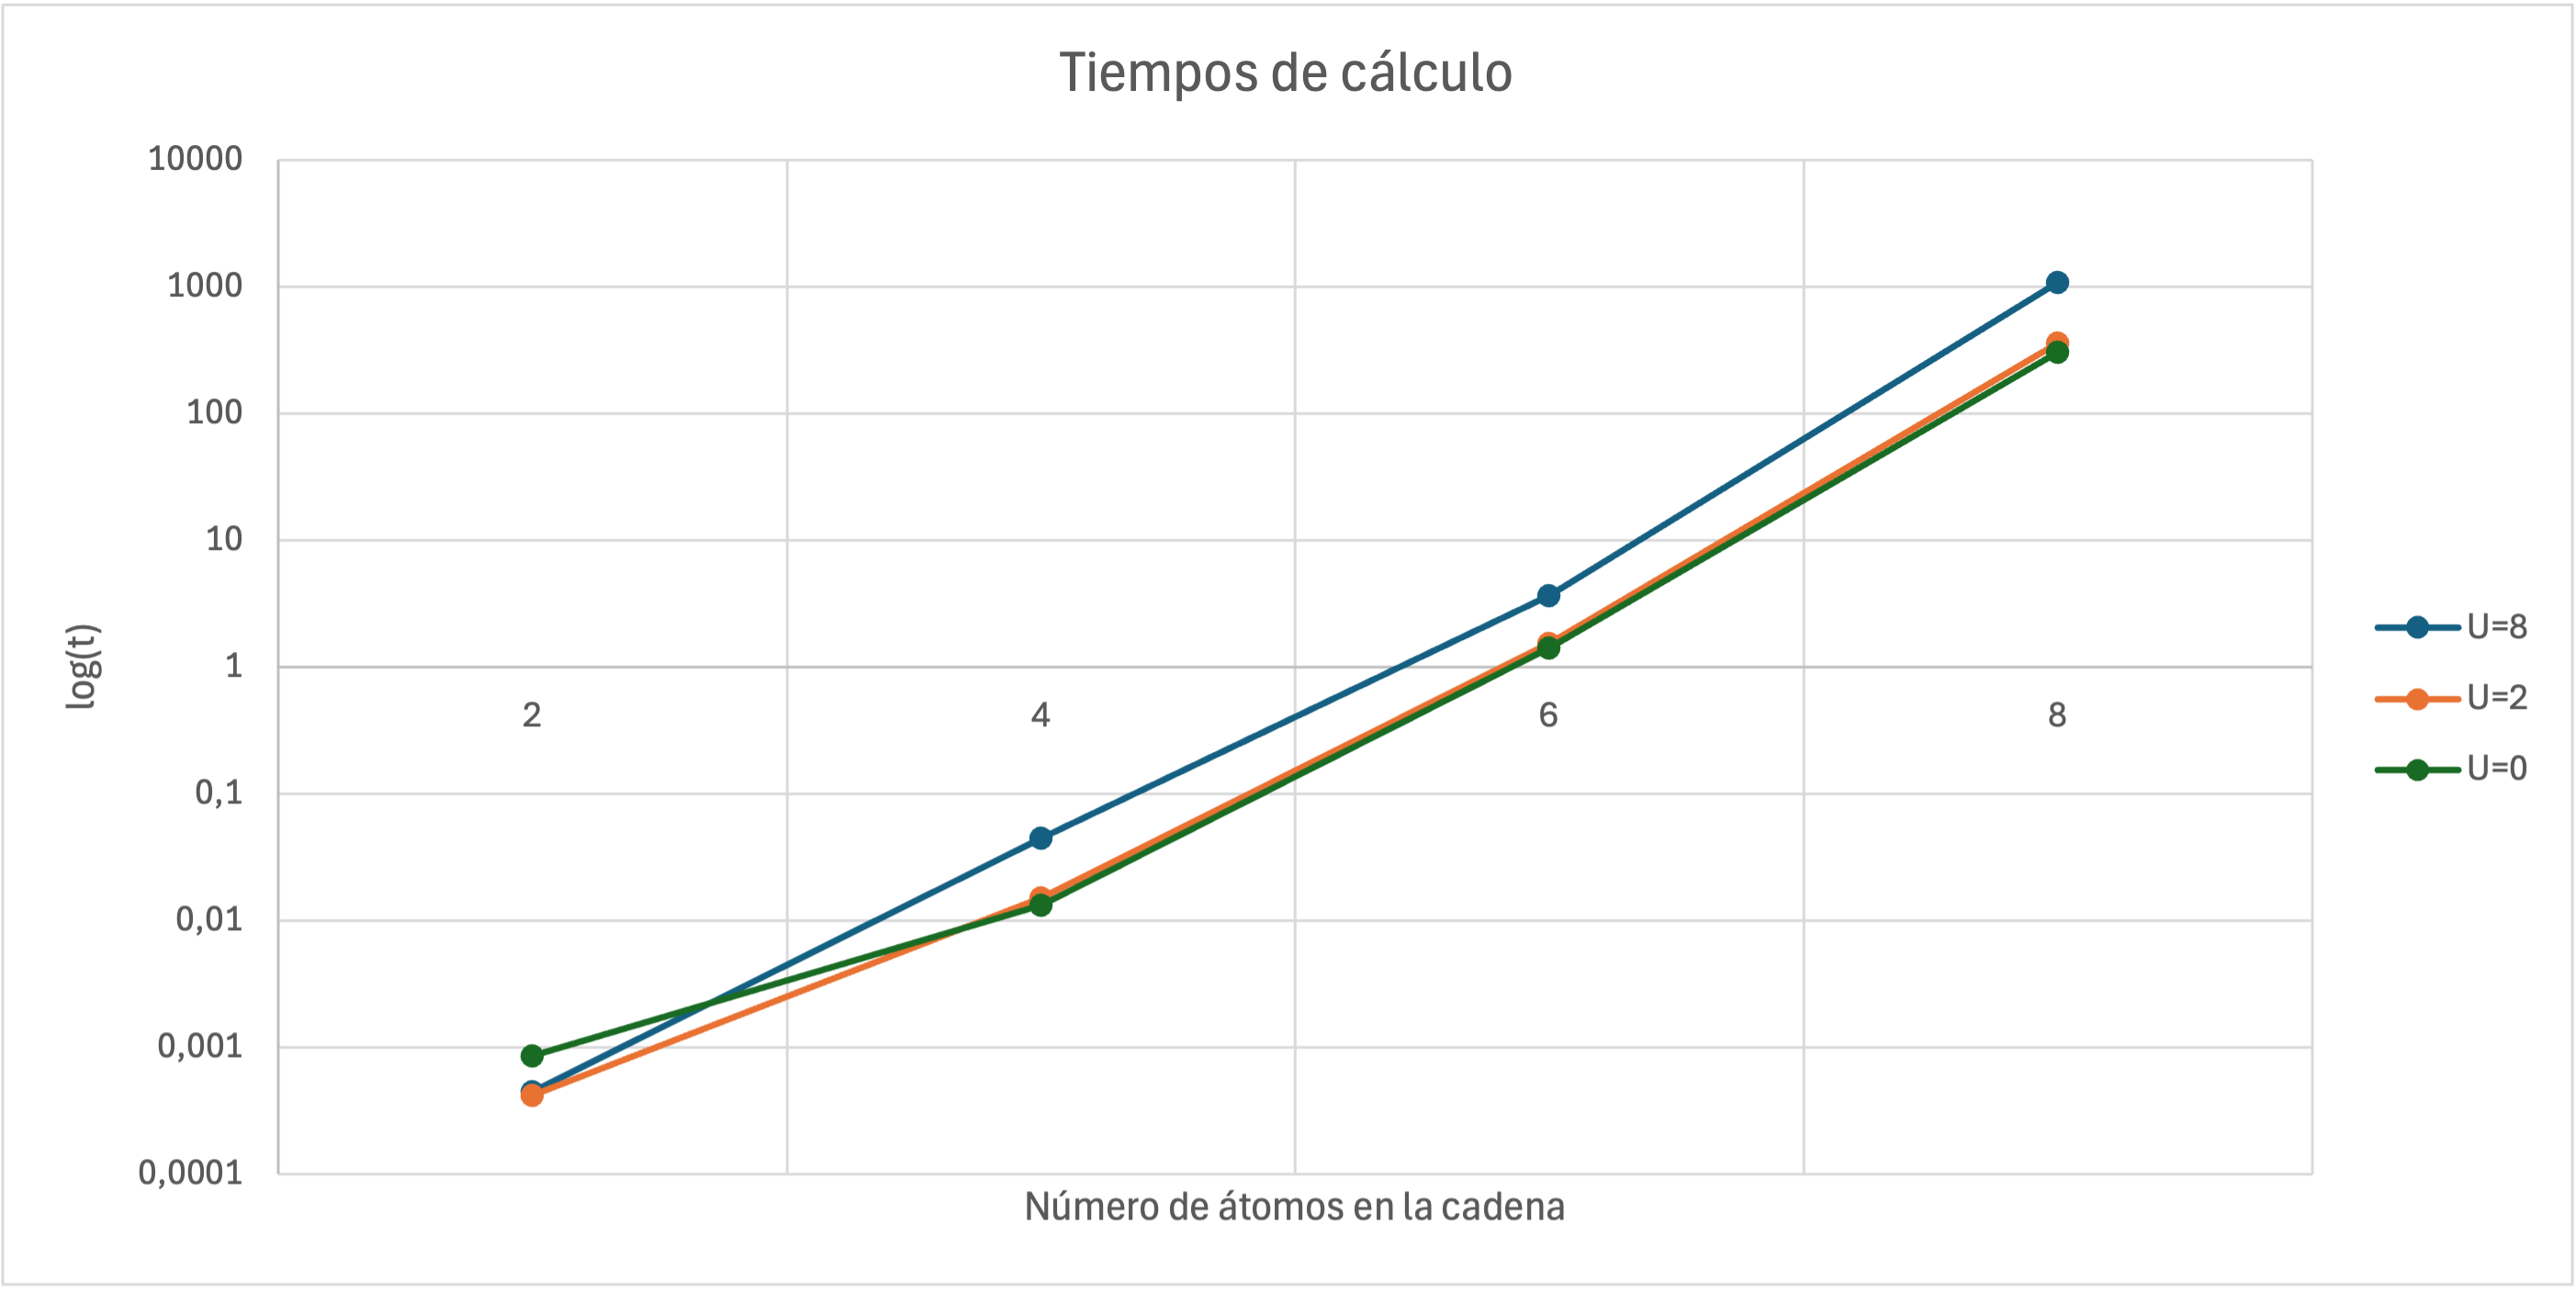
\includegraphics[max width=\linewidth]{tCalcs.png}
  \end{center}
  \caption{Tiempos de cálculo del programa, con escala logarítmica en el eje vertical y representados para varios valores del término de interacción $U$. En este caso el término de hopping, $t$, es positivo.}
  \label{fig:calcTimes}
\end{figure}

Podemos entender que la mejora en tiempo al usar $U=0$ es porque el ordenador tiene que hacer menos cálculos, sin embargo, para $U=2$ podríamos esperar el mismo tiempo que para $U=8$, así que, ¿por qué es considerablemente menor el tiempo? Para poder responder a esta pregunta con más precisión vamos a ver cómo convergen los métodos en función del paso, para ello representamos la diferencia de energías entre dos pases de Lanczos para los valores de la gráfica anterior. Observemos las figuras \ref{fig:convergenceGood} y \ref{fig:convergenceBad}.
\begin{figure}[h!]
  \begin{center}
    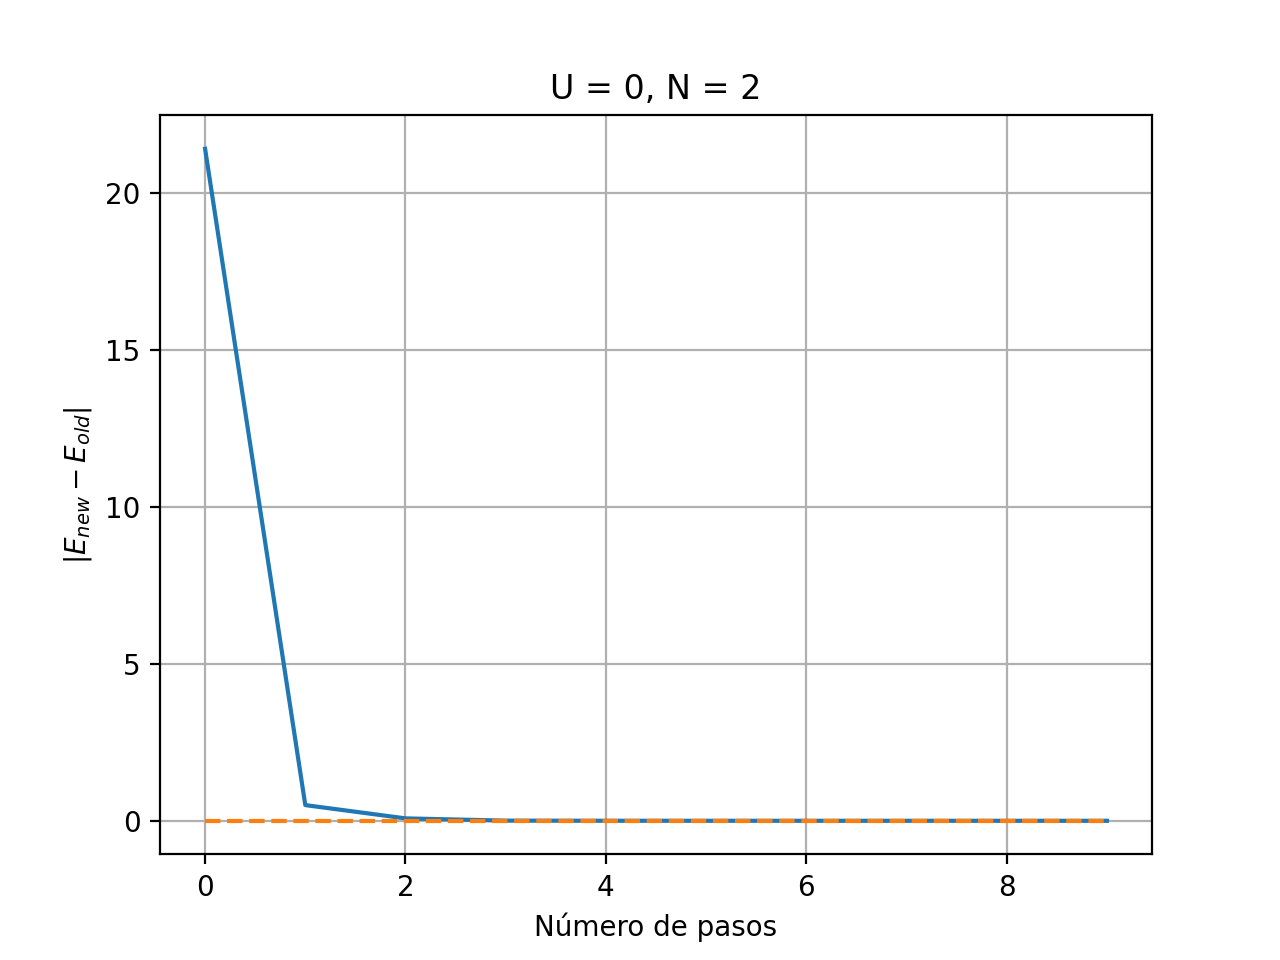
\includegraphics[max width=0.49\linewidth]{convergenceU0N2.png}
    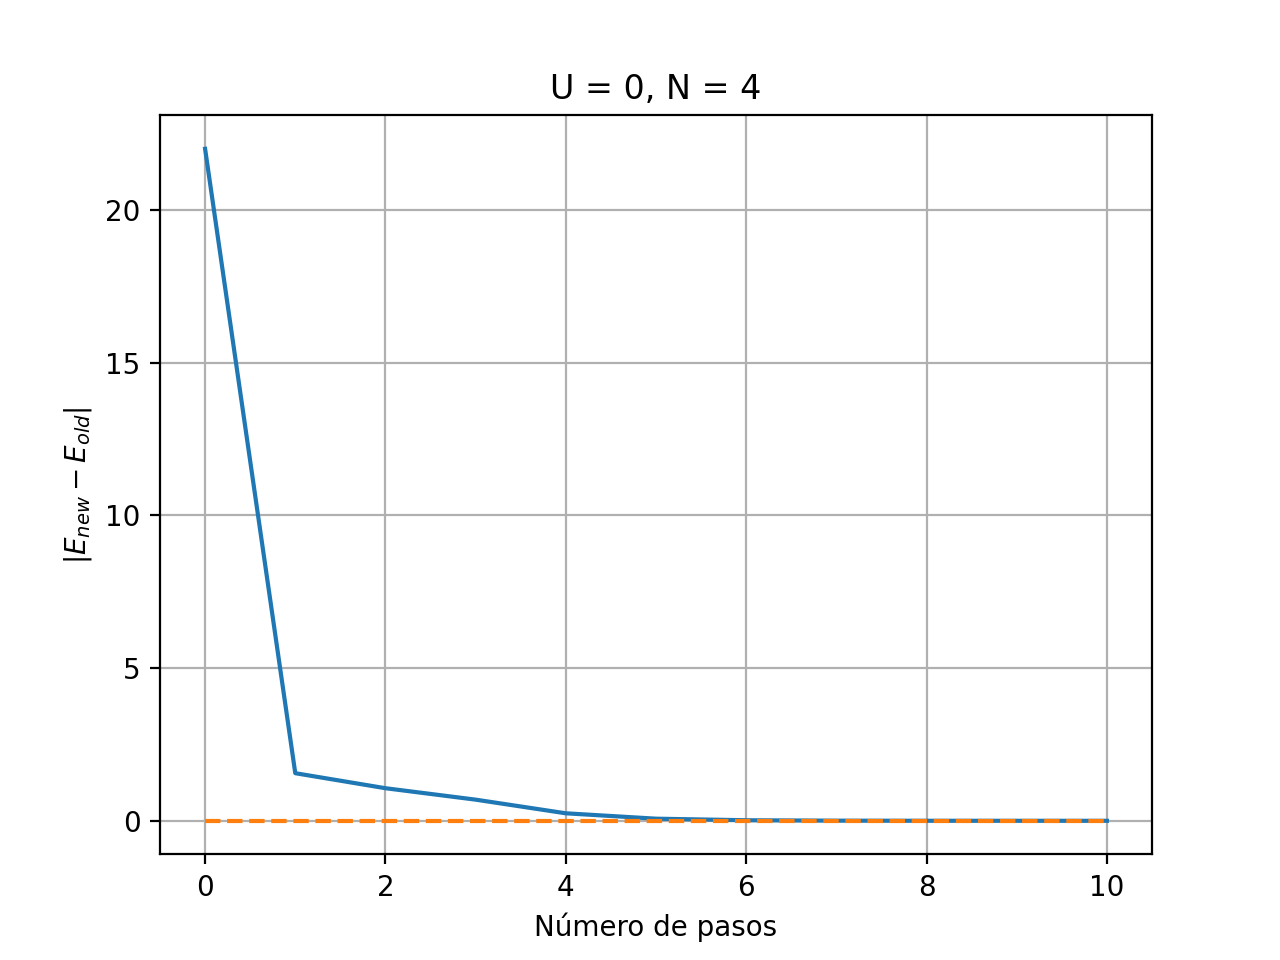
\includegraphics[max width=0.49\linewidth]{convergenceU0N4.png}
    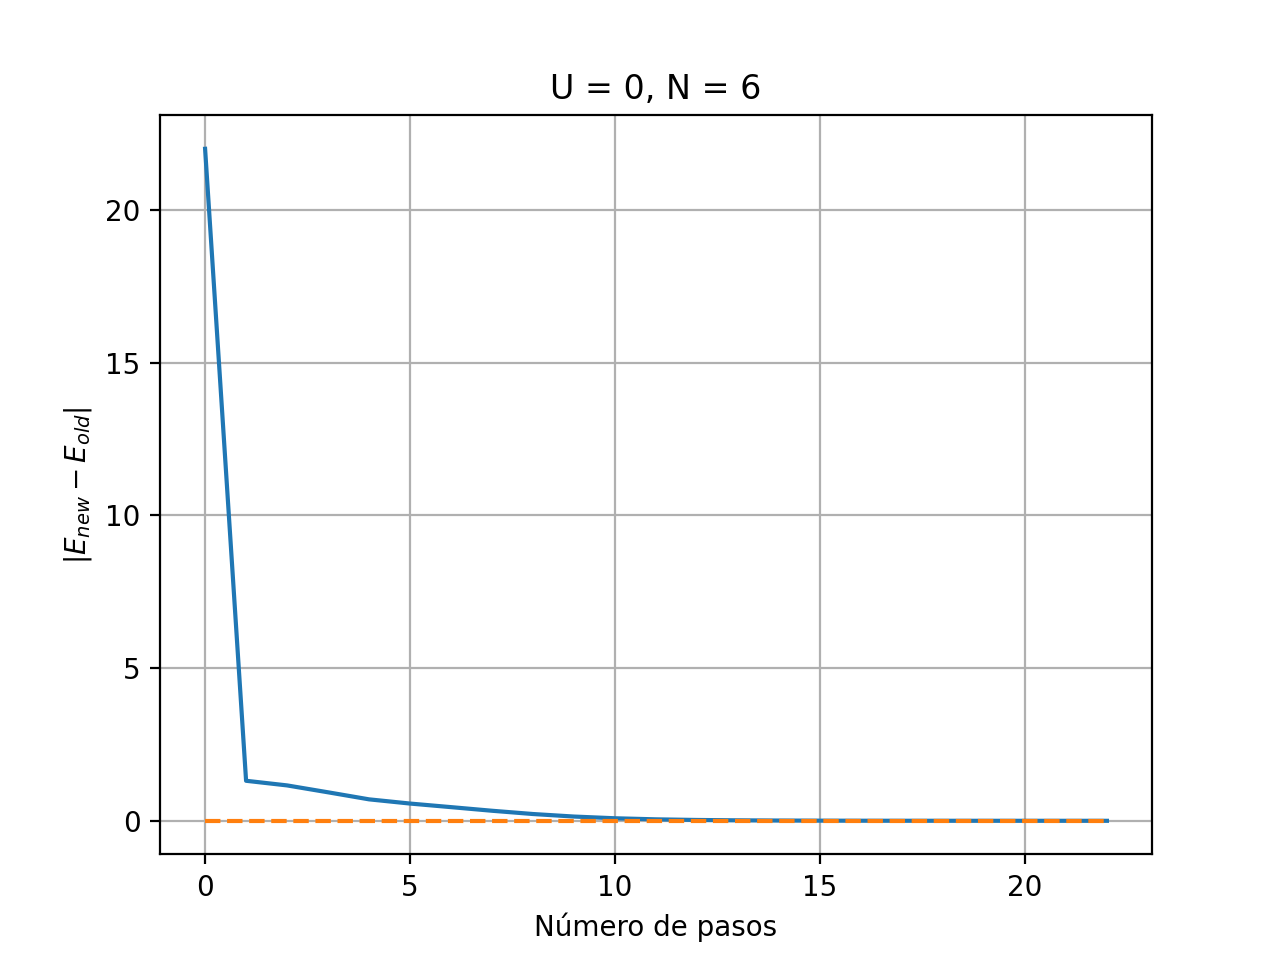
\includegraphics[max width=0.49\linewidth]{convergenceU0N6.png}
    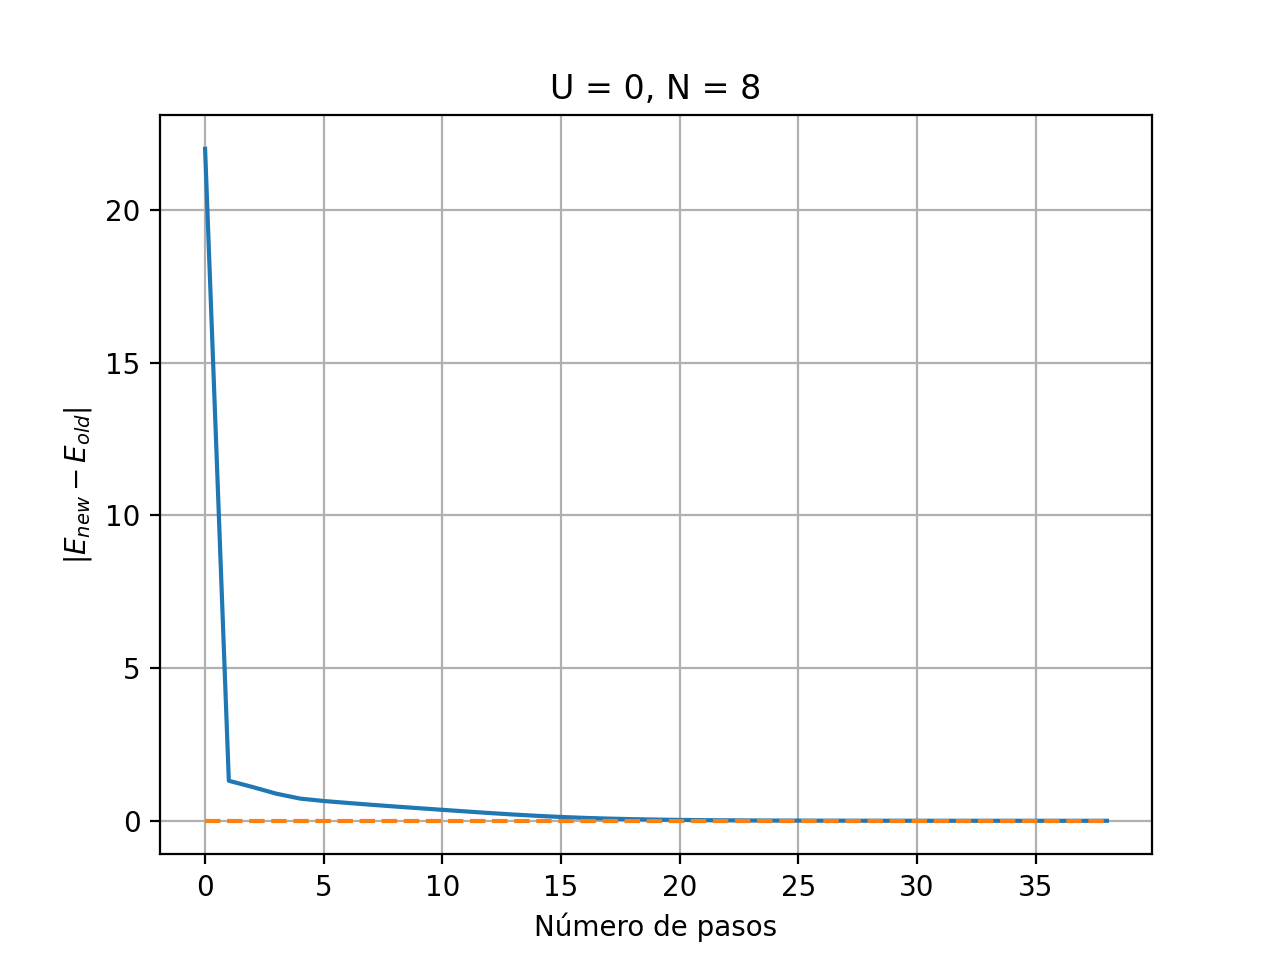
\includegraphics[max width=0.49\linewidth]{convergenceU0N8.png}
  \end{center}
  \caption{Resultados para la convergencia de cadenas de distinto tamaño con un término de interacción $U = 0$.}
  \label{fig:convergenceGood}
\end{figure}

En la primera de estas figuras podemos ver lo que esperábamos, un rápido decaimiento al principio de la distancia entre energías a cada paso, y luego el proceso se va ralentizando paulatinamente. Sin embargo, observemos la figura \ref{fig:convergenceBad}
\begin{figure}
  \begin{center}
    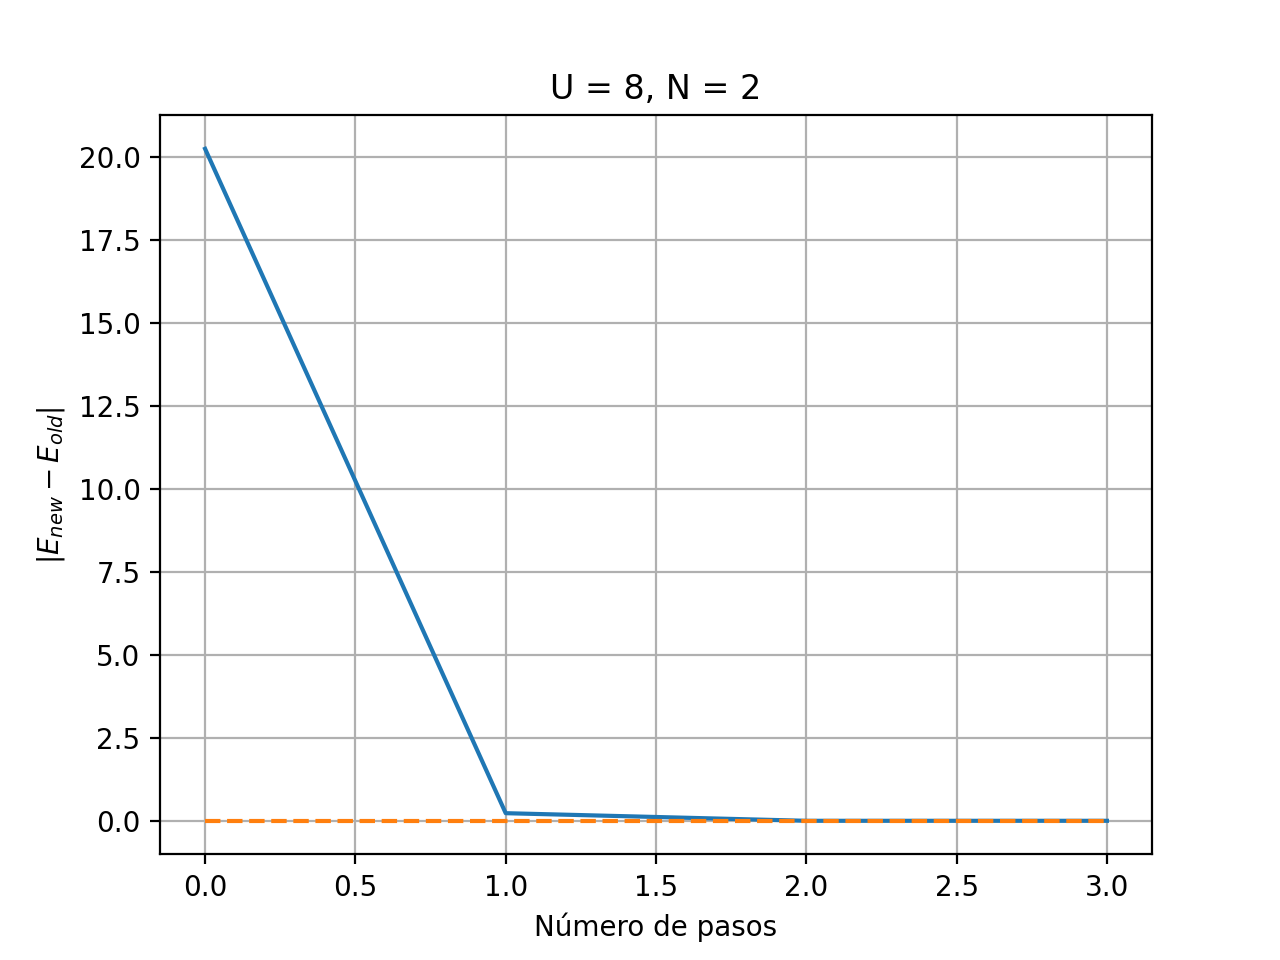
\includegraphics[max width=0.49\linewidth]{convergenceU8N2.png}
    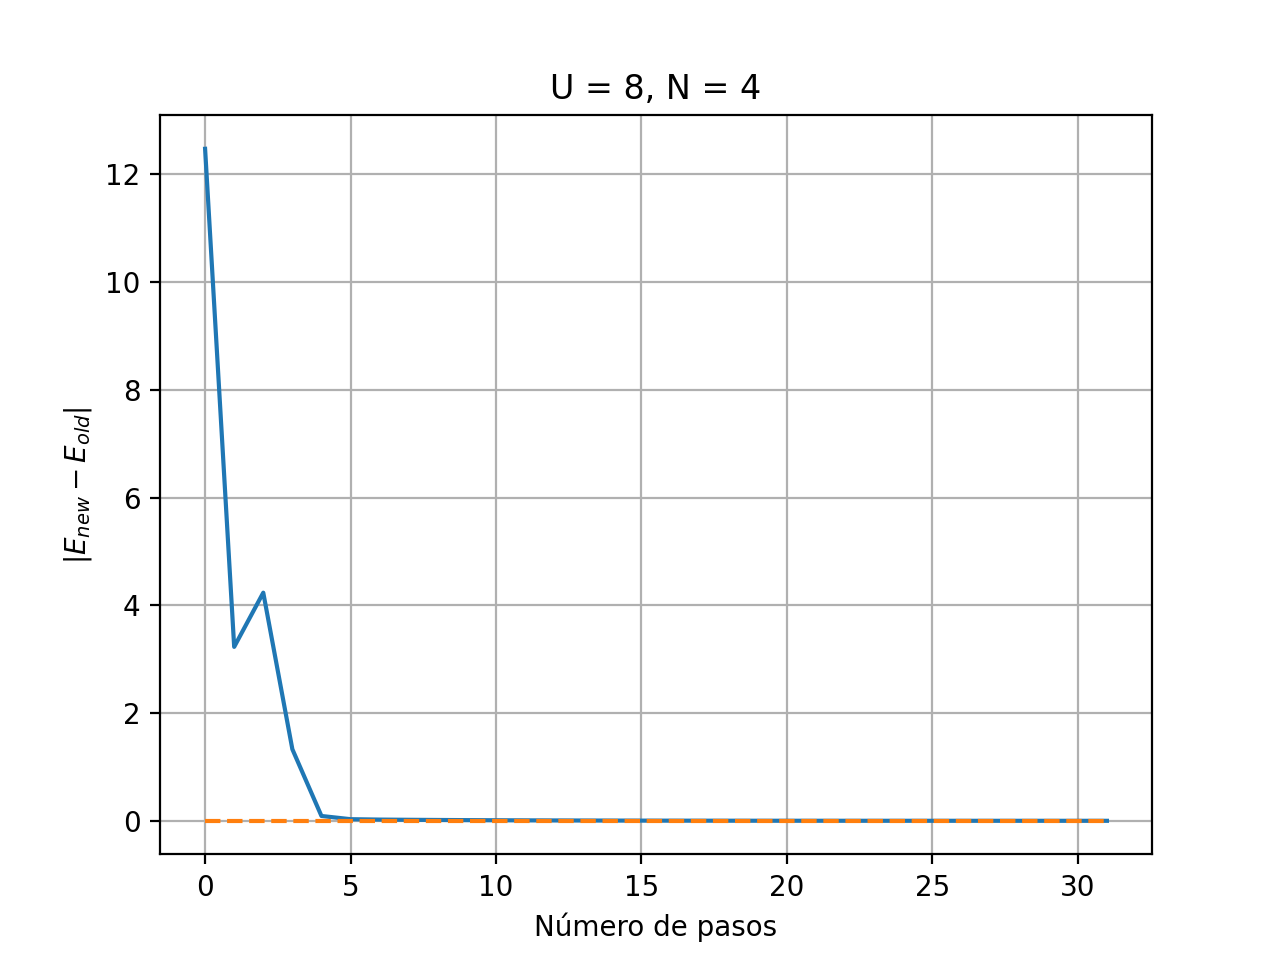
\includegraphics[max width=0.49\linewidth]{convergenceU8N4.png}
    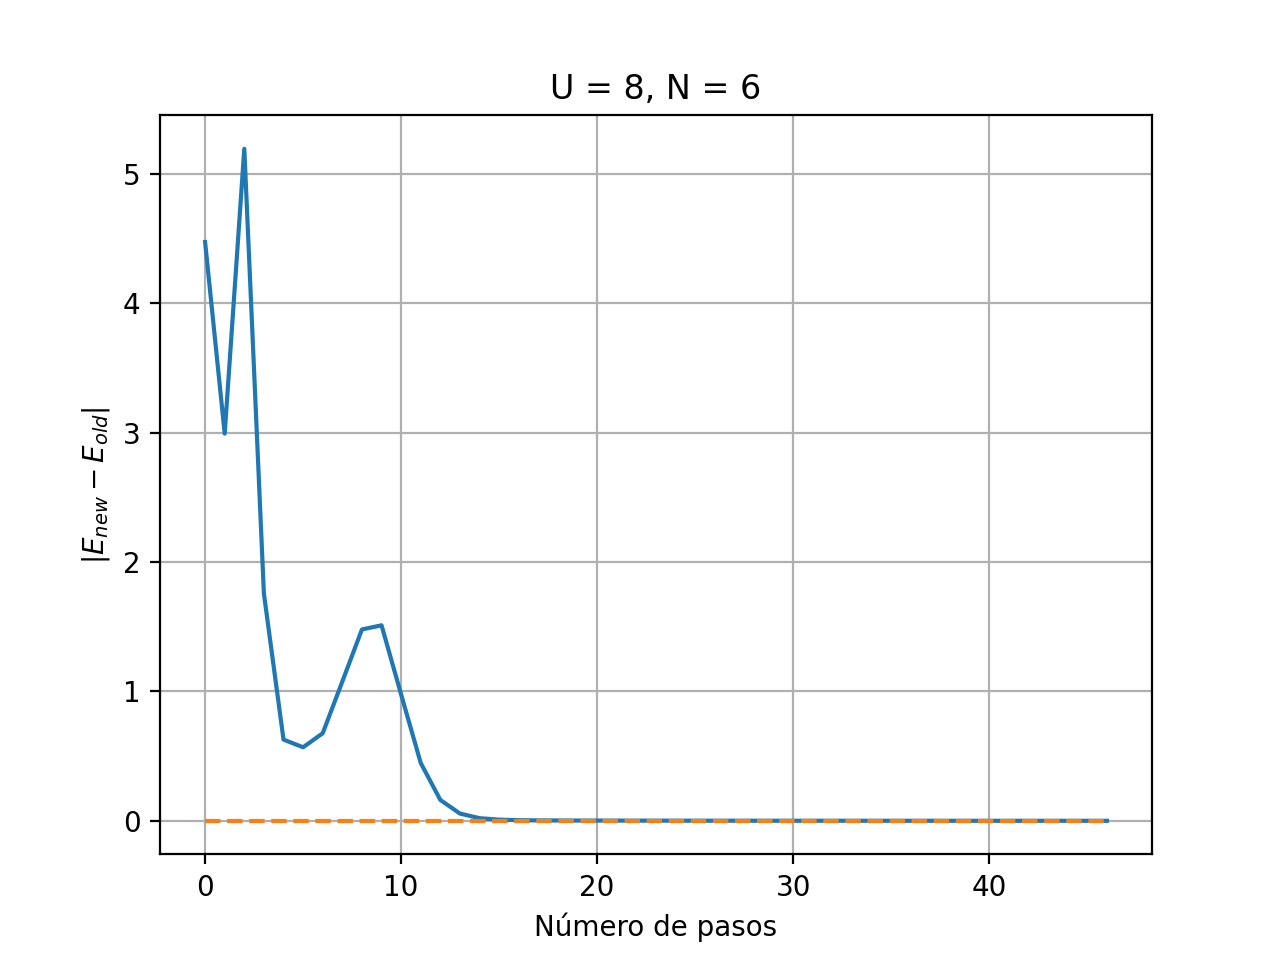
\includegraphics[max width=0.49\linewidth]{convergenceU8N6.png}
    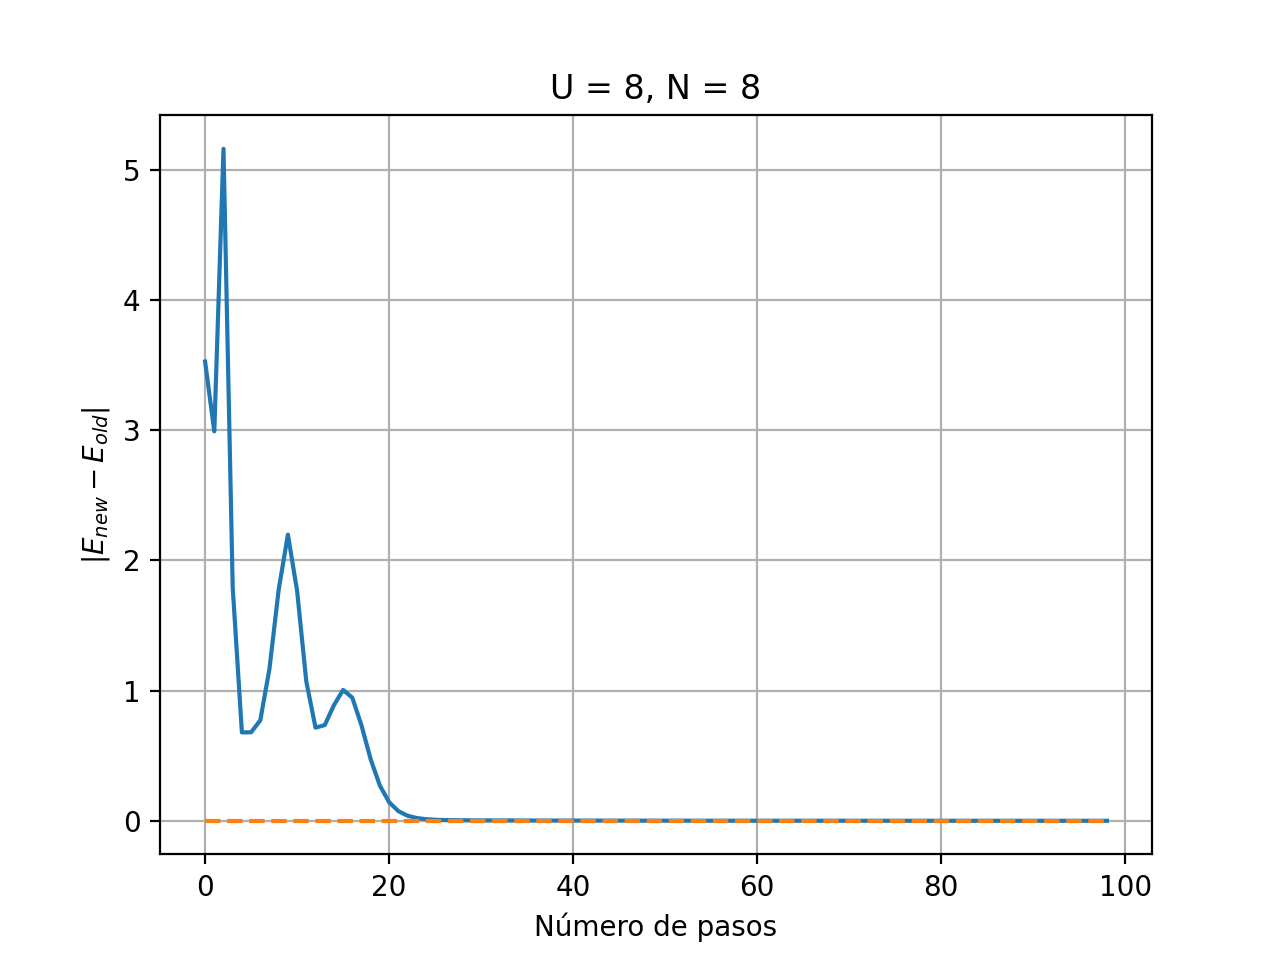
\includegraphics[max width=0.49\linewidth]{convergenceU8N8.png}
  \end{center}
  \caption{Resultados para la convergencia de cadenas de distinto tamaño con un término de interacción $U = 8$.}
  \label{fig:convergenceBad}
\end{figure}

Podemos observar, que al añadir una interacción muy fuerte, la convergencia empieza a ser más lenta y aparecen picos, es decir, al principio le cuesta converger. Una vez hemos avanzado algo más hacia el estado fundamental, observamos que el algoritmo empieza a converger como el caso de la figura \ref{fig:convergenceGood}.

Sin embargo, este comportamiento no se aprecia para el caso $U = 2$, que tiene una forma idéntica a las de la figura \ref{fig:convergenceGood}. Puede deberse a que el comportamiento respecto a la no formación de pares up-down es menos agresivo, lo que aporta algo más de movilidad a la hora de iterar para calcular el estado fundamental.

Finalmente, me gustaría volver a la figura \ref{fig:calcTimes}, puesto que podemos ver que, al ser la gráfica logarítmica, el orden del cálculo debe de ser exponencial, es decir, para una cadena de Hubbard, el algoritmo de Lanczos modificado parece crecer en tiempo de forma exponencial. Diremos entonces que el algoritmo modificado es de orden $\mathcal{O}\left(10^N\right)$, que es notación o-grande, usada en algoritmia para estudiar el crecimiento asintótico en el infinito de una función. Por lo que nuestro tiempo crece en el infinito como $10^N$.
\newpage
\section{Conclusiones}

En conclusión, el modelo de Hubbard modeliza interesantes fenómenos de la materia condensada. En este trabajo hemos podido observar la aparición de superconductividad BCS protegida frente a defectos, así como la transición de metal a aislante. El modelo resulta una importante herramienta, incluso a día de hoy para el estudio de las propiedades de muchos materiales y en algunos modelos DFT.

A lo largo del trabajo hemos entendido la importancia de trabajar en el formalismo de segunda cuantización, puesto que nos ha permitido analizar el modelo de Hubbard de una forma muy sencilla computacionalmente. A su vez, hemos descubierto la potencia de las funciones de Green para calcular propiedades de un sistema y todo el espectro de excitaciones a partir del estado fundamental.

Finalmente, hemos descubierto el algoritmo de Lanczos y programado una clase de Python que nos permite modelizar cualquier vector en el espacio de $|spin\rangle\otimes|orbitales\rangle\otimes|posiciones\rangle$. Sobre esta clase, se ha programado la lógica de los operadores de creación y destrucción de segunda cuantización, así como métodos para sumar vectores y hacer el producto escalar entre ellos.

Hemos creado una potente herramienta para problemas de este tipo en segunda cuantización, que estandariza la programación a una forma mucho más legible. Al crear la nueva clase "Vector", que encapsula todo el comportamiento del tipo de funciones de onda que trabajamos y nos permite aplicar los operadores de creación y destrucción sobre ellos. Por ejemplo, observemos la figura \ref{fig:hubbardCode}, en ella vemos cómo de sencillo resulta programar el hamiltoniano de Hubbard una vez está toda la lógica tras la clase vector y los operadores de creación y destrucción creada.
\begin{figure}[h!]
  \begin{center}
    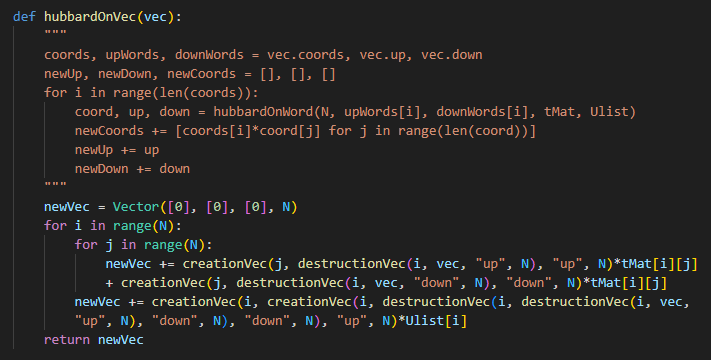
\includegraphics[max width=\linewidth]{HubbardCode.png}
  \end{center}
  \caption{Captura tomada del código para resolver por el método de Lanczos el hamiltoniano de Hubbard, en ella se observa cómo se ha programado el hamiltoniano de Hubbard gracias al uso de las funciones y clases ya programadas.}
  \label{fig:hubbardCode}
\end{figure}

Con sus pros y sus contras, el algoritmo de Lanczos ha sido una potente herramienta que nos ha ayudado a desentrañar el modelo de Hubbard. Desde calcular el estado fundamental a las funciones de Green. El algoritmo de Lanczos es muy potente para tridiagonalizar cualquier hamiltoniano y tiene una rápida convergencia al estado fundamental en su modalidad modificada. Sin embargo, también puede presentar mucho ruido en según que condiciones, pero sigue siendo una herramienta muy potente.

Resumiendo, en el modelo de Hubbard hemos encontrado dos fenómenos muy interesantes que ocurren en los sólidos modelizados por este hamiltoniano:
\begin{itemize}
  \item \textit{Transición metal-aislante.} Al hacer una interacción $U>0$, el sistema tiende a no formar pares electrón-electrón. Además, aparece un desdoblamiento de las bandas, lo que genera una pérdida de la conductividad frente al modelo tight-binding, haciendo una transición metal-aislante y convirtiendo el material en aislante debido a la aparición de la interacción.
  \item \textit{Superconductividad.} Al cambiar el signo de la interacción y hacerla negativa, el estado fundamental presenta pares up-down, que además, están protegidos frente a defectos en el material, dotándole de propiedades superconductoras.
\end{itemize}

En resumen, el modelo de Hubbard es un modelo sencillo que nos permite modelizar ciertos sólidos que presentan interacción entre electrones, y estas interacciones dotan al material de propiedades interesantes.

Las aplicaciones de este modelo en el mundo real son muchas. El modelo es utilizado para cálculos básicos en simulaciones DFT para predecir la transición de fase, además, nos da una forma simple de estudiar muchos fenómenos interesantes. A día de hoy, el modelo de Hubbard es estudiado todavía ampliamente por los fenómenos que reproduce.

Este modelo nos ha dotado de herramientas para entender la superconductividad BCS, que además, aparece protegida frente a defectos en la red, gracias a la fuerza con la que se forman los pares de electrones up-down.

Finalmente, hemos utilizado las funciones de Green como herramienta para entender muchas propiedades del sistema y encontrar la densidad de estados del sistema, aplicando diversos conocimientos nuevos que no se estudian en la carrera: segunda cuantización, funciones de Green, etc.

A lo largo del trabajo se han aplicado también conceptos de asignaturas como física del estado sólido, física cuántica avanzada o mecánica cuántica II. Siendo un trabajo multidisciplinar en este aspecto, en el que se aplican diversos conceptos, nuevos y ya vistos en la carrera.

Como conclusión, el modelo de Hubbard ha resultado muy interesante, y a lo largo de este trabajo he podido leer muchas fuentes, artículos, libros, revistas, etc. y he podido aprender mucho sobre funciones de Green y cuántica de muchas partículas, un área en el que deseo adentrarme más a futuro. Ha sido un placer hacer este trabajo y lo he disfrutado mucho. A futuro, el modelo de Hubbard aún tiene camino como forma de introducirse en este mundo de la teoría de materiales, y seguirá siendo un buen caso de estudio para los estudiantes que quieran introducirse a este área, así como un modelo ampliamente utilizado hoy en día en muchas partes de la física de la materia condensada.

Finalmente, agradecer a Guillermo, ya que no lo hice en la sección de agradecimientos, pero creo que merecía una mención aparte. Por ser un gran tutor, proponer un tema muy interesante que ya decidimos antes de empezar cuarto curso y ayudarme en todos los correos y reuniones en su despacho. También, gracias por sentarse conmigo a revisar los últimos borradores de este trabajo, que al final sufrieron bastantes cambios gracias a estas reuniones. No podría estar más contento de haberlo elegido como tutor.
\newpage
\addcontentsline{toc}{section}{Referencias}

\printbibliography

\end{document}